\usepackage{tabularx}

\newcommand*{\zee}{$Z \to e^{+}e^{-}$\xspace}
\newcommand*{\et}{$E_{\text{T}}$\xspace}
\newcommand*{\zmass}{$\text{Z}_{\text{mass}}$\xspace}
\newcommand*{\ziso}{$\text{Z}_{\text{iso}}$\xspace}
\newcommand*{\tp}{T$\&$P\xspace}
\newcommand*{\et}{$E_{\text{T}}$\xspace}
\newcommand*{\eta}{$\eta$\xspace}

\setcounter{secnumdepth}{3}

Electrons play a crucial role in the ATLAS physics programme, appearing in key final states from precision electroweak measurements to Higgs boson studies and BSM searches. For this reason, accurate reconstruction, identification, calibration and isolation are critical to achieving the ATLAS experiment’s scientific goals in most analyses.  

Although the basic workflow for constructing electron candidates mirrors the one already explained for other physics objects in Chapter~\ref{chap:object_rec}, the performance demands on electrons are particularly stringent, from the precision with which tracks and energy clusters are reconstructed to achieving the best possible agreement between recorded data and the Monte Carlo simulations.  

In the following chapter we delve into how electrons are treated, defined and calibrated in ATLAS, especially because part of the work in this thesis has focused on the study and refinement of a DNN for electron identification and classification against other objects that can mimic their signature.  The architecture of this ML algorithm is going to be shown, as well as the electron features that are used as inputs, its performance, and how its output is handled. 

This DNN is introduced as an improved method intended to replace the likelihood-based approach employed since the beginning of Run-2, which is also discussed here.  Finally, we compare efficiency measurements for prompt electrons obtained with both techniques and derive scale factors to correct any mismatches between performance in data and in MC simulation.  These efficiencies are measured in data using tag-and-probe techniques on a pure and unbiased sample of electrons, typically drawn from well-known physics processes rich in prompt electrons such as the decay $Z\to e^+e^-$, an example of which is illustrated in the event display in Figure~\ref{fig:zee}.

\begin{figure}[htbp]
    \centering
    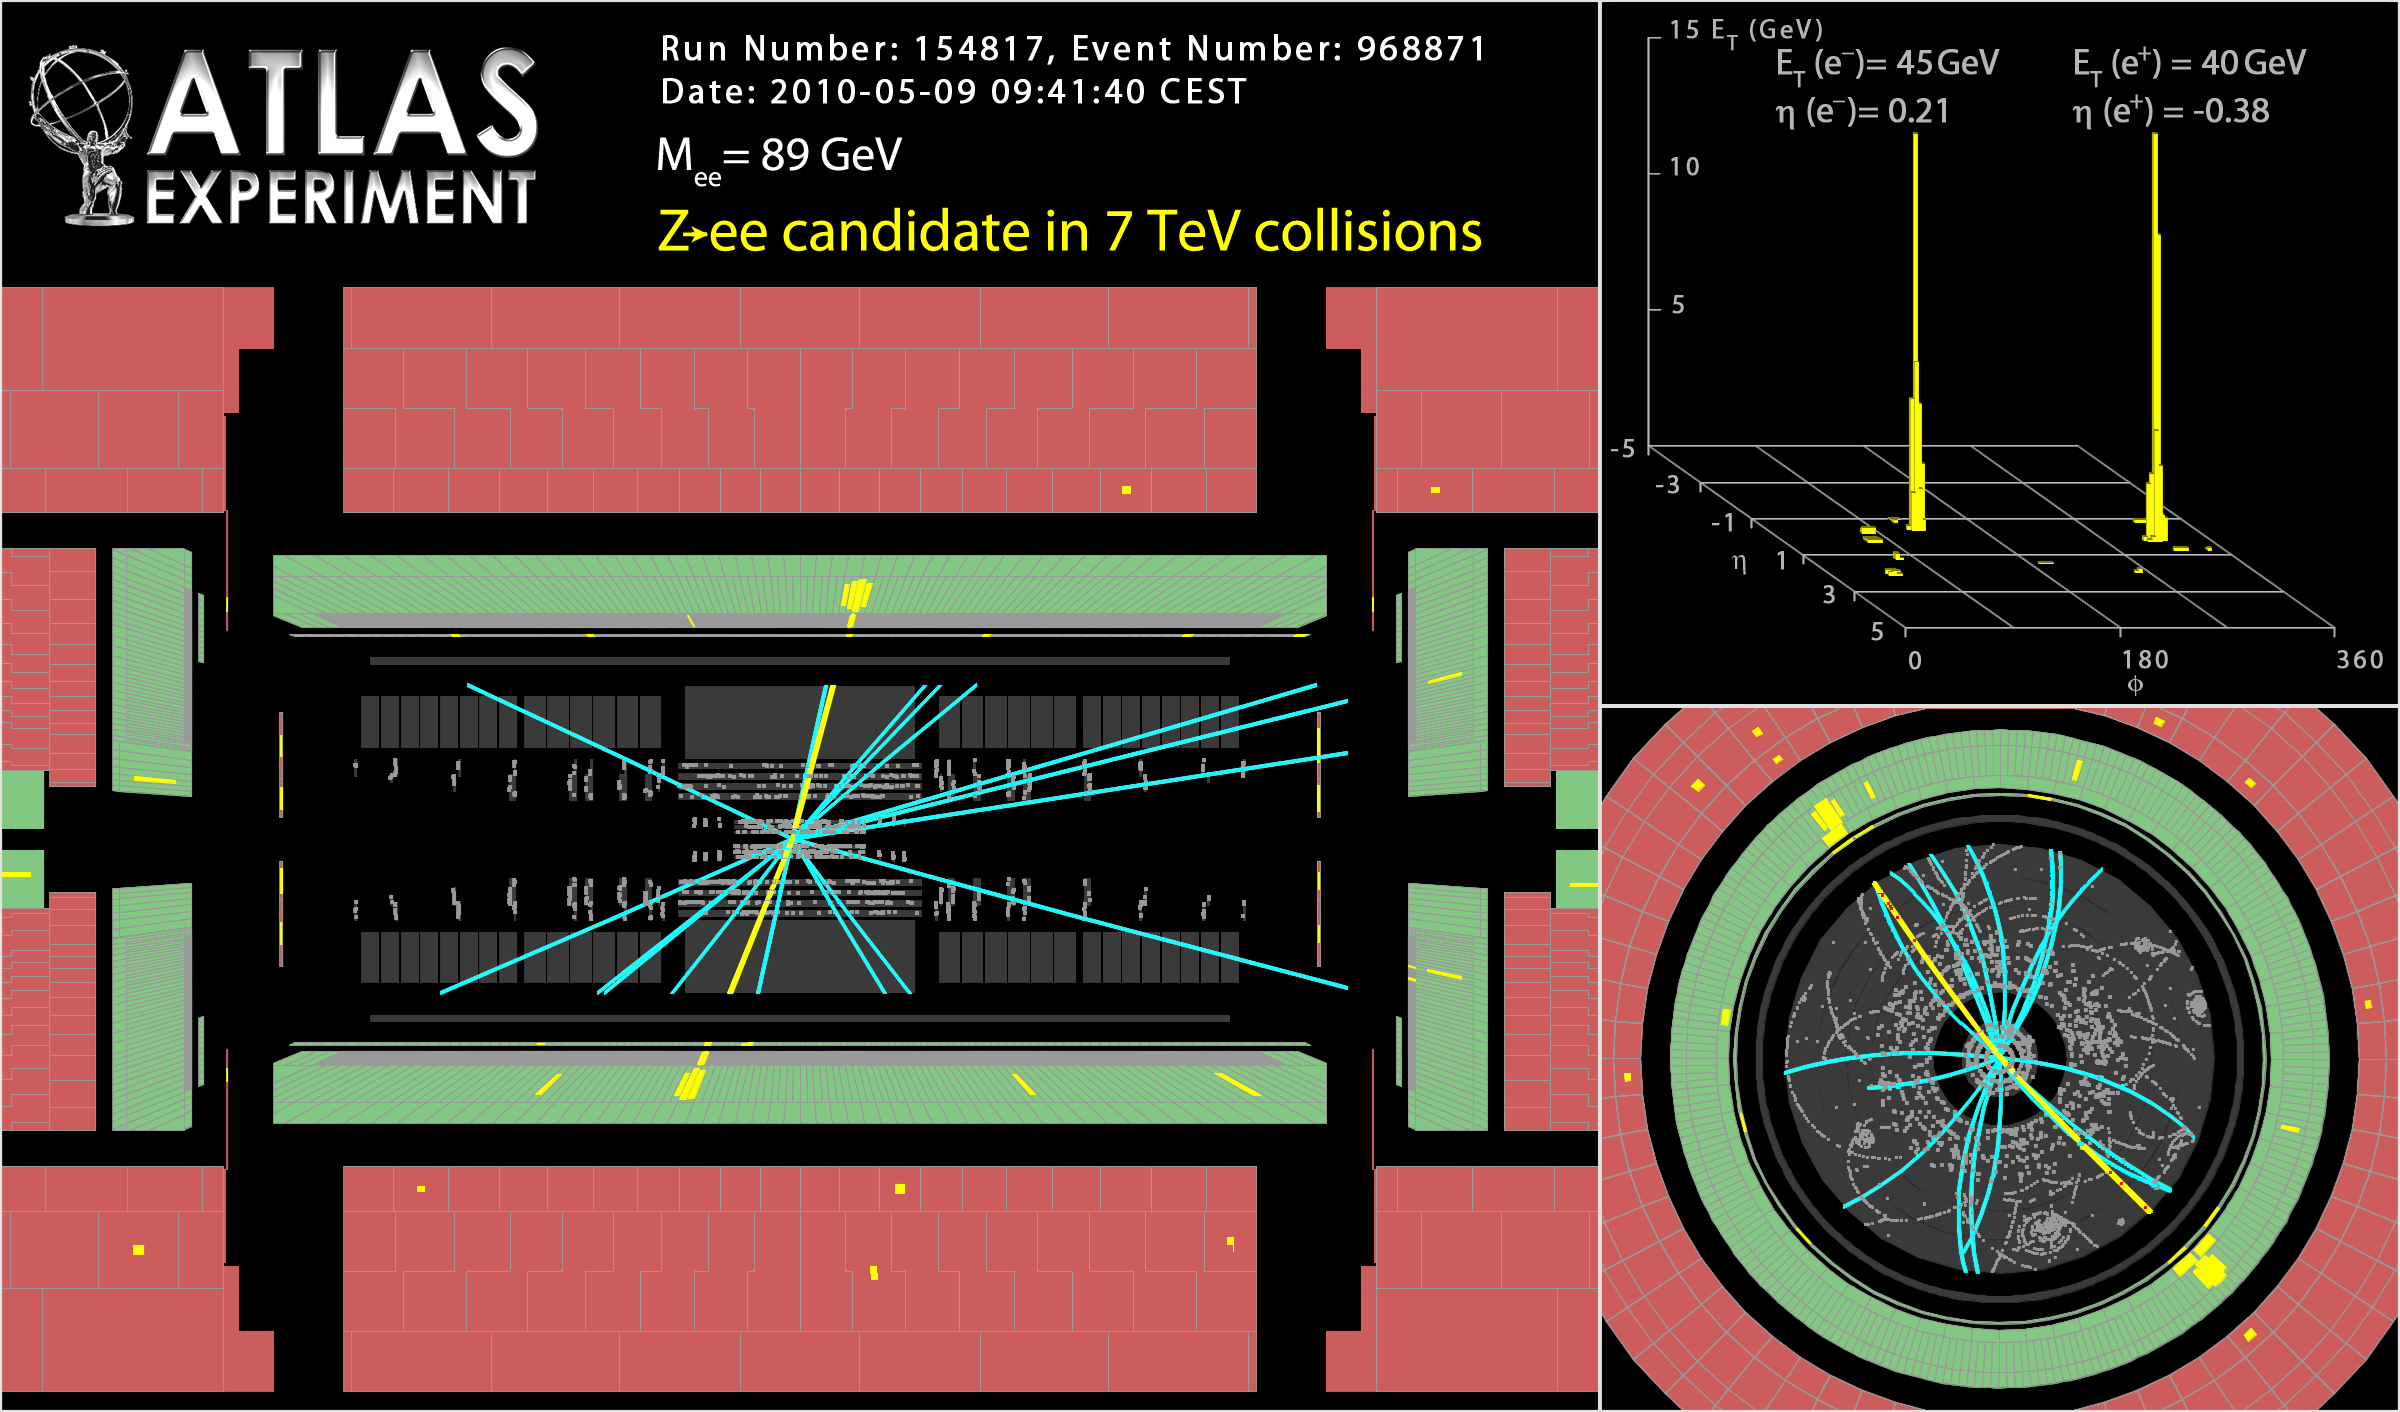
\includegraphics[width=0.7\textwidth]{images/Zee.png}
    \caption{ATLAS reconstructed event display of a candidate for a $Z\to e^+e^-$ decay, collected on 9 May 2010. The two electrons are well isolated and represented with yellow lines. Further event properties: $p_{T}(e^{+})$ = 40~GeV, $p_{T}(e^{-})$ = 45~GeV, $\eta(e^{+}) = -0.38$, $\eta(e^{-}) = 0.21$, $m_{e^{+}e^{-}}=89$~GeV~\cite{atlas:eventdisplay}. }
    \label{fig:zee}
\end{figure}

The rest of this chapter therefore covers the reconstruction inputs and calibration steps that define ATLAS electrons, the architecture and training of the new DNN ID, the tag-and-probe procedures used to extract data-driven efficiencies, and, finally, a direct comparison of DNN ID performance against the Run-2 likelihood benchmark. Together, these studies quantify the improvements in signal efficiency and background rejection achieved by the neural-network approach and lay the groundwork for its deployment in Run-3 analyses.  

%%%%%%%%%%%%%%%%%%%%%%%%%%%%%%%%%%%%%%%%%%%%%%%%%%%%%%%%%%%%%%%%%%%%%%%%%%%%%%%%%%%%%%%%%%%%%%%%%%%%%%%%%%%%%%%%%%%%%%%%%%%%%%%%%%%%%%%%%%%%%%%%%%%%%%%%%%%%%%%%%%%%%%%%%%%%%%%%%%%%%%%%%%%%%%%%%%%%%%%%%%%%
\section{Electron Reconstruction}

In the ATLAS detector, an electron can be reconstructed when its electromagnetic energy deposits in the calorimeter system can be matched to a charged-particle track in the Inner Detector. Figure~\ref{electron_journey} illustrates the typical journey of an electron traversing the various layers of ATLAS, from the interaction point outwards.

\begin{figure}[htbp]
  \centering
  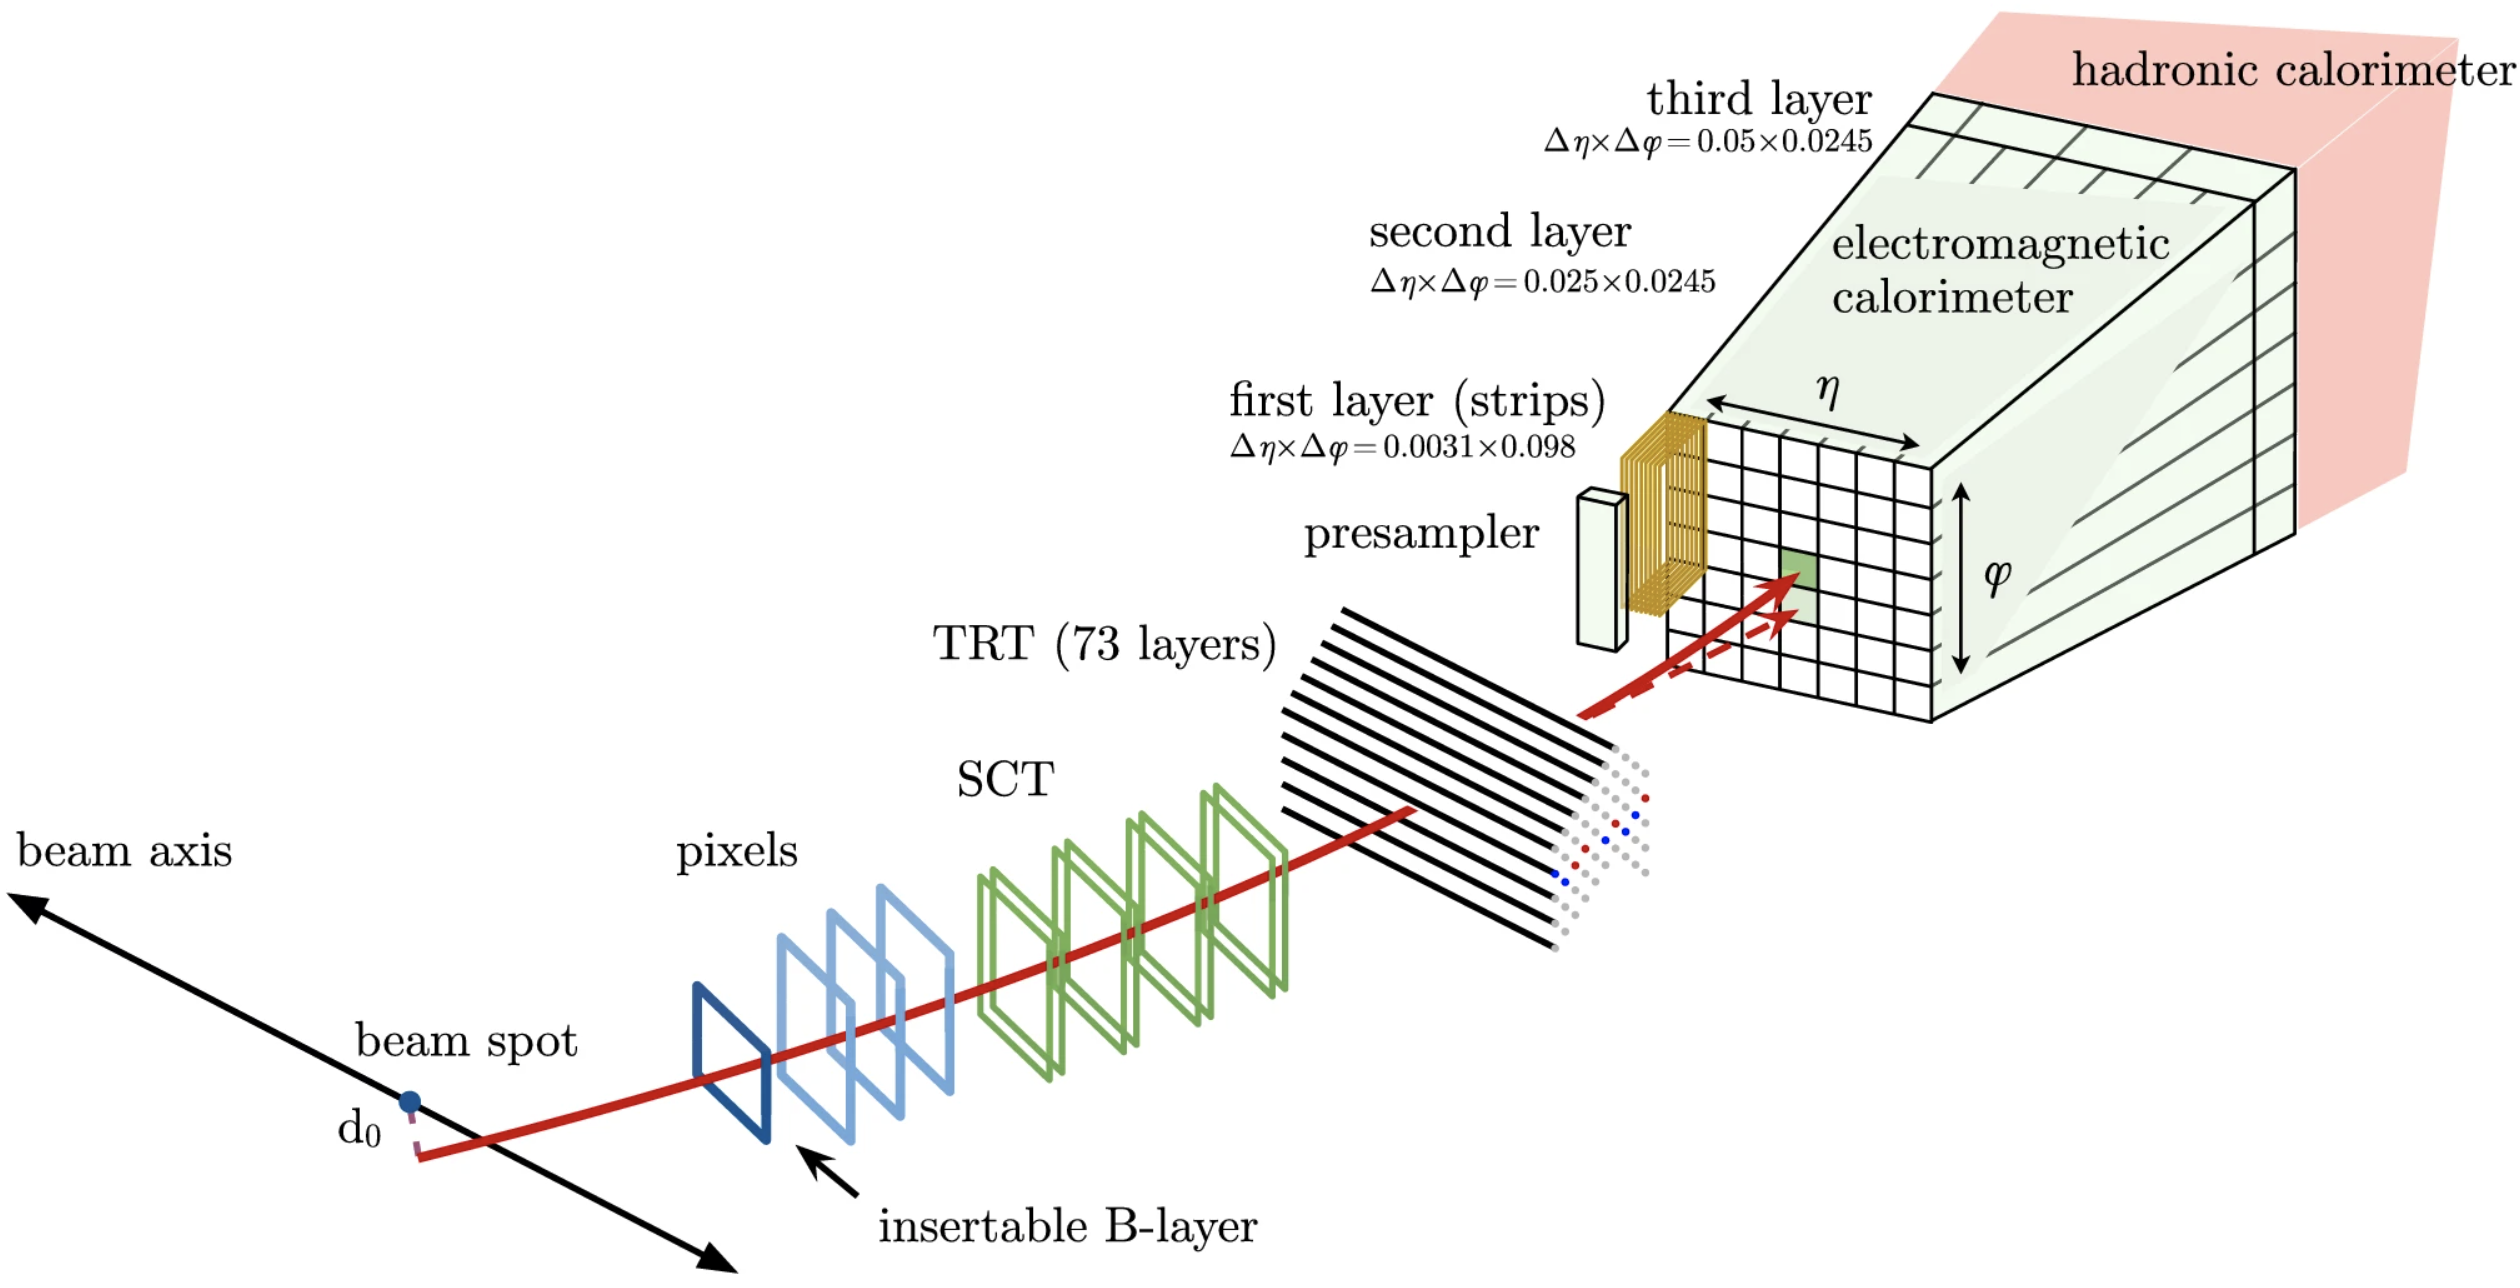
\includegraphics[width=0.8\textwidth]{images/electron_journey.png}
  \caption{Illustration of the typical journey of an electron passing through ATLAS. In red it is represented its expected path, first going through the tracking system. Afterwards it leaves mostly all its energy in the electromagnetic calorimeter. It can be also found the possible path (dashed red) of photon radiated by bremsstrahlung when the electron interacts with the material~\cite{Aaboud:2657964}.}
  \label{electron_journey}
\end{figure}
One can say that there are three stages in reconstructing an electron: although it first traverses the various pixel and silicon layers of the ID plus the network of TRT straw tubes before depositing most of its energy in the electromagnetic calorimeter through bremsstrahlung radiation, the reconstruction of an electron candidate actually begins with the identification of clusters of calorimeter cells containing this electromagnetic energy. After the clustering, 
the tracks in the ID are reconstructed and classified, as detailed in Section~\ref{sec:tracks}. The final step is to efficiently match these tracks to the electromagnetic clusters to form electron candidates, being able to distinguish them from other objects such as charged pions.

\subsection{Cluster Building}

The dynamic algorithm for defining variable-size clusters of cells from the calorimeters was implemented in Run-2~\cite{dyn_clust}, yielding performance that far surpasses the fixed-size algorithm used in the previous data-taking period~\cite{fix_clust}.

These dynamically sized clusters, known as topological clusters (topoclusters), grow around a seed cell defined according to an algorithm detailed in Ref.~\cite{fix_clust}. A seed must satisfy a cell significance of $\epsilon_{\text{cell}}^{\text{EM}} \geq 4$
and cannot be located in the presampler or the first layer of the electromagnetic calorimeter. This significance is defined as
\begin{equation}
  \epsilon_{\text{cell}}^{\text{EM}} = \frac{E_{\text{cell}}^{\text{EM}}}{\sigma^{\text{EM}}_{\text{noise,cell}}},
\end{equation}
being \(E_{\text{cell}}^{\text{EM}}\) the energy of the given cell and \(\sigma^{\text{EM}}_{\text{noise,cell}}\) its expected noise.

The significance of all cells neighboring the seed cell is then evaluated, and any cell with $\epsilon_{\text{cell}}^{\text{EM}} \geq 2$ is added to the cluster. This procedure iterates, treating each newly added cell as the seed for the next step, forming a growing protocluster. Protoclusters sharing a cell are merged, and once no further high-significance cells can be included, a final growth step adds all adjacent cells regardless of their significance. If the resulting topocluster contains more than one local maximum, it is split into separate clusters, each centered on one maximum cell. A local maximum is defined as a cell with \(E_{\text{cell}}^{\text{EM}}>500\)~MeV that has at least four neighbors of lower energy.

For electron reconstruction, only the energy deposited in the electromagnetic calorimeter is used, excluding any energy in the transition region \(1.37<|\eta|<1.52\). 
Contributions from the presampler and the first EM layer are also added when computing the cluster’s electromagnetic energy. The electromagnetic fraction, \(f_{\text{EM}}\), is defined as the ratio of this EM energy to the cluster’s total energy. To suppress clusters from pile-up or hadronic activity, only those with \(f_{\text{EM}}>0.5\), \(E_{\text{EM}}>400\)\,MeV, and at least half of their energy in the ECAL are retained as electron candidates.  

\subsection{Track-to-Cluster Matching}

For electron candidates, the standard tracking algorithm explained in Section~\ref{sec:tracks} is extended to account for electrons losing energy via bremsstrahlung as they traverse the ID detector materials. 

Initially, tracks are fitted under a pion hypothesis assuming an ideal helical trajectory~\cite{tracks}. If this fit fails for a given track seed within the region of interest defined by the EM topocluster (i.e., small pseudorapidity separation between track and cluster), the fit is retried with a modified pattern-recognition algorithm based on the Kalman filter formalism~\cite{FRUHWIRTH1987444}, which allows for energy losses at each material intersection due to photon radiation and thus deviations from a perfect helix.

This formalism, called Gaussian Sum Filter (GSF), represents the track state as a weighted sum of Gaussian components, each propagated in parallel via a Kalman filter, modelling the sudden curvature changes induced by discrete photon emissions. After GSF refitting, the tracks are extrapolated to the ECAL and matched to EM topoclusters using asymmetric $\phi$ windows (wider on the side corresponding to expected energy loss) and tight $\eta$ proximity. When multiple tracks match a single cluster, candidates are ranked first by fit quality and then by distance to the cluster barycentre in the second EM layer; the highest-ranked track is chosen to define the electron kinematics.


\subsection{Superclusters and calibration}

In order to capture the full energy deposited by these bremsstrahlung photons from the electron candidate, adjacent EM topoclusters are merged into superclusters, which gather all significant energy deposits along the electron’s radiative path, as represented in Figure~\ref{fig:superclust}.  
\begin{figure}[htbp]
  \centering
  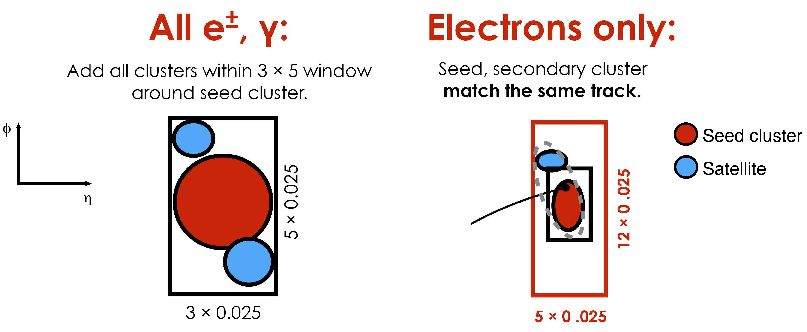
\includegraphics[width=0.8\textwidth]{images/superclusters.png}
  \caption{Schematic overview of the formation of superclusters during electron reconstruction~\cite{Aad:2684552}.}
  \label{fig:superclust}
\end{figure}
Reconstruction of an electron supercluster begins by ordering all electromagnetic topoclusters by their transverse energy and selecting the highest-$E_{\text{T}}$ cluster as the seed. This seed must not already be assigned to another supercluster, and the reconstructed track matched to it must carry at least four hits in either the Pixel detector or the SCT~\cite{Aad:2684552}. Once a valid seed is identified, additional “satellite” topoclusters are incorporated within a sliding window of \(3\times5\) or \(5\times12\) calorimeter cells (corresponding to \(\Delta\eta\times\Delta\phi = 0.075\times0.125\) and \(0.125\times0.300\), respectively) centered on the seed’s energy-weighted barycenter. The smaller window captures nearby secondary electromagnetic showers, while the larger one recovers energy radiated via bremsstrahlung. Finally, the assembled supercluster is matched to its track using the same \(\eta\)-\(\phi\) proximity criteria described before, yielding the fully reconstructed electron object used in subsequent physics analyses.  

However, this reconstruction procedure is based on the raw energy measurements of both electrons and photons, derived from the sum of cell energies. To achieve the highest possible precision, these energy measurements must be calibrated and are therefore firstly optimized via a BDT regression trained on Monte Carlo simulation, which combines the energy deposits across the three longitudinal calorimeter layers. Subsequently, the response of each individual layer is calibrated separately to correct for its \et-dependent behavior, and the same corrections are applied identically to both data and simulation samples.

After layer-by-layer corrections, residual discrepancies between data and simulation, arising from effects such as azimuthal non-uniformities in the calorimeter's granularity, are removed by applying additional region-dependent corrections to the data. Finally, the absolute energy scale and resolution are tuned using large samples of \(Z\to e^+e^-\) decays, ensuring that the reconstructed \(Z\) peak in data aligns with the simulation. Any remaining resolution differences are corrected by smearing the simulated energies, and the overall procedure is validated and its uncertainties quantified using \(J/\psi\to e^+e^-\) events.  

%%%%%%%%%%%%%%%%%%%%%%%%%%%%%%%%%%%%%%%%%%%%%%%%%%%%%%%%%%%%%%%%%%%%%%%%%%%%%%%%%%%%%%%%%%%%%%%%%%%%%%%%%%%%%%%%%%%%%%%%%%%%%%%%%%%%%%%%%%%%%%%%%%%%%%%%%%%%%%%%%%%%%%%%%%%%%%%%%%%%%%%%%%%%%%%%%%%%%%%%%%%%
\section{Electron Identification}

As already mentioned, there are other types of physical objects that can mimic the characteristic signature left by electrons in the ATLAS detector, and can therefore end up being reconstructed as electron candidates. 

In the physics analyses carried out within the collaboration, the background coming from these objects needs to be reduced as much as possible. Moreover, not all real electrons are to be considered as signal in many cases. Only prompt isolated electrons originating from the decay of heavy bosons such as the W, Z, and Higgs bosons are of interest, while those coming from the decay of charged quarks or photon conversions are generally also considered as background.

Therefore, in order to efficiently classify the electron candidates of interest, a set of selections must be applied to the candidates after the reconstruction step, which is what is known as identification. To identify the types of electrons, discriminants are typically defined based on observables or features of the physical objects that allow for a discrimination between prompt and background electrons, for instance, since it is a generic procedure adopted for other types of physical objects as well, both in ATLAS and in other experiments such as CMS.

These discriminants can be defined in various ways, and the following describes the Likelihood-based approach, used since the beginning of the Run-2 period, and the novel identification algorithm based on a DNN.

Finally, the identification process is completed by using the output of that discriminant, on which certain thresholds are defined targeting specific values of signal identification efficiency and background rejection. Since the behaviour of electrons generally varies as a function of their energy and of the detector region under consideration, these thresholds are typically defined in bins of the electron’s \et and $\eta$, and are encapsulated in what are known as identification Working Points (WPs). These WPs generally also include other requirements on additional variables, as will be seen later, and finally different working points obtained from the same discriminant or approach are grouped into identification menus, which are ultimately what is provided from the Combined Performance (CP) groups to the physics analysis groups.

\subsection{Likelihood-based identification}

So far, electron identification in ATLAS has been based on a Likelihood (LH) approach~\cite{Aad:2684552,Aaboud:2657964}, which relies on a wide range of information from different detector subsystems. This algorithm uses high-level input variables defined from the properties of electrons and the information they leave as they pass through the detector. These variables will be detailed later, since they are largely shared with the DNN, and further information can be found in Ref.~\cite{Aaboud:2657964}.

A central aspect in the construction of the LH discriminant is the definition of one-dimensional Probability Density Functions (PDFs) for each input variable. It is done separately for signal and background electrons, based either on real data or on the simulations previously described.
The discriminant is then constructed from these PDFs, which reveals one of the limitations of this method: the correlations between variables are lost when creating these density functions, which are obtained by applying a Kernel Density Estimator (KDE) to the histograms of each variable separately, using the TMVA toolkit~\cite{tmvatoolkit}. 

Therefore, the likelihood of an electron candidate being signal ($L_{\text{S}}$) or background ($L_{\text{B}}$) is given by:

\begin{equation}
  L_{\text{S(B)}} (\textbf{x}) = \prod_{i} P_{\text{S(B)},i}(x_{i}),
\end{equation}
where $P_{\text{S(B)},i}(x_{i})$ are the signal (background) PDFs, and $x_{i}$ is simply the value of the $i$-th input variable, so the likelihood is just the product of all PDFs.
Then, the likelihood discriminant, $d_{L}$, is simply obtained as:
\begin{equation}
  d_{L} = \frac{L_{\text{S}}}{L_{\text{S}} + L_{\text{B}}},
\end{equation}
which achieves the goal of clearly separating the signal and background distributions, as can be seen in the example of Figure~\ref{fig:lhdis}.
\begin{figure}[htbp]
  \centering
  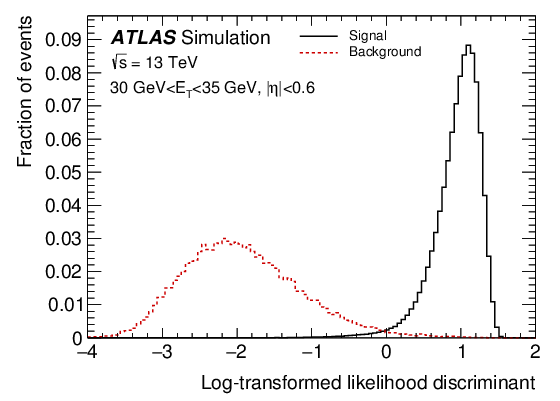
\includegraphics[width=0.6\textwidth]{images/lhdis.png}
  \caption{Likelihood discriminant distributions obtained in a particular \et and $\eta$ bin, for signal and background computed for simulated electrons corresponding to R.21 Run-2 period~\cite{Aaboud:2657964}. An additional monotonic transformation is applied to the discriminants which does not change its classification power.}
  \label{fig:lhdis}
\end{figure}

As previously mentioned, the PDFs of the variables are parametrised in different bins of \et and $\eta$, and the same applies when building the discriminant and defining the thresholds that form the Working Points (WPs).

The requirements additional to these cuts on the discriminant, and applied to determine whether an electron candidate passes a given WP, include a certain number of hits in different parts of the tracking detectors and also requirements on the ambiguity type. This ambiguity type is a sort of flag assigned to the candidate during reconstruction, providing information on whether the topocluster associated with the electron was also reconstructed as a photon.
Each WP encapsulates different requirements, and in this thesis we use $LHLoose$, $LHMedium$, and $LHTight$, ordered from highest to lowest in signal identification efficiency, and the reverse in terms of background rejection. They are subsets of each other, meaning that if an electron passes the $LHTight$ WP, it also passes the other two.

Regarding the LH menu used in subsequent calculations, the PDFs were obtained from data for the signal in order to ensure the best possible performance when applied to real data, and also for the background PDFs, as these result in distributions that are even less signal-like than those derived from Monte Carlo simulations. This is precisely what is desired for the method to work efficiently.

The selection used to obtain the purest possible sample of candidates for both types is fully detailed in Ref.~\cite{lucas_thesis}. In summary, in order to construct the Probability Density Functions (PDFs) a tag-and-probe method is applied. Signal electrons are selected from $Z \rightarrow e^{+}e^{-}$ or $J/\psi \rightarrow e^{+}e^{-}$ decays. Events with $E_{\text{T}} > 15$~GeV are taken from $Z$ decays, while lower-$E_{\text{T}}$ electrons ($E_{\text{T}} \leq 15$~GeV) come from $J/\psi$ decays. A tightly identified and isolated “tag” electron is required, and a “probe” electron is selected if the invariant mass of the pair matches the $Z$ or $J/\psi$ boson mass. No further ID or isolation requirements are applied to the probe, ensuring unbiased signal distributions.

Background PDFs are obtained from multi-jet events. Due to their large cross-section, loose selection of reconstructed electrons yields mostly background. To improve purity, $Z \rightarrow e^{+}e^{-}$ and $W \rightarrow e\nu$ decays are vetoed. The $Z$ veto removes events with a second electron forming a mass near the $Z$ boson. The $W$ veto applies a cut on it transverse mass, which also removes electrons from top-quark decays.


\subsection{Deep neural network for electron identification}
\label{subsec:dnn_id}
%Small introduction about the DNN: why is a good alternative? Reference the DNN paper, and the Statistical methods section for more info about DNNs. Talk a bit about what is going to be shown heres

Electron identification in ATLAS has historically been performed without the use of machine learning. During the Run-1 period, a cut-based selection was used, applying rectangular cuts directly optimised on characteristic observables of the electron candidates. Later, during Run-2, the strategy evolved into the LH approach, described in the previous section.

While the LH method has proven effective selecting signal electrons with high efficiency and background rejection, recent advances in ML have introduced new possibilities for improving classification performance and signal-to-background discrimination in high energy physics. In particular, deep neural networks (DNNs) have demonstrated a strong ability to model complex correlations among input variables, overcoming one of the main limitations of the LH model.

This section presents an alternative algorithm based on a DNN, developed as an improved replacement for the LH discriminant using a similar set of high-level input variables.

A detailed technical description of the implemented algorithm can be found in Ref.~\cite{dnn_paper}, initially developed and validated for Run-2 Release 21. More general information on the statistical principles and methodology of neural networks is provided in Section~\ref{sec:ml_methods}.

Here, the focus is placed on the specific application to electron identification, training and optimising the DNN using simulated samples to distinguish prompt isolated electrons from various background sources. The following describes the selection of samples and the definition of training classes, the choice and preprocessing of input variables, the training procedure and performance, and finally, the definition of the working points derived from the DNN output.

\subsubsection{Samples and electrons selection}
%Mention that samples used here were already presented in Section~\ref{subsec:electron_mc}. Define which selection is applied to electrons used in the training, and also introduce
%how the different classes are defined. Talk about how input n-tuples are produced a bit.
The first step to prepare the DNN for electron identification is to define the training, validation, and test datasets that will feed the algorithm. As previously mentioned, simulated electron candidates are used for this purpose, extracted from different processes generated as described in Section~\ref{subsec:electron_mc}, corresponding to the Run-2 R.22 period.

Signal electrons are selected from $Z \rightarrow e^{+}e^{-}$ decays, complemented with $J/\psi \rightarrow e^{+}e^{-}$ resonances to increase statistics in the low-\et region. As sources of the main background classes that mimic electron-like signatures, we use the $JF17$ sample, complemented with a sample of simulated \ttbar events, from which only events containing at least one lepton in the final state are considered.

These samples are processed through the \textsc{TagAndProbe} analysis software, a \textsc{GitLab}~\cite{tagandprobe} project maintained by the Combined Performance $e/\gamma$ group, focused on the treatment and performance measurements of electrons and photons in ATLAS. This framework provides a convenient format for storing the electron candidates of each type, allowing for the application of certain quality prerequisites.

In our case, this preselection is minimal and consists of requiring all reconstructed electrons to have a transverse energy of at least $4.5$~GeV, a minimum of one hit in the pixel subdetector, and at least seven hits in the silicon detector systems. Additionally, only electrons within the region $|\eta| < 2.47$ are considered. The electron candidates are corrected for energy scale and resolution using the \textsc{TagAndProbe} framework, and further selection criteria are applied to reject candidates associated with problematic detector regions or poorly reconstructed calorimeter clusters.

Finally, it is important to note that, from $Z$-boson decays, only electron candidates with \et$>15$~GeV are used, since lower-energy regions suffer from an increased population of background electrons. For \et below this threshold, electrons from $J/\psi$ decays are used instead. Further requirements on the origin of the electrons are applied to ensure that different types of candidates are selected from each sample, resulting in six distinct classes, which will be defined in the following.

\subsubsection{Classes}

One of the most important steps when training a supervised classifier like a DNN is the definition of the target classes. In our case, this translates into deciding which electron candidates are to be considered signal, and which ones are background. It is also important to note that similiarities to prompt electrons are inherently different between different types of background electrons, so any identification approach will have different separation power depending on the type of fake object. 

This is classification is far from trivial, since borderline or grey cases naturally arise in many physics contexts, and a good classification scheme should be general enough to work for a wide range of analyses.
The class labels used in this study are based on a \textit{truth} classification, which uses information such as the origin and type of the electron, as well as those of its mother particles. This is information that can be uniquely accessed in our produced MC simulations.

We define the following six mutually exclusive classes:

\begin{table}[h!]
  \centering
  \scriptsize
  \caption{Definition of the six different classes of electron candidates used to train the DNN and throughout this thesis. The table has been adapted from Ref.~\cite{dnn_paper}.}
  \begin{tabular}{@{}l p{6.2cm} c c@{}}
    \toprule
    \textbf{Class} & \textbf{Description} & \textbf{Label} & \textbf{Sample} \\
    \midrule
    Prompt electrons & Electrons from prompt decays such as $Z \rightarrow ee$, $W \rightarrow e\nu$, or $J/\psi \rightarrow ee$, including FSR or bremsstrahlung if the origin is a prompt electron. Reconstructed charge must match truth one. & \texttt{El} & $Z\rightarrow ee$, $J/\psi \rightarrow ee$ \\
    \midrule
    Charge-flips & Prompt electrons with misreconstructed charge, mostly due to tracking ambiguities. For bremsstrahlung, it is considered as truth charge the one of the original prompt electron. & \texttt{CF} & $Z\rightarrow ee$, $J/\psi \rightarrow ee$ \\
    \midrule
    Photon conversions & Electrons from conversions of prompt photons into $e^{+}e^{-}$. Prompt photons misreconstructed as electrons are also included here. & \texttt{PC} & $JF17$, \ttbar \\
    \midrule
    Heavy-flavour electrons & Electrons from semileptonic $b$- or $c$-hadron decays. Typically non-isolated and slightly displaced. & \texttt{HF} & $JF17$, \ttbar \\
    \midrule
    Light-flavour $e/\gamma$ & Electrons or photons from light-quark hadron decays, including intermediate conversions like $\pi^0 \rightarrow \gamma\gamma$ with subsequent $\gamma \rightarrow ee$. & \texttt{LFEg} & $JF17$ \\
    \midrule
    Light-flavour hadrons & Hadrons misidentified as electrons due to anomalous energy deposits in the EM calorimeter. & \texttt{LFH} & $JF17$ \\
    \bottomrule
  \end{tabular}
  \label{tab:electron_classes}
\end{table}

The previous table includes the definition of each class, as well as the corresponding simulated samples from which candidates are selected. The two signal-like classes, namely \texttt{El} (prompt electrons) and \texttt{CF} (charge-flip electrons), are extracted from $Z \rightarrow e^{+}e^{-}$ and $J/\psi \rightarrow e^{+}e^{-}$ events.

The remaining four background-like classes are primarily obtained from the $JF17$ sample. As explained, the \ttbar\ sample is used to increase the statistics for electrons originating from Heavy-Flavour decays and photon conversion electrons.

Prompt electrons are consistently treated as signal throughout this work. Conversely, electrons from photon conversions, Heavy-Flavour decays, Light-Flavour hadron decays, as well as hadrons misidentified as electrons, are always considered background. However, the classification of charge-flip electrons is less straightforward, since even if they originate from prompt processes, their charge is incorrectly reconstructed. Therefore, whether they are considered as signal or background depends on the specific physics analysis.
In single-lepton analyses, the reconstructed charge is typically irrelevant, allowing charge-flip electrons to be included as signal to increase statistics. Even in charge-sensitive analyses their impact is often negligible due to the low misidentification rate. However, in final states with two same-sign leptons, charge-flip electrons are treated as background, as they can mimic the signal while originating from more common SM processes.

Given the significantly different rejection power across background classes, Receiver Operating Characteristic (ROC) curves are presented both individually for each background class and inclusively for all backgrounds combined. Due to their special status, charge-flip electrons are excluded from both signal and background definitions in the main performance evaluation.

It is interesting to dedicate a few more words to the ambiguity in the definition of electron classes. As discussed at the beginning of this section, not all electrons can be assigned to signal or background categories in a straightforward way. For example, in analyses targeting $H \rightarrow \tau^+\tau^-$ decays, electrons originating from $\tau$-lepton decays, although slightly displaced, are still prompt and exhibit some calorimeter-based variables nearly identical to those from $Z \rightarrow e^{+}e^{-}$, except for impact parameter-related ones as can be seen in Figure~\ref{fig:compare}. Relying too heavily on displacement for classification could thus reduce the efficiency for $\tau_e$ electrons. 
%METER AQUÍ UNOS PLOTS COMPARATIVOS ENTRE ZTAUTAU Y ZEE DE shower-shapeS E IMPACT PARAMETER??? O NO VALE LA PENA AHONDAR TANTO
\begin{figure}[htbp]
  \centering
  % ---- Fila 1: dos subfiguras lado a lado ----
  \begin{subfigure}[b]{0.45\textwidth}
      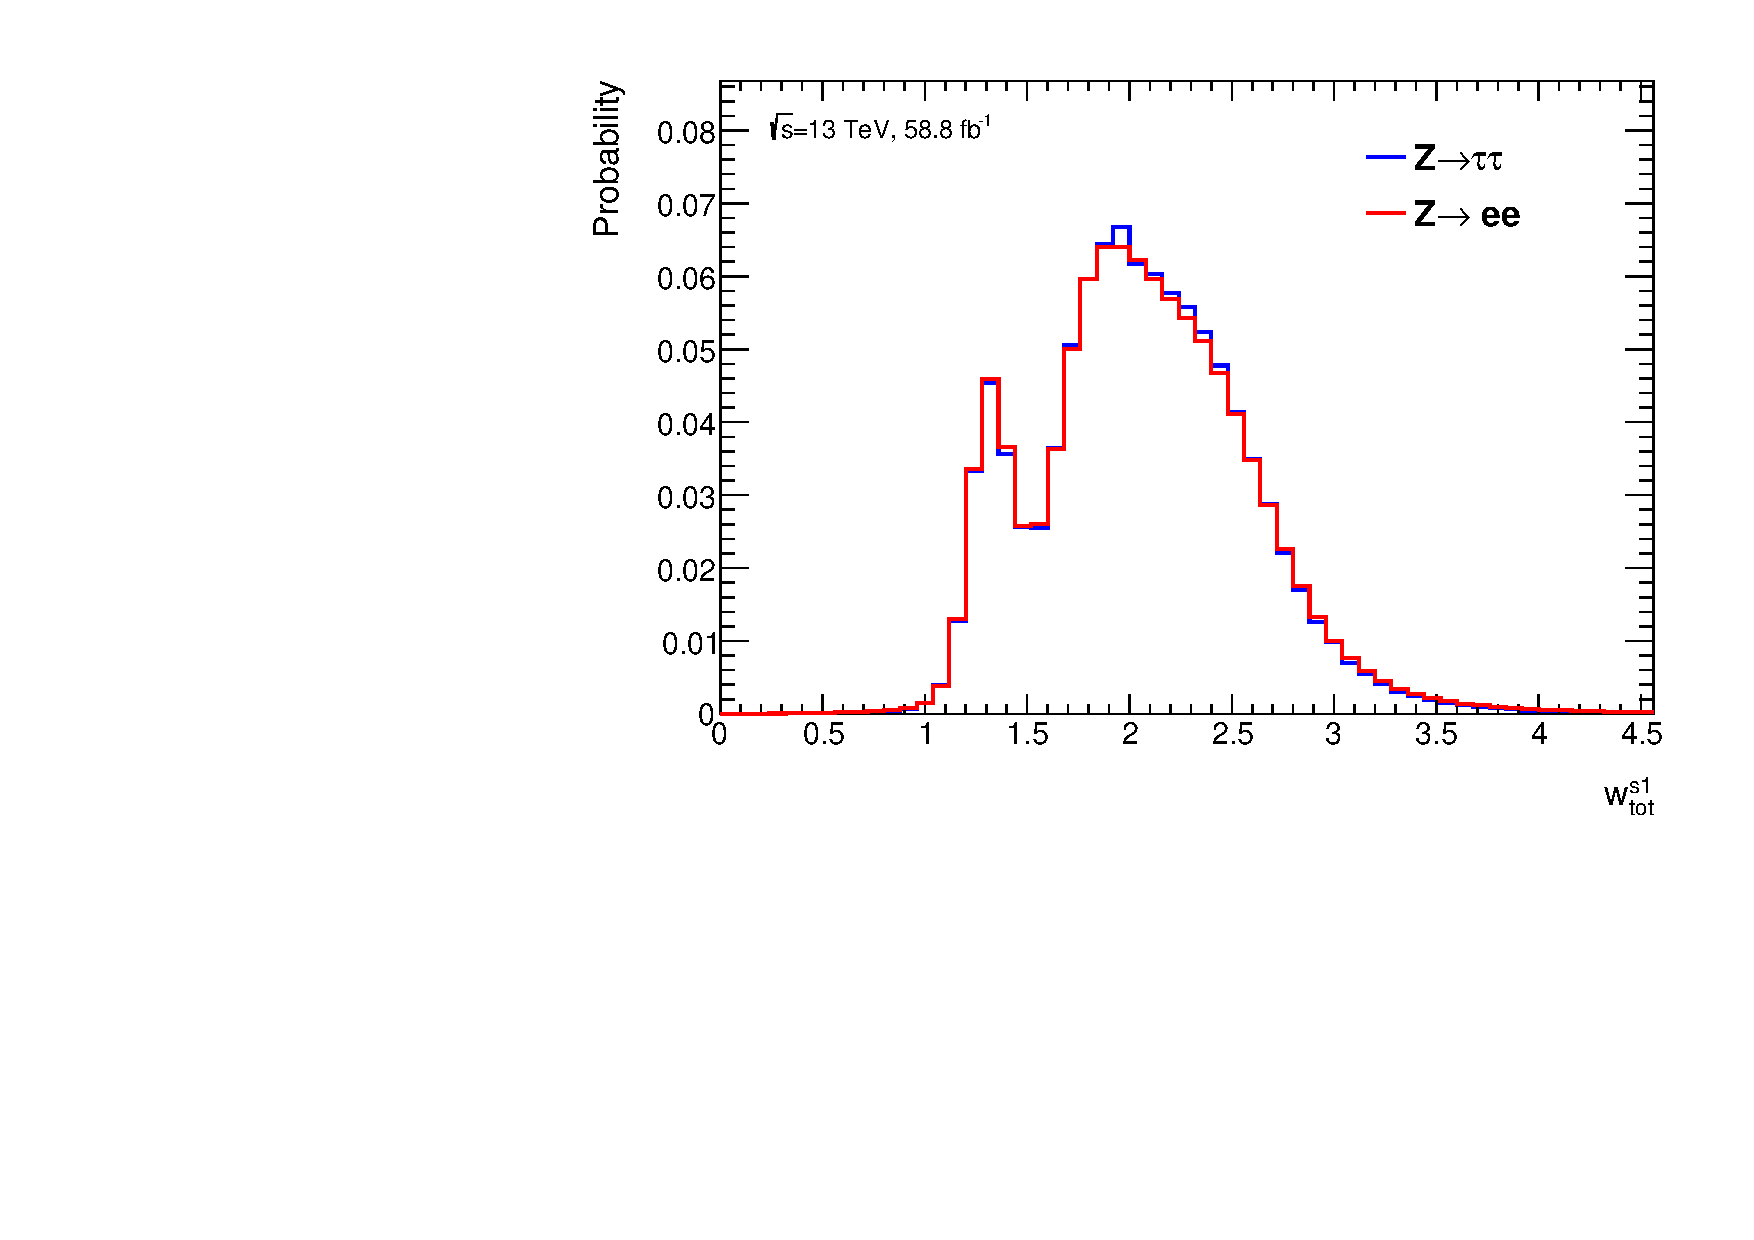
\includegraphics[width=\textwidth]{h_wtots1_Ztautau_comparison.pdf}
      \caption{}
  \end{subfigure}
  \hfill
  \begin{subfigure}[b]{0.45\textwidth}
      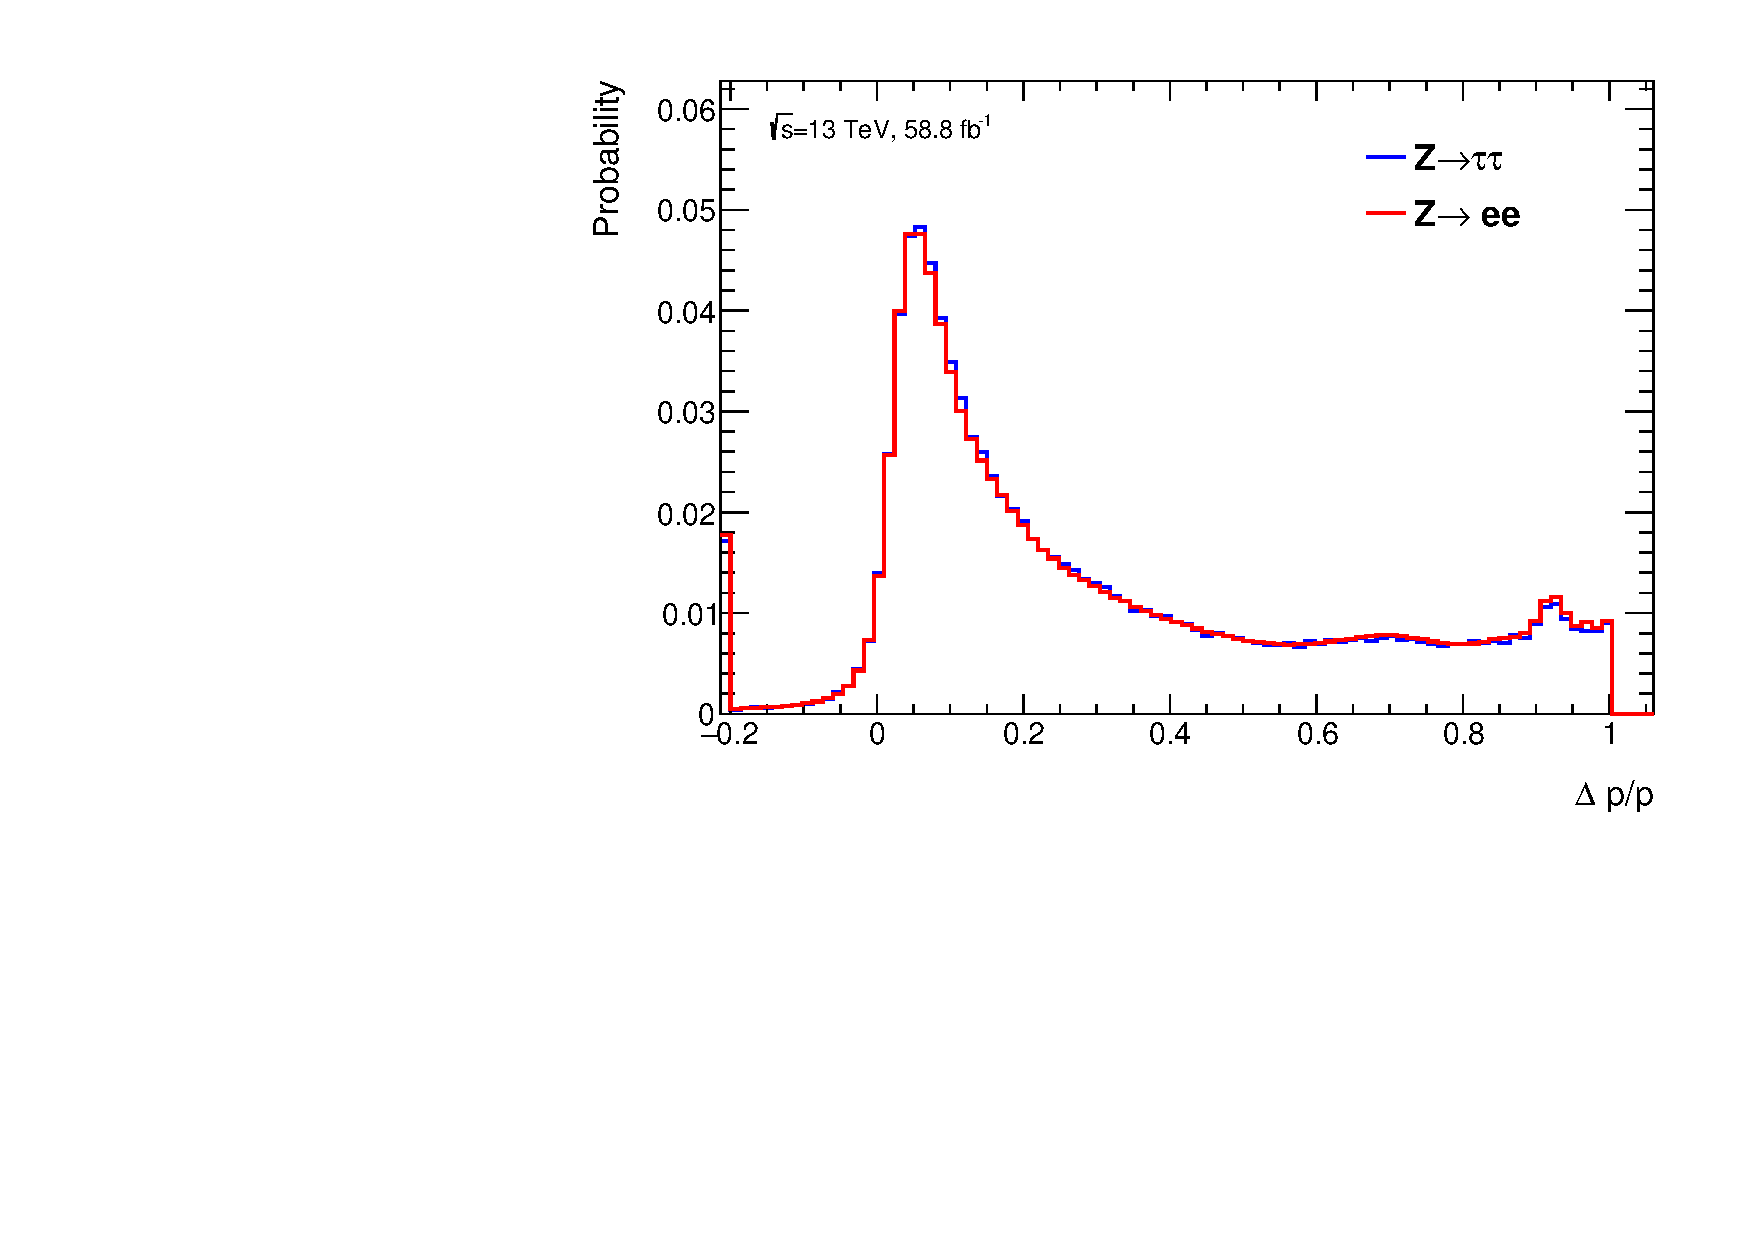
\includegraphics[width=\textwidth]{h_dPOverP_Ztautau_comparison.pdf}
      \caption{}
  \end{subfigure}

  \vspace{0.4cm} % Espacio entre filas

  % ---- Fila 2: una subfigura centrada ----
  \begin{subfigure}[b]{0.6\textwidth}
      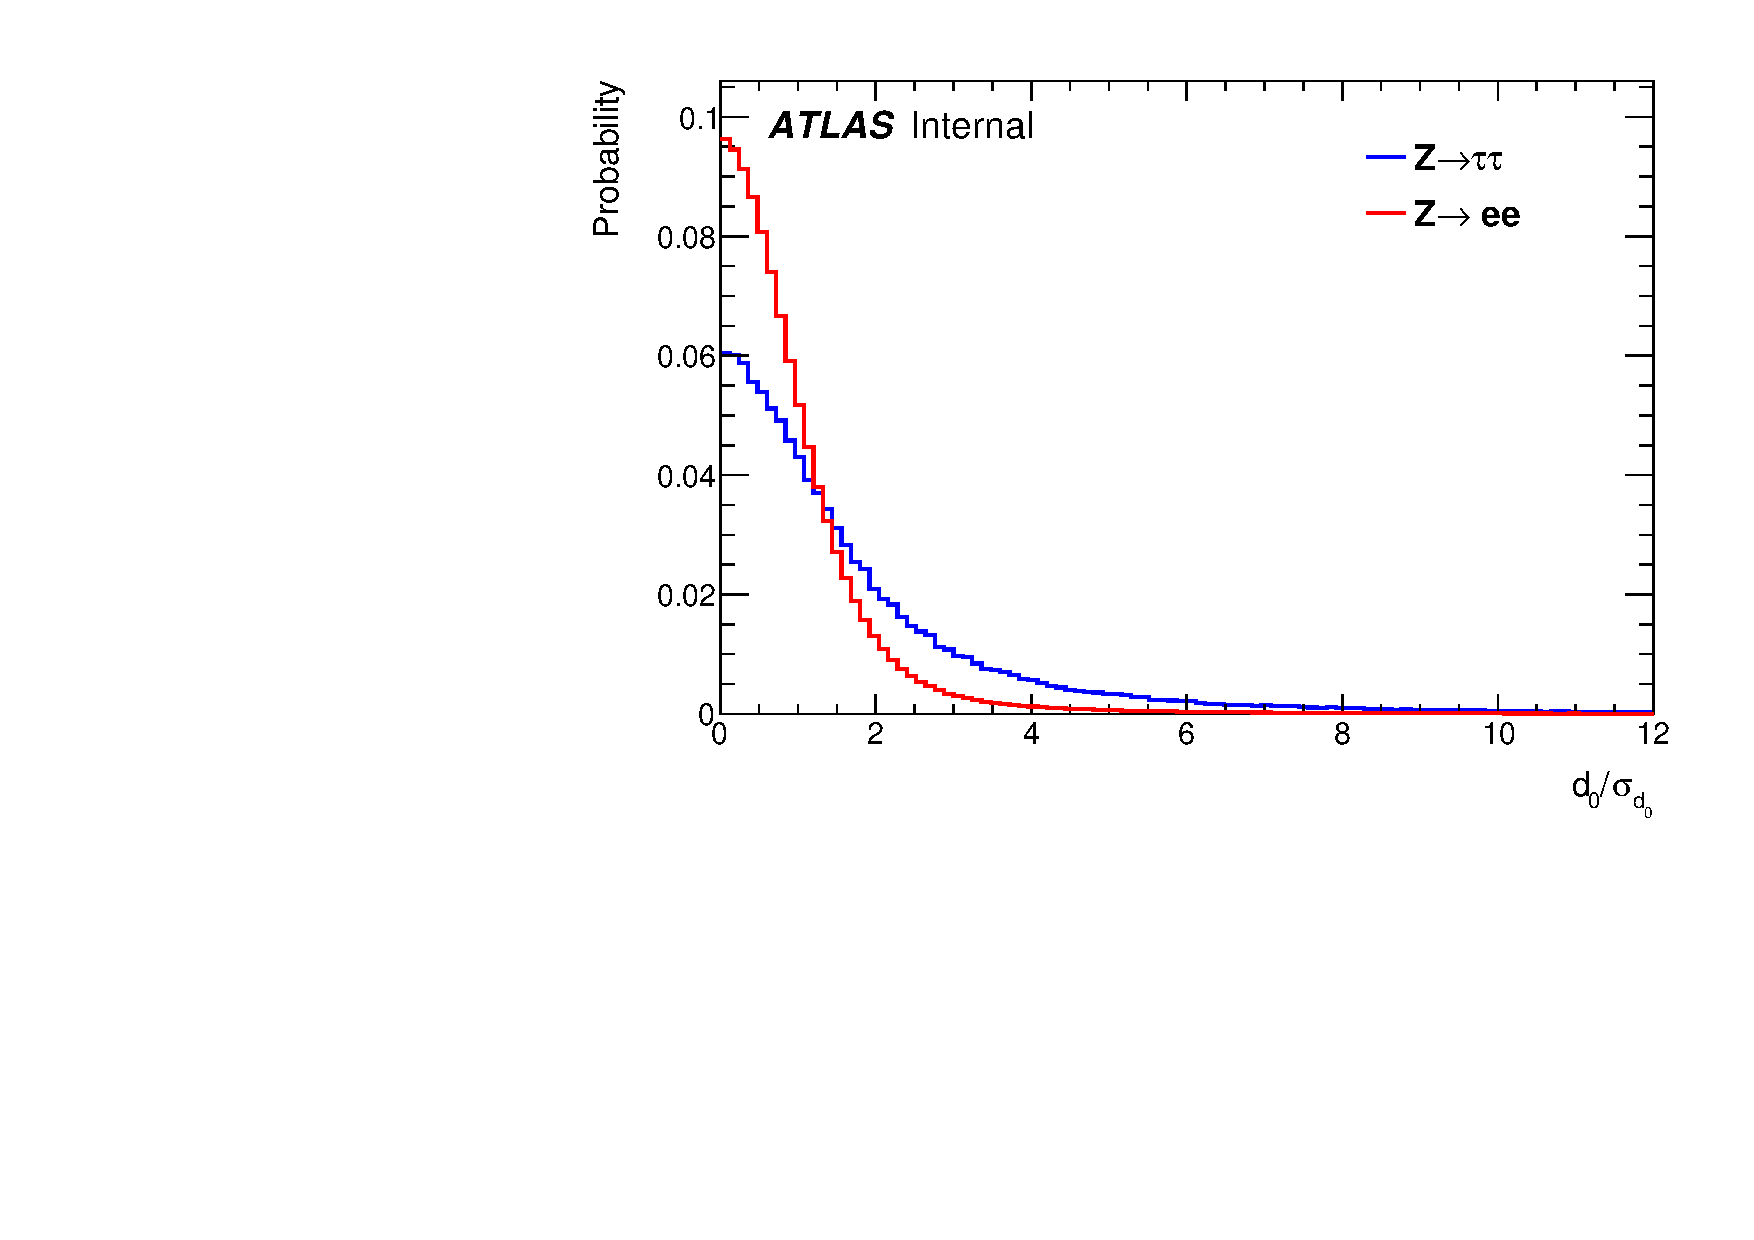
\includegraphics[width=\textwidth]{h_d0Sig_Ztautau_comparison.pdf}
      \caption{}
  \end{subfigure}

  \caption{Comparison of distributions for two calorimeter-based variables (a) and (b), and an impact parameter related one (c), between prompt electrons from $Z \rightarrow ee$ decays and $\tau_{e}$ electrons from $Z \rightarrow \tau\tau$. The definition of these variables is detailed in Table~\ref{table:inputs}.}
  \label{fig:compare}
\end{figure}


A similar situation arises with electrons from Heavy-Flavour decays: although generally treated as background for training purposes, some analyses may require keeping them or applying dedicated rejection techniques. In this context, the class definitions used in this work are optimised for the training of the DNN, but they may need to be reinterpreted depending on the specific analysis requirements.


\subsubsection{Inputs and preprocessing}
%Define which variables are used and why, as well as how we treat them before they're passed through the NN. Hablar obviamente de correction factors, fudging, problems with fudging, correlations and so on.
In order to feed our DNN with the features from the different classes of electron candidates, information left by these particles in almost all ATLAS subdetectors (except the MS) is used, as well as matching information between the tracking systems and energy deposits in the calorimeter. 
In Table~\ref{table:inputs}, all the variables used are listed, along with a brief definition for each of them.

As specified, there are some variables that are not used as input features for training the DNN, but are instead applied as simple rectangular cuts afterwards, in the optimisation step that will be detailed in the next section, since in some specific cases they could provide additional discrimination power. There are also other variables that, in addition to being used for training, are also employed for these rectangular cuts, such as $n_{\text{Si}}$ and $n_{\text{Pixel}}$.

%\renewcommand{\arraystretch}{0.95}
{\scriptsize
\begin{longtable}{p{2.3cm}p{6.5cm}p{1.8cm}p{1.8cm}}
  \caption{Description, name, and usage of the input variables used for the electron identification DNN. For those variables in which it is specified "C" in usage, it means that they are used to perform rectangular cuts as additional requirements when defining the DNN working points. When defining the variables constructed using the second layer of the calorimeter, $3\times3$, $3\times5$, $3\times7$,and $7\times7$ refer to areas of $\Delta \eta \times \Delta \phi$ space in units of $0.025\times0.0245$. Description based on~\cite{dnn_paper}.}\\
  \toprule
  \textbf{Type} & \textbf{Description} & \textbf{Name} & \textbf{Usage} \\
  \midrule
  \endfirsthead
  \midrule
  \endhead
  Hadronic leakage & Ratio of $E_{\text{T}}$ in the first layer of the HCAL to $E_{\text{T}}$ of the EM cluster. & $R_{\text{had1}}$ & DNN \\
   & Ratio of $E_{\text{T}}$ in the HCAL to $E_{\text{T}}$ of the EM cluster. & $R_{\text{had}}$ & DNN \\
  \midrule
  Third layer of EM calorimeter & Ratio of the energy in the third layer to the total energy in the ECAL. & $f_3$ & DNN \\
  \midrule
  First layer of EM calorimeter & Lateral shower width in the second layer of the ECAL. & $w_{\eta2}$ & DNN \\
   & Ratio of the energy in $3{\times}3$ cells in the second layer of the ECAL over the energy in $7{\times}7$ cells centered at the electron cluster position. & $R_{\eta}$ & DNN \\
   & Ratio of the energy in $3{\times}7$ cells in the second layer of the ECAL over the energy in $7{\times}7$ cells centered at the electron cluster position. & $R_{\phi}$ & DNN \\
   & Shower width in the first layer of the ECAL. & $w_{stot}$ & DNN\\
   & Ratio of the energy difference between the maximum energy deposit and the energy deposit in a secondary maximum in the cluster to the sum of these energies in the first layer of the ECAL. & $E_{\text{ratio}}$ & DNN \\
   & Ratio of the energy in the first layer to the total energy in the ECAL. & $f_1$ & DNN \\
  \midrule
  Track conditions & Number of hits in the Pixel detector. & $n_{\text{Pixel}}$ & DNN + C \\
   & Extra hit required in the insertable BLayer. & \texttt{BLayer} & C \\
   & Total number of hits in the Pixel and SCT detectors. & $n_{\text{Si}}$ & DNN + C \\
   & Charged transverse impact parameter relative to the beam-line. & $d_0$ & DNN \\
   & Electron weighted average charge over all associated SCT tracks. & \tiny{\texttt{SCTWeightedCharge}} & DNN \\
   & Significance of transverse impact parameter defined as the ratio of $d_0$ to its uncertainty. & $|d_0/\sigma(d_0)|$ & DNN \\
   & Momentum lost by the track between the perigee and the last measurement point divided by the momentum at perigee. & $\Delta p/p$ & DNN \\
  \midrule
  TRT & Likelihood probability based on transition radiation in the TRT. & \scriptsize{\texttt{TRT PID}} & DNN \\
  \midrule
  Track-cluster matching & $\Delta\eta$ between the cluster position in the first layer and the extrapolated track. & $\Delta\eta_1$ & DNN \\
   & $\Delta\phi$ between the cluster position in the second layer of the ECAL and the momentum-rescaled track. & $\Delta\phi_{\text{res}}$ & DNN \\
   & Ratio of the cluster energy to the track momentum. & $E/p$ & DNN\\
   & Transverse energy of the electron measured by the calorimeter system. & $E_{\text{T}}$ & DNN \\
   & Absolute value of the pseudorapidity of the electron. & $|\eta|$ & DNN \\
  \midrule 
  Reconstruction & Output of an ambiguity resolution algorithm to distinguish objects reconstructed as both electrons and photons. & \scriptsize{\texttt{Amb-type}} & C \\
  \bottomrule
  \label{table:inputs}
\end{longtable}
}
As previously mentioned, the choice of input variables is not exactly the same as the one used to construct the LH discriminant~\cite{Aaboud:2657964}. First of all, the \et and $\eta$ of the electron candidates appear indirectly in the LH construction, since the PDFs are provided in different bins of these variables in order to account for the differences in the kinematic features of the candidates across the various regions of the phase space. Since replicating this binning strategy for the DNN would be computationally expensive, these variables have been instead included as inputs to provide the model with information about the phase space, although, as we will see, they are treated with special care.

Moreover, it has been already mentioned that the number of hits in the main track of our electron candidates is not only used for rectangular cuts, as done in the LH approach, but also as input variables in the training together with other variables like $E/p$ and $w_{\text{stot}}$. 

Most importantly, this strategy allows the usage of highly correlated variables, such as $R_{\text{had1}}$ and $R_{\text{had}}$, which capture, at different levels, the fraction of energy from the EM cluster that leaks into the hadronic calorimeter system. In the LH construction, by definition, only one of these variables can be used, depending on the detector geometry region. In contrast, machine learning algorithms such as DNNs can greatly benefit from input feature correlations, especially in classification tasks where these correlations differ across the various classes.

It is also important to highlight that two variables included in the list are not used in the LH approach nor in the previous version of this DNN~\cite{dnn_paper}. 

The first of these variables is the so-called \texttt{SCTWeightedCharge}, which is defined as:
\begin{equation}
  \texttt{SCTWeightedCharge} = q^{e}\sum_{\text{trk}}\left( q^{\text{trk}}N^{\text{trk}}_{\text{SCT}} \right)/\sum_{\text{trk}} N^{\text{trk}}_{\text{SCT}}
\end{equation}
where $q^{e}$ is the charge of the electron (as given by its primary track), $N^{\text{trk}}_{\text{SCT}}$ is the number of hits in the SCT for a given track associated to the electron, and $q^{\text{trk}}$ is the charge associated to that track. This variable can be interpreted as the electron charge weighted over all tracks associated with the electron, beyond the primary one. By construction, it takes a value of one if the electron has only one associated track. However, in cases where multiple tracks are associated to the same electron candidate, the value may differ from one, which is typically more likely when the candidate corresponds to a charge-flip electron.

The second variable is the so-called charged impact parameter, $q \times d_{0}$, which replaces the $d_{0}$ variable used previously.

The main interest of these two variables lies in their discriminating power for rejecting charge-flip electrons against prompt electrons candidates with correctly identified charge~\cite{carnelli}. This provides the DNN with an additional potential to identify this specific class of electrons. This feature will be discussed in more detail in a later section.

\paragraph{Shower-shape variables corrections} \mbox{}\\
\\
It is worth starting by defining what a shower-shape variable is in this context. As the name suggests, these are the variables already described in Table~\ref{table:inputs} that characterise the shape of the electromagnetic shower left by the electron candidates in the calorimeter system.

The main issue that arises here is that, in order to train our DNN and ensure that it performs well when applied to real data, we ideally want the distributions of the input variables for simulated electrons to closely resemble those of real electrons coming from data. However, due to imperfections in the detector modelling, the disagreement between MC simulations and data can be too large especially for those variables involving calorimeter signal readouts. % (such as energy leakage due to undesired connections between LAr cells, commonly referred to as \textit{cross-talk}).

Corrections are therefore derived for these shower-shape variables in cases where the differences between data and MC are too significant. These corrections are based on individual affine transformations applied in bins of $E_{\text{T}}$ and $\eta$, such that the mean of the distribution being stretched and/or its width shifted, depending on the severity of the discrepancy.

The corrections are derived by comparing the distributions evaluated for \zee electron candidates extracted from data and MC simulations using a simple tag-and-probe technique. The transformation parameters are obtained by minimising the $\chi^2$ between the two distributions. More details can be found in Ref.~\cite{Aaboud:2657964}, but an example of the application of these corrections can be seen in Figure~\ref{fig:corrected} for the variables $f_{3}$ and $R_{\text{had}}$.


\begin{figure}[htbp]
  \centering
  \begin{subfigure}[b]{0.48\textwidth}
      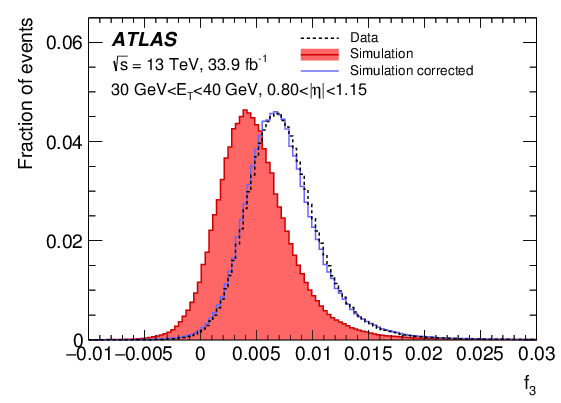
\includegraphics[width=\textwidth]{id_datamcf3.png}
      \caption{}
  \end{subfigure}
  \hfill
  \begin{subfigure}[b]{0.48\textwidth}
      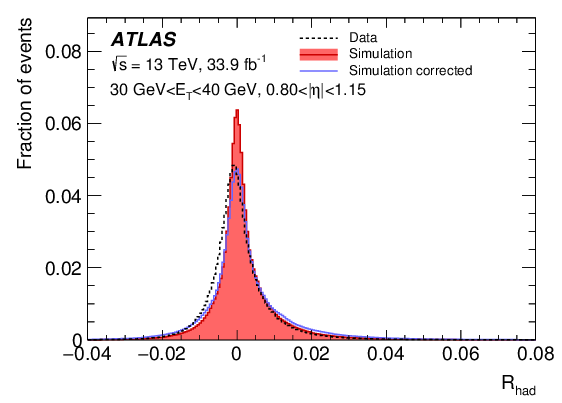
\includegraphics[width=\textwidth]{id_datamcrhad.png}
      \caption{}
  \end{subfigure}
  \hfill
  \caption{Comparison of (a)$f_{3}$ and (b)$R_{\text{had}}$ shower-shape distributions for data and MC electrons with and without corrections applied, within certain $E_{\text{T}}$ and $\eta$ bins: $30 < E_{\text{T}} < 40$~GeV and $0.8<|\eta|<1.15$. Source in Ref.~\cite{Aaboud:2657964}}
  \label{fig:corrected}
\end{figure}

It can be observed that, in the case of $f_3$, the simulated values of this variable are centred around a mean value that is slightly shifted with respect to the real data distribution. Therefore, in this case, a small shift in the mean of the distribution would be sufficient. 
For $R_{\text{had}}$, however, it is also evident that in order to match the data values, it is necessary not only to shift the distribution but also to broaden it slightly around the mean value, applying a correction to the width as well.

%SHIFT&STRETCH Y QUE HAY OTRO QUE SE USO QUE NO VALE PARA DNN POR LAS CORRELACIONES Y PONER PLOTS DE CORRELACIONES Y DECIR QUE SE CONSERVAN GUAY ;)
This correction method, often referred to as \textit{fudging} in this context, is known as the \textit{Shift}$\&$\textit{Stretch} approach. Other strategies exist to address discrepancies between data and MC simulations, such as the \textit{Gaussian Smearing} approach, which assumes that the noise-like imperfections introduced by the calorimeter can be incorporated into MC simulations through Gaussian approximations~\cite{Puddefoot:2797826}.

This \textit{Gaussian Smearing} approach was used to correct the PDFs employed in the construction of the LH discriminant using reprocessed Run-2 data. However, it cannot be applied to the DNN input variables. The reason is that these Gaussian corrections introduce artificial correlations in the input distributions, which ultimately degrade the performance of the DNN. Unlike the LH method, which is designed to be robust against such effects, DNNs rely on the preservation of meaningful correlations between features.

The \textit{Shift}$\&$\textit{Stretch} method, on the other hand, applies simple affine transformations that better preserve these correlations. This can be seen in Figure~\ref{fig:correlations}, where the correlation matrices between input variables are shown for MC simulations before and after corrections, and for collision data.

\begin{figure}[htbp]
  \centering
  \begin{subfigure}[b]{0.45\textwidth}
      \centering
      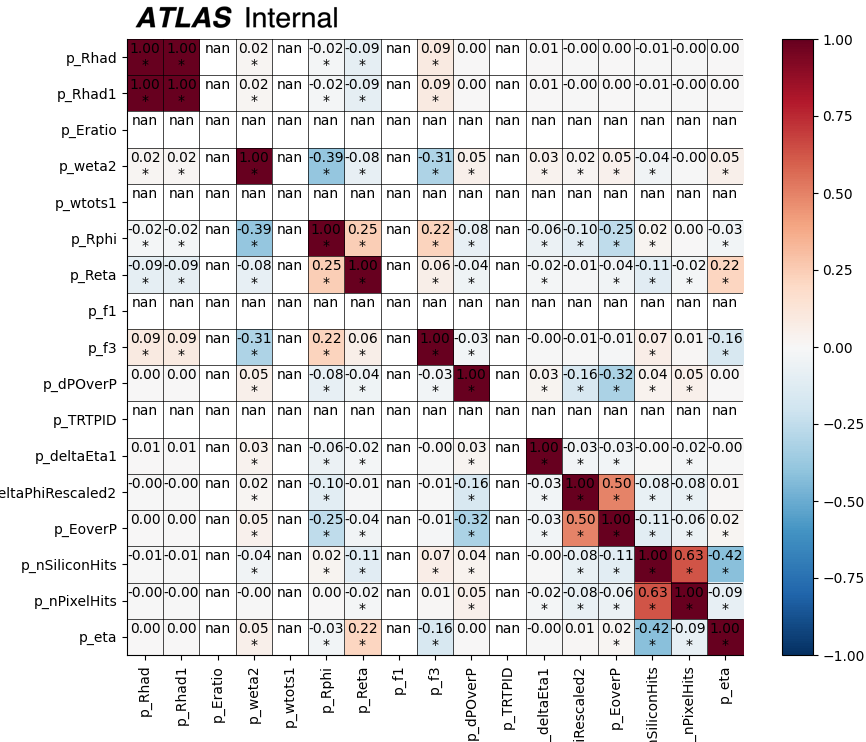
\includegraphics[width=\textwidth]{correlation_matrix_nofudge_eta_gt241_f1.png}
      \caption{MC simulation without corrections}
      \label{fig:corr_nominal}
  \end{subfigure}
  \hfill
  \begin{subfigure}[b]{0.45\textwidth}
      \centering
      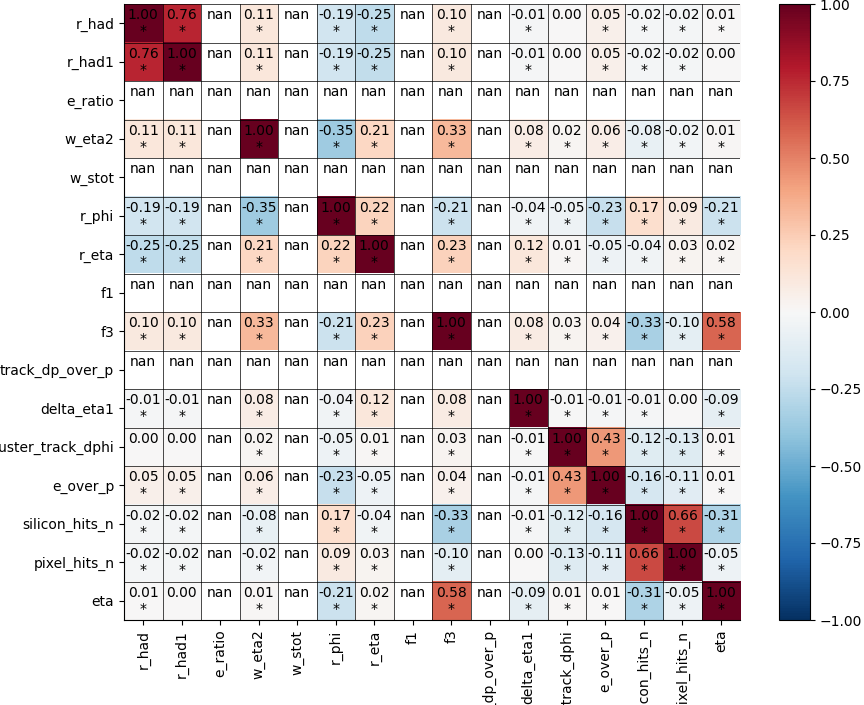
\includegraphics[width=\textwidth]{correlation_matrix_data18_eta_gt241_f1.png}
      \caption{Data}
      \label{fig:corr_data}
  \end{subfigure}
  \vspace{0.4cm}
  \begin{subfigure}[b]{0.45\textwidth}
      \centering
      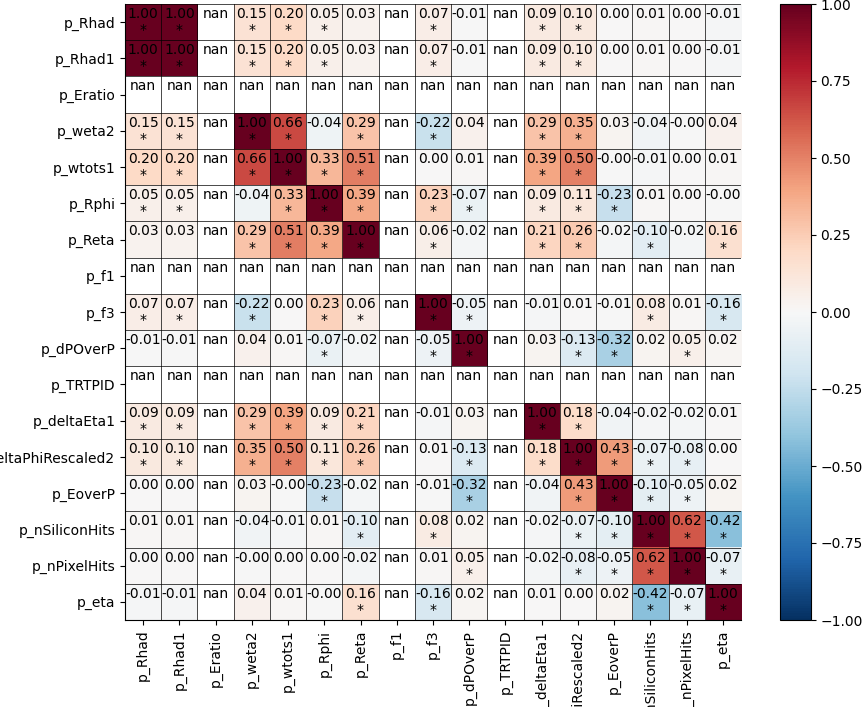
\includegraphics[width=\textwidth]{correlation_matrix_newtool_eta_gt241_f1.png}
      \caption{MC simulation with Gaussian Smearing}
      \label{fig:corr_smearing}
  \end{subfigure}
  \hfill
  \begin{subfigure}[b]{0.45\textwidth}
      \centering
      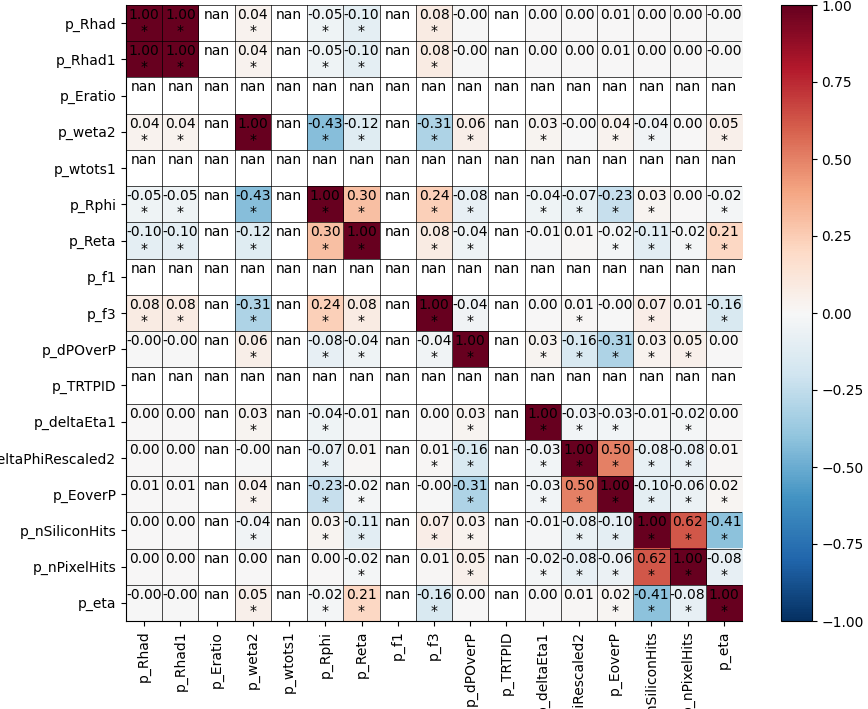
\includegraphics[width=\textwidth]{correlation_matrix_oldtool_newderivedFFs_eta_gt241_f1.png}
      \caption{MC simulation with Shift\&Stretch}
      \label{fig:corr_shiftstretch}
  \end{subfigure}
  \caption{Comparison of input variable correlations for different correction strategies. Only electrons from the end-cap region ($|\eta|>2.41$) and with $f_{1}=0$ are selected since are more representative of this discrepancy between approaches.}
  \label{fig:correlations}
\end{figure}

\paragraph{Preprocessing} \mbox{}\\
\\
Before proceeding to the training of our DNN, it is important to remember that different physical processes have been used to populate the various electron candidate classes we defined. Consequently, the $E_{\text{T}}$ distribution can vary significantly among classes. For instance, most prompt electrons from $Z \to e^{+}e^{-}$ decays will have $E_{\text{T}} \approx 45$~GeV, corresponding to half of the $Z$-boson mass. This could introduce significant biases and degrade the DNN’s performance, as discussed in Section~\ref{dnn:preprocessing}.
To prevent the network from distinguishing classes based solely on $E_{\text{T}}$ and $\eta$, these input distributions need to be harmonised across all six classes. This is achieved through a combination of downsampling and reweighting.

First, to limit the statistical imbalance, the prompt electron sample is downsampled. Prompt candidates are randomly removed in $E_{\text{T}}$ bins so that, within each bin, their number does not exceed five times the number of background candidates. This effectively reduces the prominent peak at 45~GeV, as illustrated in Figure~\ref{fig:et_downsampling}. Due to limited statistics, no downsampling is applied to the charge-flip class, even though a similar peak is present.

Once downsampling is applied, weights are derived to reweight the $E_{\text{T}}$ and $\eta$ distributions independently for each class. These weights are then combined by multiplying the two, assuming no strong correlation between $E_{\text{T}}$ and $\eta$. After reweighting, all distributions are normalised so that the total weight per class remains constant. The resulting harmonised distributions for $E_{\text{T}}$ and $\eta$ are shown in Figures~\ref{fig:et_reweighted} and~\ref{fig:eta_reweighted}.

The $\eta$ reweighting aims for a flat distribution, while for $E_{\text{T}}$, a shape resembling the Light-Flavour hadron class from the \ttbar sample is targeted, featuring a flat region up to 15~GeV followed by a falling slope. This approach reduces the bias efficiently while preserving classification performance. Some residual discrepancies may remain due to small final correlations between $E_{\text{T}}$ and $\eta$, especially for the charge-flip class. While a 2D reweighting could mitigate this, it is avoided due to limited statistics at high $E_{\text{T}}$.

Finally, to equalise the total statistical weight across classes, an additional scaling factor is applied per class after reweighting. This factor ensures that all classes contribute equally in terms of weight, while keeping the global sum of weights unchanged. An example of this normalization is shown in the case of the $E_{\text{T}}$ distribution in Figure~\ref{fig:et_classWeighted}.

\begin{figure}[htbp]
  \centering
  \begin{subfigure}[b]{0.48\textwidth}
      \centering
      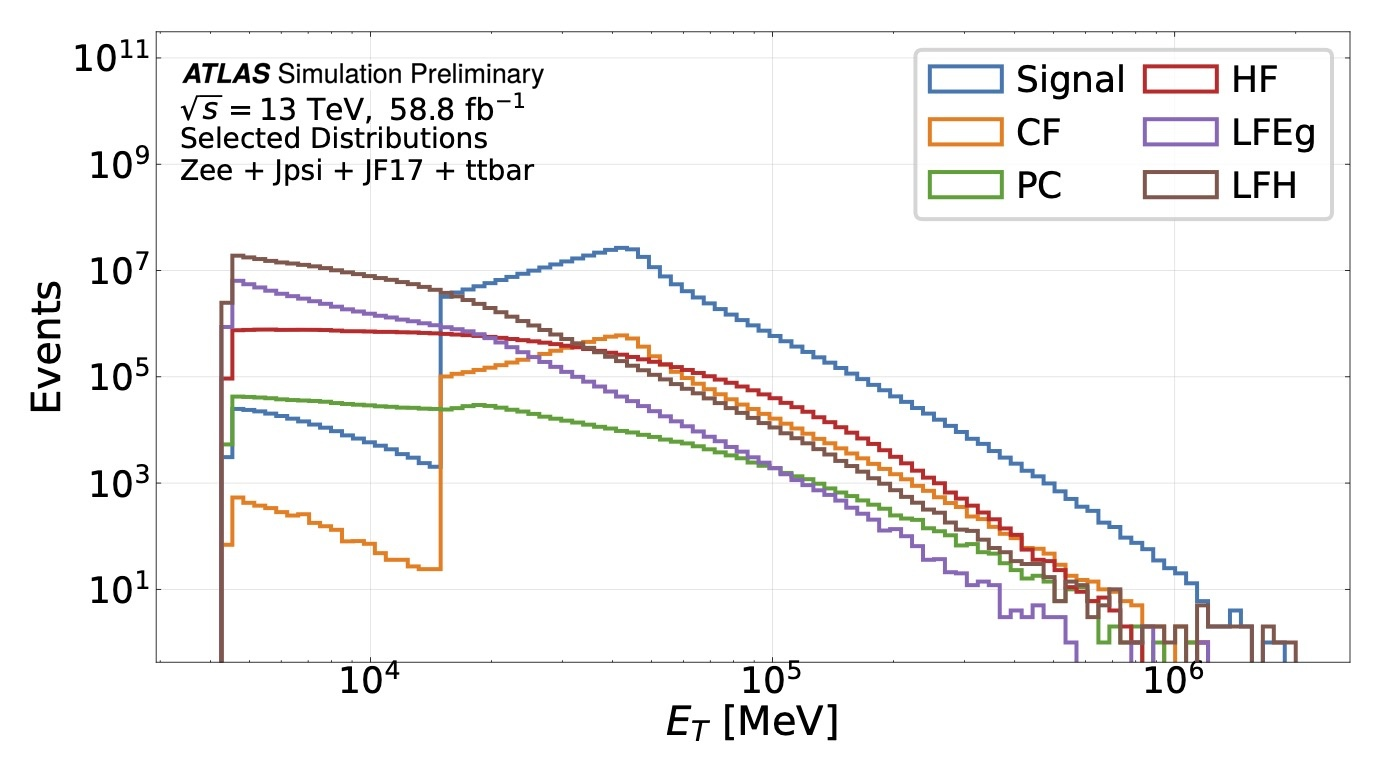
\includegraphics[width=\textwidth]{selection_MultiClass_Et_train.jpg}
      \caption{$E_{\text{T}}$ at selection level}
      \label{fig:et_selection}
  \end{subfigure}
  \hfill
  \begin{subfigure}[b]{0.48\textwidth}
      \centering
      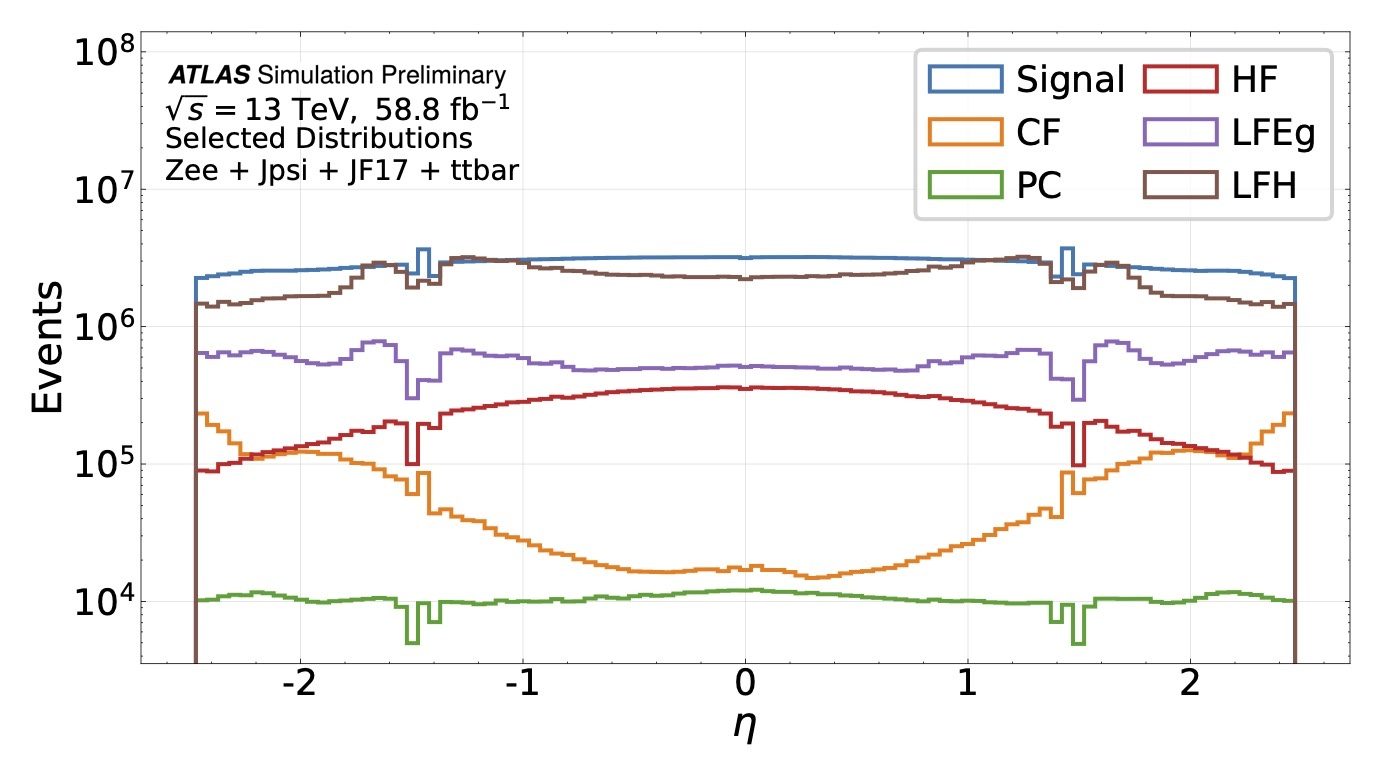
\includegraphics[width=\textwidth]{selection_MultiClass_Eta_train.jpg}
      \caption{$\eta$ at selection level}
      \label{fig:eta_selection}
  \end{subfigure}
  \vspace{0.4cm}
  \begin{subfigure}[b]{0.48\textwidth}
      \centering
      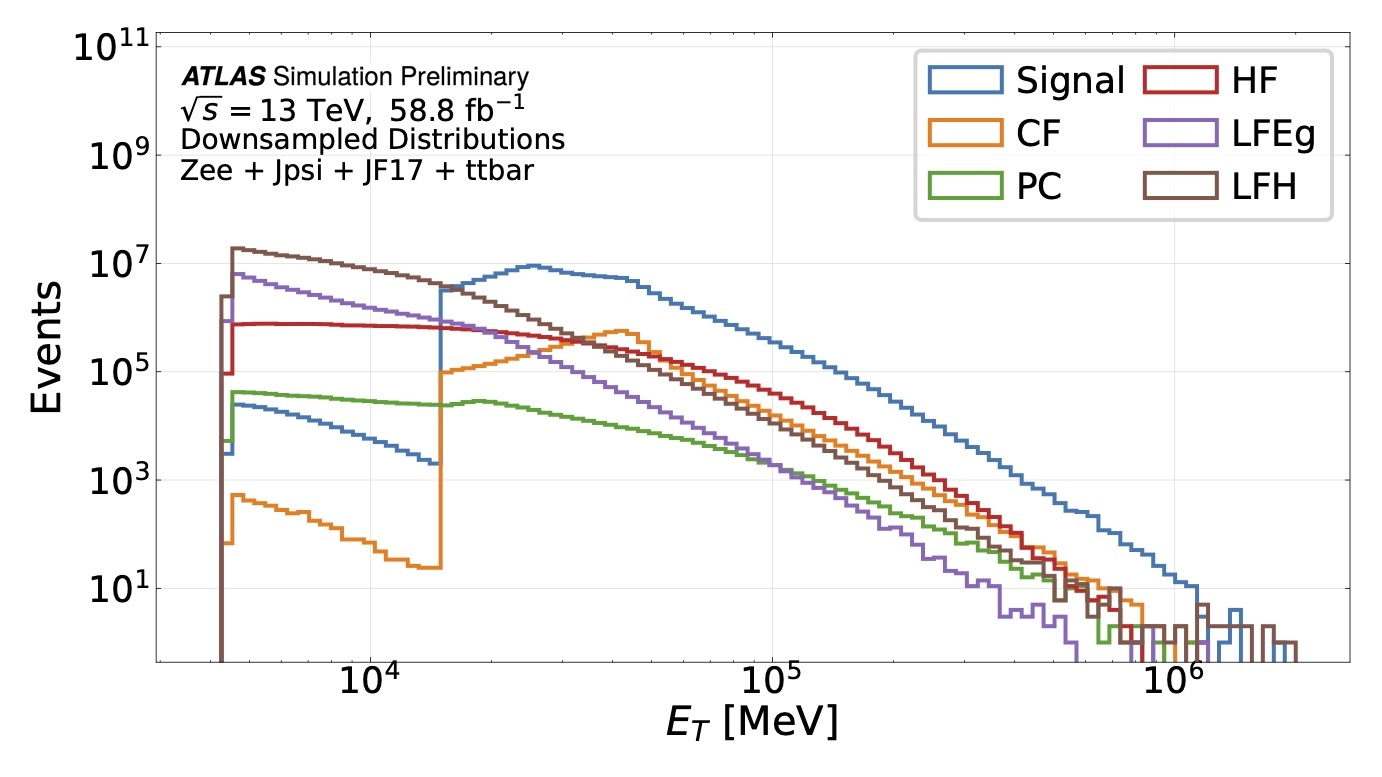
\includegraphics[width=\textwidth]{downsampled_MultiClass_Et_train.jpg}
      \caption{$E_{\text{T}}$ downsampled}
      \label{fig:et_downsampling}
  \end{subfigure}
  \hfill
  \begin{subfigure}[b]{0.48\textwidth}
      \centering
      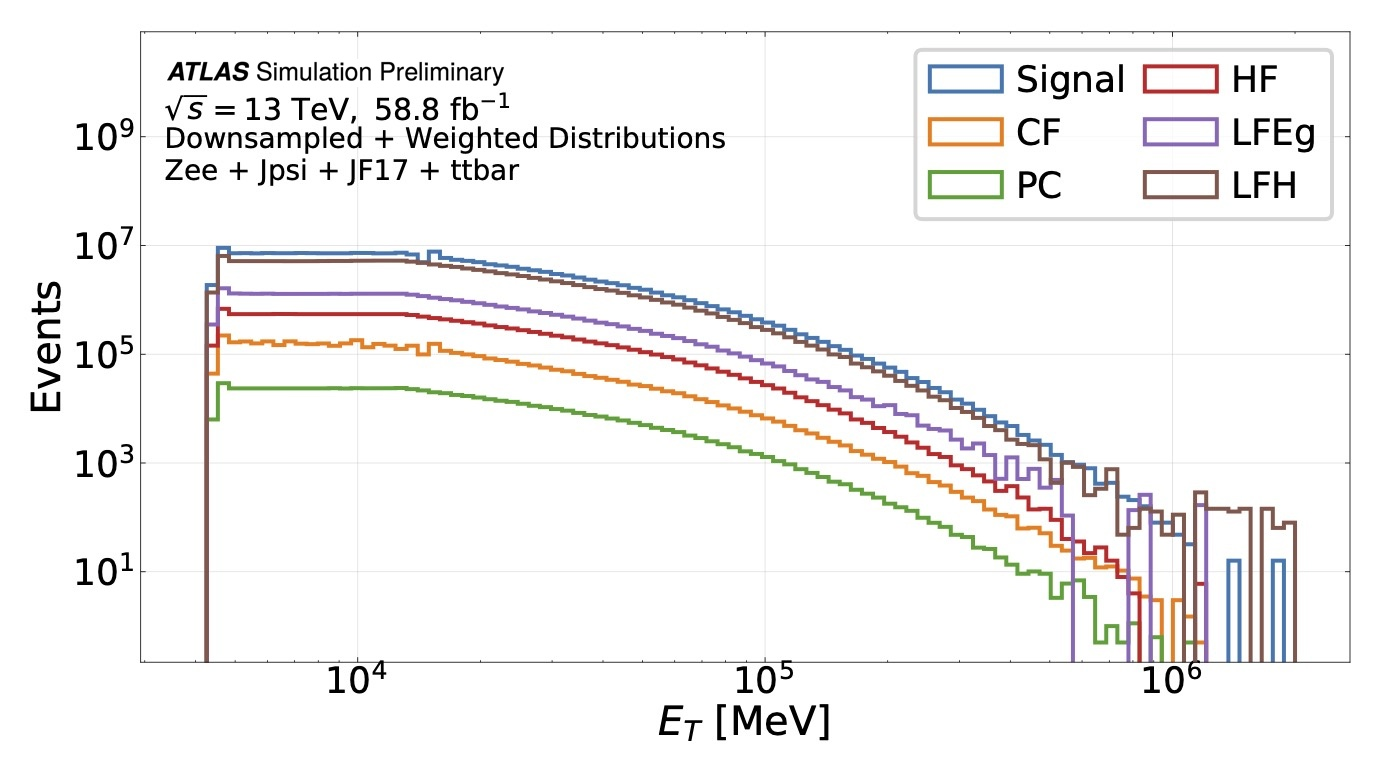
\includegraphics[width=\textwidth]{weighted_MultiClass_Et_train.jpg}
      \caption{$E_{\text{T}}$ downsampled and weighted}
      \label{fig:et_reweighted}
  \end{subfigure}
  \vspace{0.4cm}
  \begin{subfigure}[b]{0.48\textwidth}
      \centering
      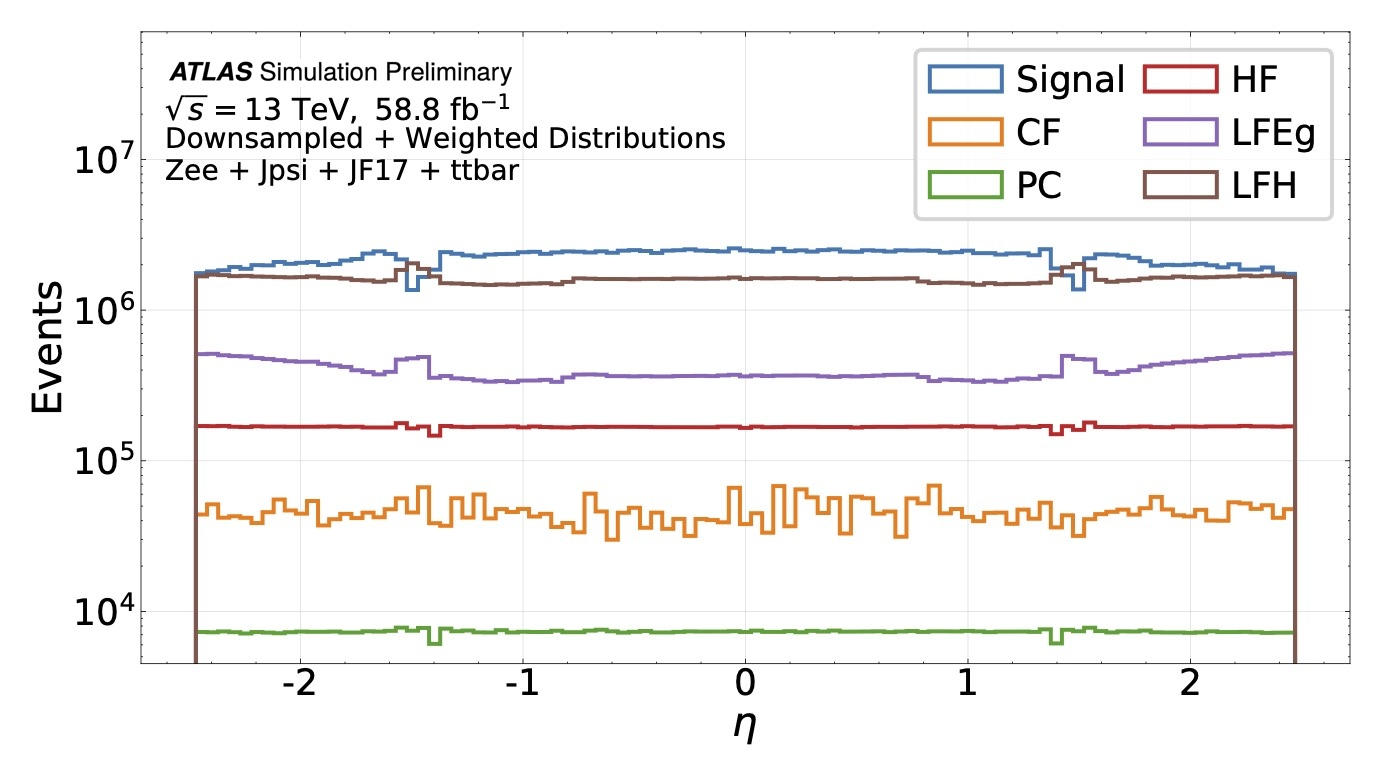
\includegraphics[width=\textwidth]{weighted_MultiClass_Eta_train.jpg}
      \caption{$|\eta|$ weighted}
      \label{fig:eta_reweighted}
  \end{subfigure}
  \hfill
  \begin{subfigure}[b]{0.48\textwidth}
      \centering
      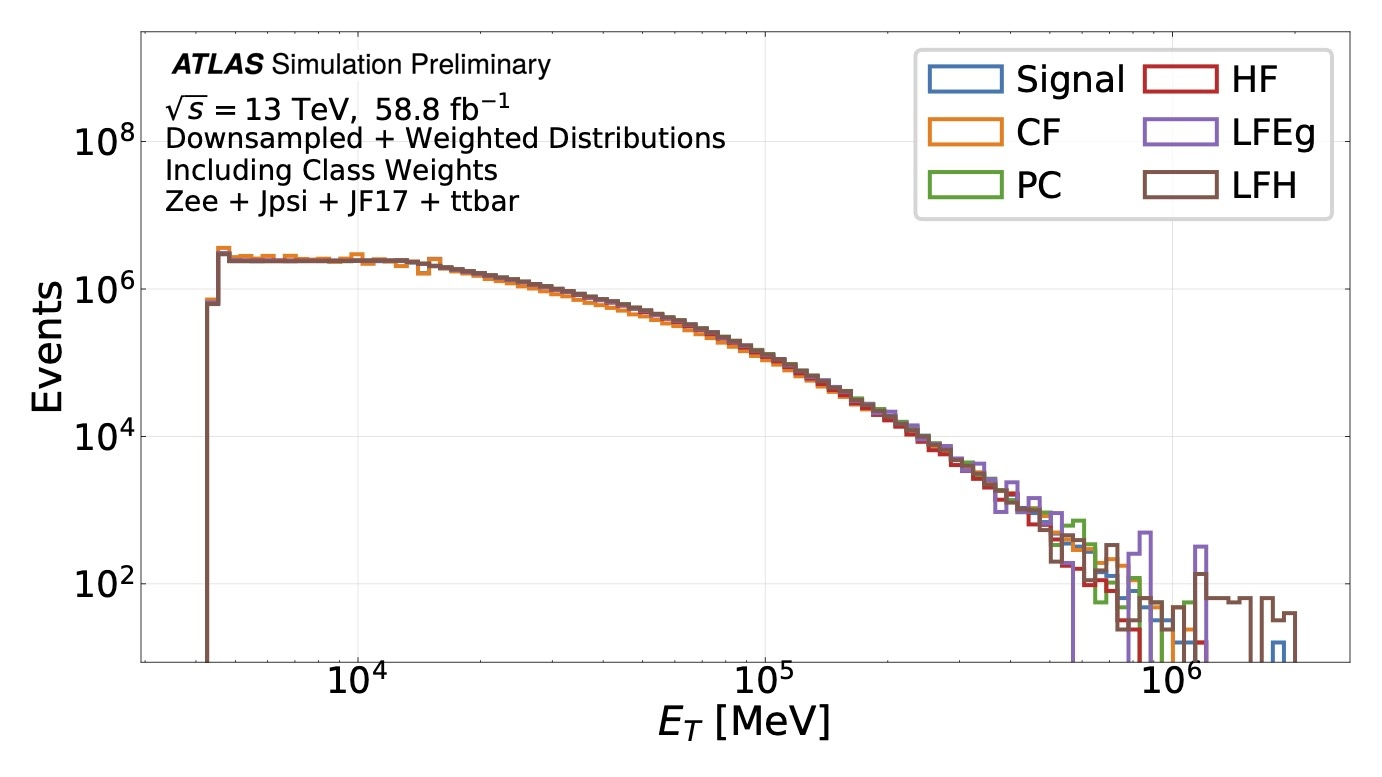
\includegraphics[width=\textwidth]{classWeighted_MultiClass_Et_train.jpg}
      \caption{$E_{\text{T}}$ class-weighted }
      \label{fig:et_classWeighted}
  \end{subfigure}
  \caption{Distributions of $E_{\text{T}}$ and $|\eta|$ at electrons' selection level, (a) and (b), $E_{\text{T}}$ after applying downsampling (c) and kinematic reweighting (d), $\eta$ after flattening reweighting (e), and finally $E_{\text{T}}$ after applying also weights making all the classes equiprobable (f).}
  \label{fig:et_eta_reweighting}
\end{figure}

% Requires: \usepackage{subcaption}
% Nota: un único entorno figure no puede partirse entre páginas.
% Para que continúe en la siguiente, usamos \ContinuedFloat en una segunda figura.

% --- Parte 1 (filas 1–4) ---
\begin{figure}[htbp]
  \centering

  % Row 1
  \begin{subfigure}[b]{0.47\textwidth}
    \centering
    \includegraphics[width=\linewidth]{normalized_weighted_distributions/weighted_Multiclass_rhad1_train.pdf}
    \caption{$R_{\text{had1}}$}
    \label{fig:input1}
  \end{subfigure}\hfill
  \begin{subfigure}[b]{0.47\textwidth}
    \centering
    \includegraphics[width=\linewidth]{normalized_weighted_distributions/weighted_Multiclass_rhad_train.pdf}
    \caption{$R_{\text{had}}$}
    \label{fig:input2}
  \end{subfigure}

  \vspace{0.45cm}

  % Row 2
  \begin{subfigure}[b]{0.47\textwidth}
    \centering
    \includegraphics[width=\linewidth]{normalized_weighted_distributions/weighted_Multiclass_f3_train.pdf}
    \caption{$f_3$}
    \label{fig:input3}
  \end{subfigure}\hfill
  \begin{subfigure}[b]{0.47\textwidth}
    \centering
    \includegraphics[width=\linewidth]{normalized_weighted_distributions/weighted_Multiclass_weta2_train.pdf}
    \caption{$w_{\eta2}$}
    \label{fig:input4}
  \end{subfigure}

  \vspace{0.45cm}

  % Row 3
  \begin{subfigure}[b]{0.47\textwidth}
    \centering
    \includegraphics[width=\linewidth]{normalized_weighted_distributions/weighted_Multiclass_reta_train.pdf}
    \caption{$R_{\eta}$}
    \label{fig:input5}
  \end{subfigure}\hfill
  \begin{subfigure}[b]{0.47\textwidth}
    \centering
    \includegraphics[width=\linewidth]{normalized_weighted_distributions/weighted_Multiclass_rphi_train.pdf}
    \caption{$R_{\phi}$}
    \label{fig:input6}
  \end{subfigure}

  \vspace{0.45cm}

  % Row 4
  \begin{subfigure}[b]{0.47\textwidth}
    \centering
    \includegraphics[width=\linewidth]{normalized_weighted_distributions/weighted_Multiclass_wtots1_train.pdf}
    \caption{$w_{stot}$}
    \label{fig:input7}
  \end{subfigure}\hfill
  \begin{subfigure}[b]{0.47\textwidth}
    \centering
    \includegraphics[width=\linewidth]{normalized_weighted_distributions/weighted_Multiclass_eratio_train.pdf}
    \caption{$E_{\text{ratio}}$}
    \label{fig:input8}
  \end{subfigure}

  \label{fig:dnn_inputs_distributions}
\end{figure}

% --- Parte 2 (filas 5–8), continúa la numeración y el caption de la figura anterior ---
\begin{figure}[htbp]\ContinuedFloat
  \centering

  % Row 5
  \begin{subfigure}[b]{0.47\textwidth}
    \centering
    \includegraphics[width=\linewidth]{normalized_weighted_distributions/weighted_Multiclass_f1_train.pdf}
    \caption{$f_1$}
    \label{fig:input9}
  \end{subfigure}\hfill
  \begin{subfigure}[b]{0.47\textwidth}
    \centering
    \includegraphics[width=\linewidth]{normalized_weighted_distributions/weighted_Multiclass_npixel_train.pdf}
    \caption{$n_{\text{Pixel}}$}
    \label{fig:input11}
  \end{subfigure}

  \vspace{0.45cm}

  % Row 6
  \begin{subfigure}[b]{0.47\textwidth}
    \centering
    \includegraphics[width=\linewidth]{normalized_weighted_distributions/weighted_Multiclass_nsilicon_train.pdf}
    \caption{$n_{\text{Si}}$}
    \label{fig:input12}
  \end{subfigure}\hfill
  \begin{subfigure}[b]{0.47\textwidth}
    \centering
    \includegraphics[width=\linewidth]{normalized_weighted_distributions/weighted_Multiclass_TRTPID_train.pdf}
    \caption{TRT PID}
    \label{fig:input18}
  \end{subfigure}

  \vspace{0.45cm}

  % Row 7
  \begin{subfigure}[b]{0.47\textwidth}
    \centering
    \includegraphics[width=\linewidth]{normalized_weighted_distributions/weighted_Multiclass_d0sig_train.pdf}
    \caption{$|d_0/\sigma(d_0)|$}
    \label{fig:input16}
  \end{subfigure}\hfill
  \begin{subfigure}[b]{0.47\textwidth}
    \centering
    \includegraphics[width=\linewidth]{normalized_weighted_distributions/weighted_Multiclass_qd0_train.pdf}
    \caption{$q \times d_0$}
    \label{fig:input14}
  \end{subfigure}

  \vspace{0.45cm}

  % Row 8
  \begin{subfigure}[b]{0.47\textwidth}
    \centering
    \includegraphics[width=\linewidth]{normalized_weighted_distributions/weighted_Multiclass_sctweightedcharge_train.pdf}
    \caption{\texttt{SCTWeightedCharge}}
    \label{fig:input15}
  \end{subfigure}\hfill
  \begin{subfigure}[b]{0.47\textwidth}
    \centering
    \includegraphics[width=\linewidth]{normalized_weighted_distributions/weighted_Multiclass_dPoverP_train.pdf}
    \caption{$\Delta p/p$}
    \label{fig:input17}
  \end{subfigure}
  \caption{Distributions of all the input variables used for DNN training, after preprocessing and reweighting procedures. Only the training subset of the simulated electrons is used to produce these plots.}

  % No ponemos caption aquí: \ContinuedFloat mantiene el caption y la etiqueta de \ref{fig:dnn_inputs_distributions}
\end{figure}


The distributions of all input variables after the application of these modifications (except the class-reweighting) can be found in Figure~\ref{fig:dnn_inputs_distributions}. However, there is still one last step before passing all the inputs distributions through the DNN, which is the transformation of all of them to uniform distributions between zero and one, using empirical quantiles as explained in Section~\ref{dnn:preprocessing}. This action facilitates the training of the neural network and speeds up the different steps in the optimization.
Figure~\ref{fig:transformed} illustrates the impact of this transformation on the $R_{\text{had}}$ variable, taken from Ref.~\cite{dnn_paper}. The plot displays the full distribution together with the individual contributions from prompt electrons and Light-Flavour hadrons. After applying the transformation, the overall distribution becomes uniform within the $[0,1]$ interval.

\begin{figure}[htbp]
  \centering
  \begin{subfigure}[b]{0.45\textwidth}
      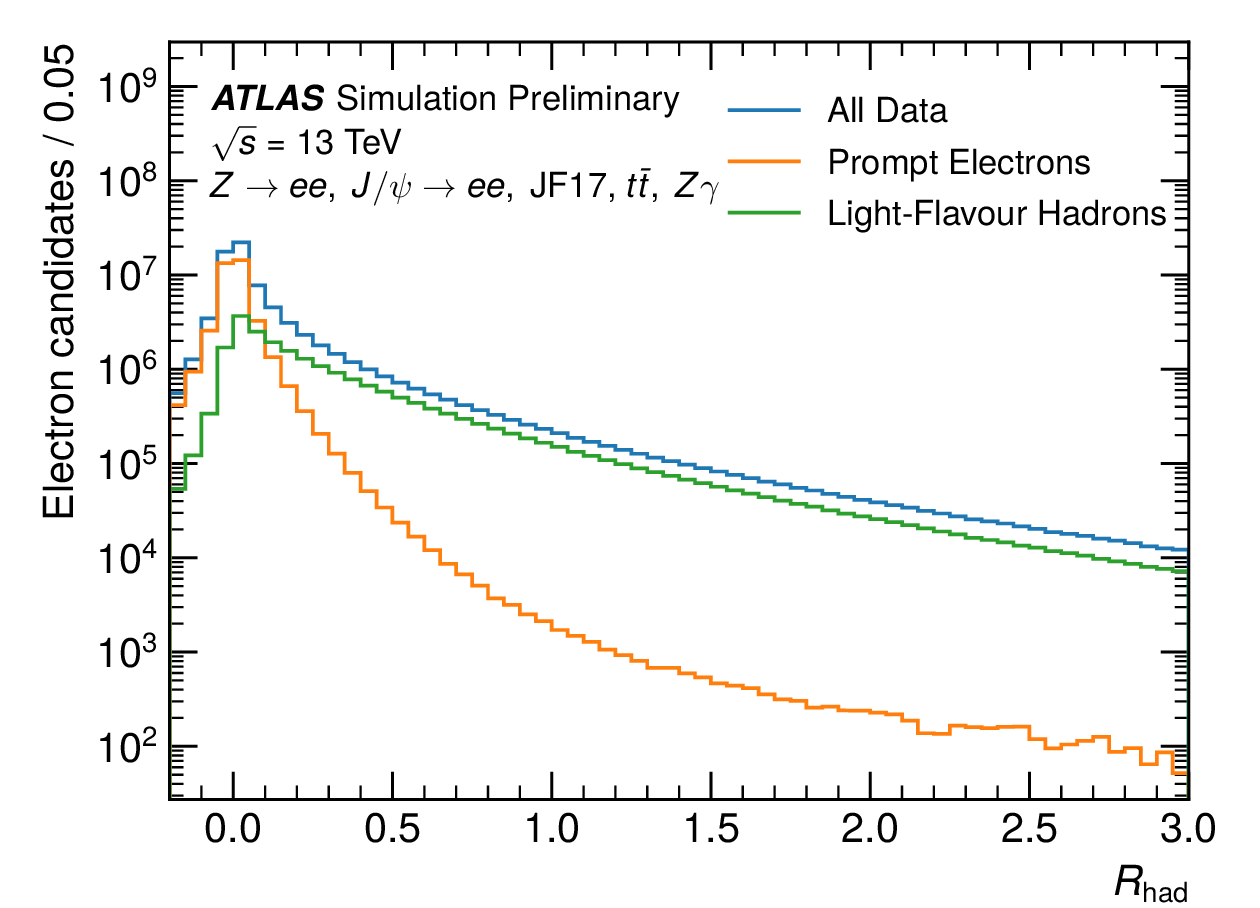
\includegraphics[width=\textwidth]{rhad_original.png}
      \caption{}
  \end{subfigure}
  \hfill
  \begin{subfigure}[b]{0.45\textwidth}
      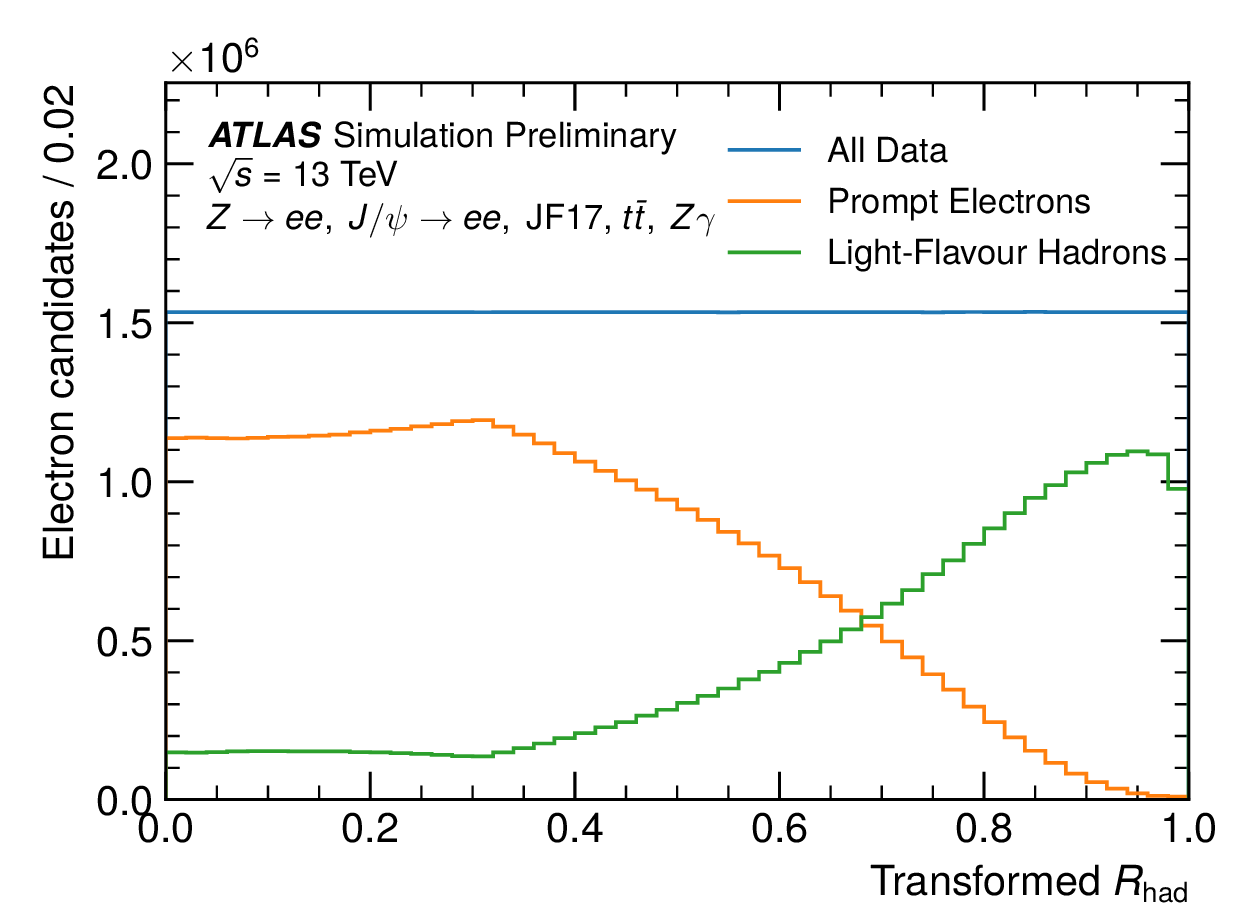
\includegraphics[width=\textwidth]{rhad_transformed.png}
      \caption{}
  \end{subfigure}
  \hfill
  \caption{Distribution of $R_{\text{had}}$ for all candidates, prompt electrons, and Light-Flavour hadrons, shown (a) before and (b) after applying the QuantileTransformer. Distributions include downsampling and reweighting and only two classes are displayed for clarity. In these studies presented in Ref.~\cite{dnn_paper}, an additional $Z\gamma$ input was used.}
  \label{fig:transformed}
\end{figure}

\subsubsection{Training procedure}

In our specific case, it has been employed a Deep Neural Network with a total of five hidden layers, each containing 256 nodes. In these hidden layers, the Leaky ReLU activation function is applied to introduce non-linearity, as detailed in Sec.~\ref{subsec:dnn_general}, and batch normalization is also implemented.  
This algorithm performs a multinomial classification, producing as output a total of six scores, one for prompt electrons and five for each of the background classes. In the final output layer, the Softmax activation function is applied.  
A schematic diagram of our DNN architecture is shown in Figure~\ref{dnn_sketch}.

\begin{figure}[htbp]
  \centering
  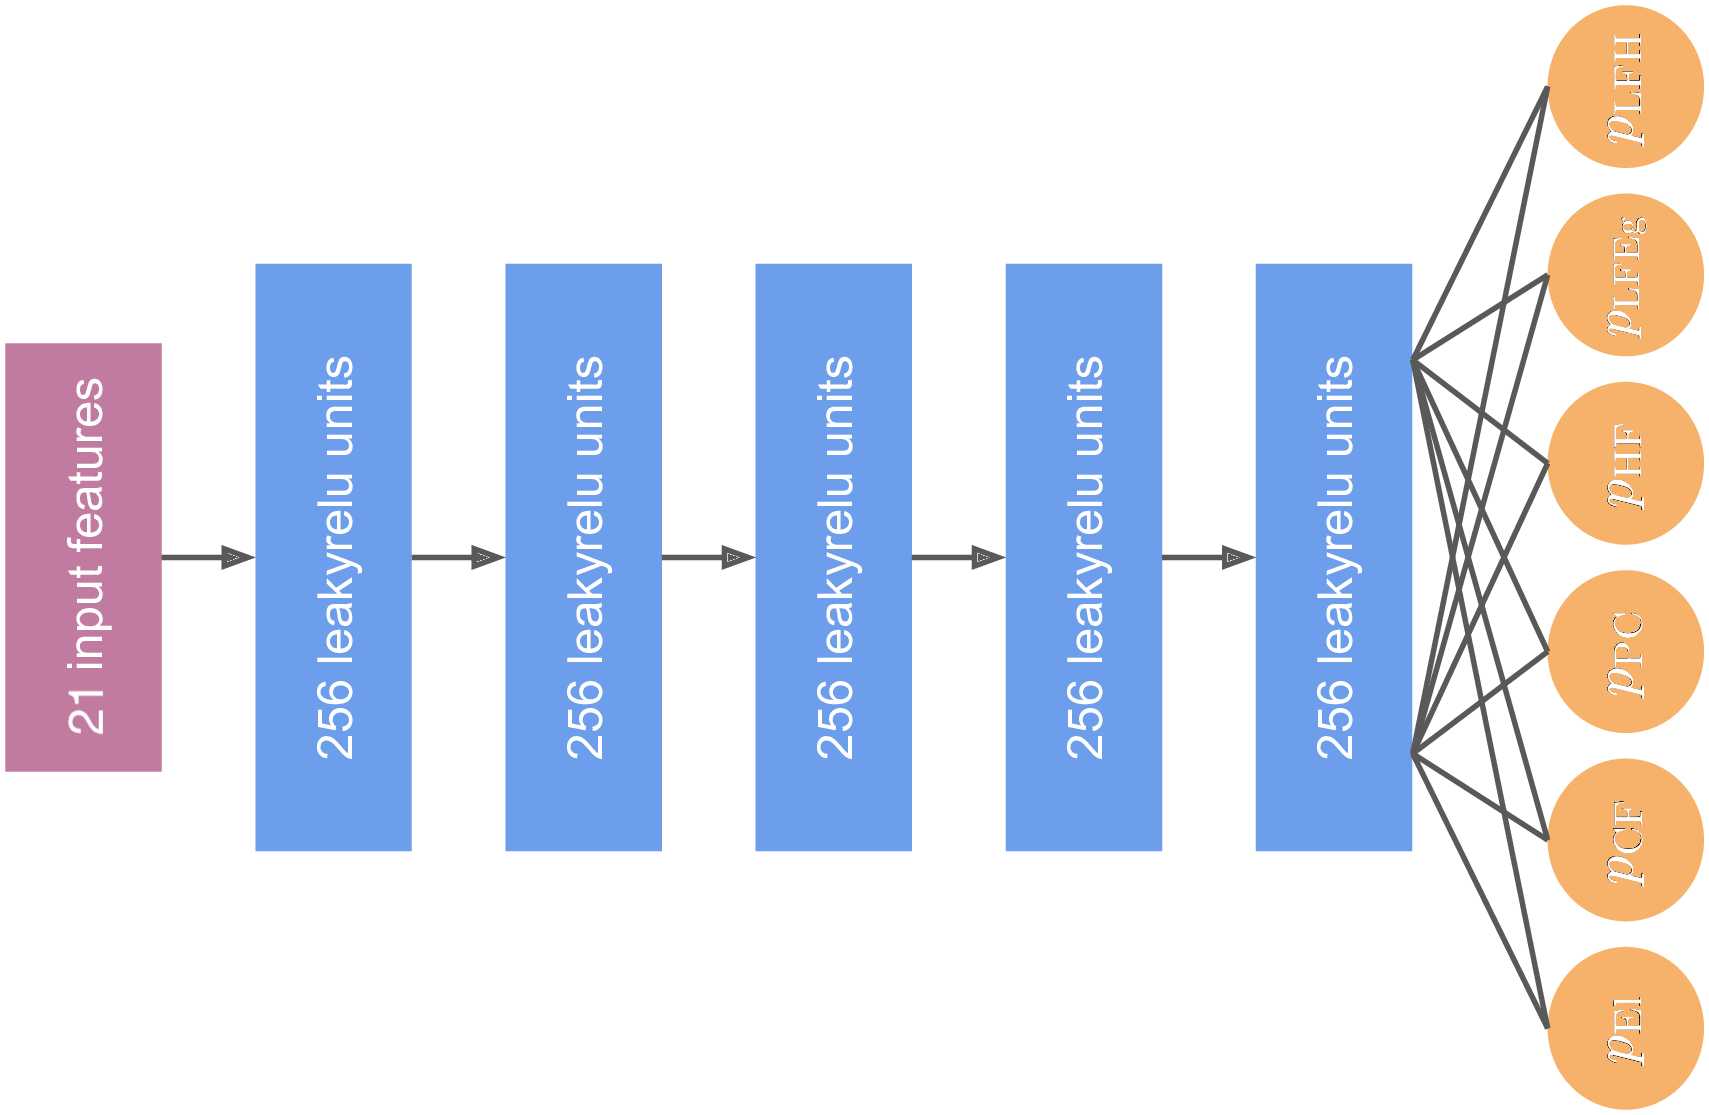
\includegraphics[width=0.8\textwidth]{dnn_sketch.png}
  \caption{Overview diagram of the architecture of the electron identification DNN. It is shown the optimised number of layers and nodes used in the final version. Taken from Ref.~\cite{dnn_paper}.}
  \label{dnn_sketch}
\end{figure}

This algorithm was implemented and trained using the \texttt{Python} \texttt{tensorflow} library~\cite{tensorflow2015}, version~2.4. As previously mentioned, the $Adam$ optimizer was used in the training procedure. Regarding the remaining hyperparameters of the neural network, different configurations were tested, and the one showing the best performance was selected.  
The final training is performed over a total of 100 epochs, retaining as the final result the iteration that yields the lowest loss on the validation dataset.

\subsubsection{Electron classification}

The decision to employ a multinomial classification as the output of our DNN stems from the fact that we distinguish between the different background classes that typically populate our real collision data. There are not only kinematic differences among these classes of electron candidates, but also the chosen input variables are potentially different for each of them. This is due, for example, to the distinct characteristics of the calorimeter showers they produce in the detector. As an illustration, electron candidates originating from $b$- or $c$-hadrons tend to deposit more energy in the innermost layers than prompt electrons, as can be seen in Figure~\ref{fig:input2}.

Nevertheless, for the purpose of identifying signal electrons over the rest of the background candidates, a binomial discrimination must ultimately be performed when defining our working points as a function of efficiencies.  
For this, the following binomial discriminant is defined, simply combining the output given by the DNN:

\begin{equation}
  \small
  %\footnotesize
  \mathcal{D}_{el} = \frac{f_{El}p_{El} + (1-f_{El})p_{CF}}{f_{PC}p_{PC}+f_{HF}p_{HF}+f_{LFEg}p_{LFEg}+(1-f_{PC}-f_{HF}-f_{LFEg})p_{LFH}}
\label{dnn_discriminant}
\end{equation}
where $p_{X}$ are the scores provided by the DNN for each class, and $f_{X}$ are tunable parameters or weights, referred to as \textit{fractions}, which control the relative importance of the different classes in the discriminant.  
This discriminant separates electron candidates considered as signal, in a generic electron identification problem, which in this case are prompt and Charge-Flip electrons (therefore placed in the numerator), from the remaining background electrons in the denominator.

As mentioned, the fractions $f_{X}$ are tunable, and to simplify the procedure it is imposed that their sum equals unity in both numerator and denominator. Depending on the physics analysis under study and the composition of its final states, one background class may be more relevant than another, and this is fully configurable here.

Ideally, the determination of these fractions would be performed directly from real data, just as is done for the LH during training. However, obtaining sufficiently pure and unbiased control regions from data is a highly challenging task, and mixing real data for some classes with MC simulations for others can be risky in a neural network, as the algorithm may directly learn from mismodellings.

For this reason, in our generic electron identification studies, the fractions are tuned and the performance of the DNN is evaluated using the test dataset obtained from the simulated input samples. As previously explained, the test dataset is a fraction of the initial dataset unseen by the neural network during training, containing electron candidates from all predefined classes and originating from the four physics processes initially presented. This ensures a representative collection of candidates covering the full energy spectrum and all detector regions, which will resemble as closely as possible what will later be encountered in real data.

Moreover, since it would not be meaningful to apply any reweighting or downsampling here, as is done for the training and validation datasets, the tuning of the fractions, the evaluation of the algorithm’s performance, and the subsequent derivation of working points are performed in bins of $|\eta|$ and/or $E_{\text{T}}$.  
As a figure of merit for estimating the performance of our algorithm and comparing it to the LH, we use ROC curves, already described in Sec.~\ref{sec:ml_methods}. Before constructing the discriminant, we must first determine the fractions to be used.

The calculation of the $f_{X}$ is performed in different $|\eta|$ bins to account for variations in the spectra of the different electron candidate classes. The same fractions are applied across the full $E_{\text{T}}$ range to obtain a smooth and continuous discriminant over the entire energy spectrum.

The optimal $f_{X}$ values are determined by maximising the Area Under the Curve (AUC) of the ROC between $70\%$ and $95\%$ signal efficiency, which essentially covers the typical range used in most working points for electron identification. The $|\eta|$ bins employed here are broader than those used later when defining the DNN working points, which apply cuts on the discriminant as explained in Sec.~\ref{dnn:tuning}.  
Table~\ref{tune:binning} lists the $|\eta|$ and $E_{\text{T}}$ bin boundaries used in each case.

\begin{table}[htbp]
  \centering
  \caption{Bin edges used for the discriminant cuts and for the $f_X$ optimisation.}
  \footnotesize
  \setlength{\tabcolsep}{5pt}
  \renewcommand{\arraystretch}{1.1}

  % Primera tabla: |eta|
  \begin{subtable}[t]{\linewidth}
    \centering
    \subcaption{Bin boundaries in $|\eta|$}
    \vspace{2pt}
    \begin{tabular}{@{}ll@{}}
      \toprule
      \textbf{Use} & \textbf{Edges} \\
      \midrule
      Discriminant cuts &
      $0.0,\ 0.1,\ 0.6,\ 0.8,\ 1.15,\ 1.37,\ 1.52,\ 1.81,\ 2.01,\ 2.37,\ 2.47$ \\
      $f_X$ optimisation &
      $0.0,\ 0.8,\ 1.37,\ 1.52,\ 2.01,\ 2.47$ \\
      \bottomrule
    \end{tabular}
  \end{subtable}

  \vspace{0.4cm} % separación entre tablas

  % Segunda tabla: ET
  \begin{subtable}[t]{\linewidth}
    \centering
    \subcaption{Bin boundaries in $E_{\text{T}}$ [GeV]}
    \vspace{2pt}
    \begin{tabular}{@{}ll@{}}
      \toprule
      \textbf{Use} & \textbf{Edges} \\
      \midrule
      Discriminant cuts &
      $4,\ 7,\ 10,\ 15,\ 20,\ 25,\ 30,\ 35,\ 40,\ 45,\ \infty$ \\
      \bottomrule
    \end{tabular}
  \end{subtable}
  \label{tune:binning}
\end{table}

As mentioned, the $f_{X}$ values obtained in these bins from our test sample are optimal for our studies. However, in other analyses the dataset composition will very likely differ, and these values can therefore be adjusted accordingly.  

With the $ \mathcal{D}_{el} $ discriminant now defined, Figure~\ref{fig:dnn_final_disc} shows its distribution evaluated for the different electron candidate classes, for a specific $|\eta|$ and $E_{\text{T}}$ bin.
\begin{figure}[htbp]
  \centering
  % Fila superior: (a) y (b)
  \begin{subfigure}[t]{0.48\linewidth}
    \centering
    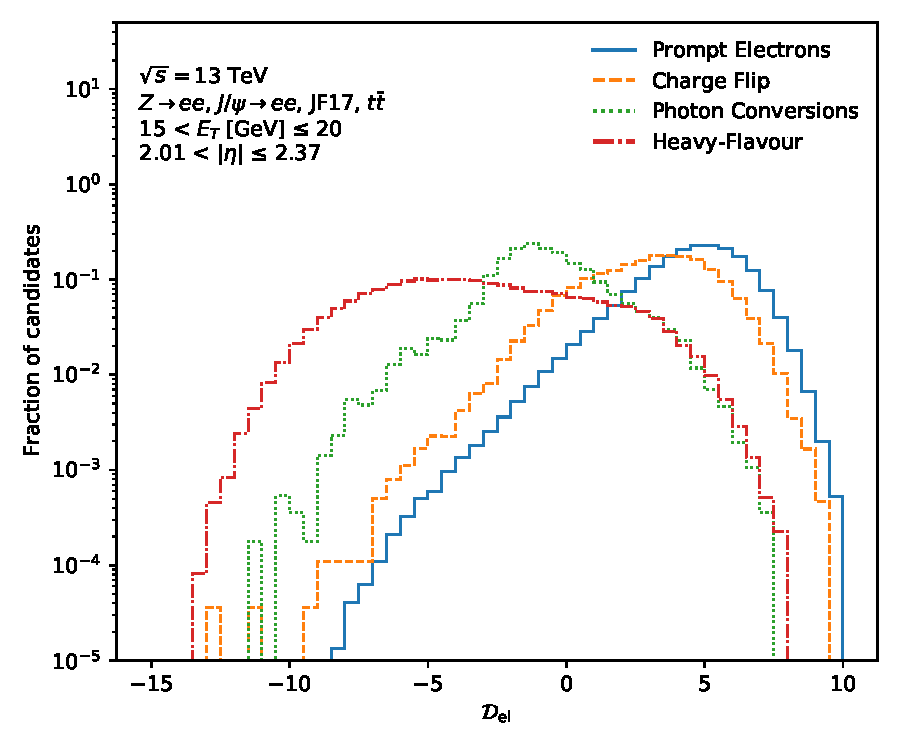
\includegraphics[width=\linewidth]{discriminant_plots/panel_a.pdf}
    \caption{}
    \label{fig:dnnDisc_a}
  \end{subfigure}\hfill
  \begin{subfigure}[t]{0.48\linewidth}
    \centering
    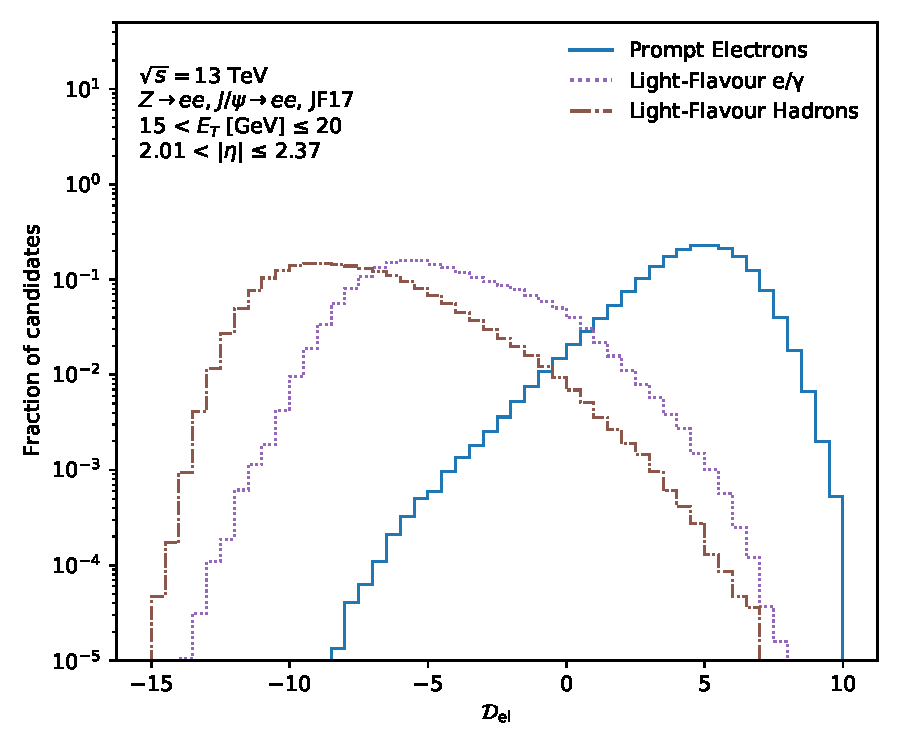
\includegraphics[width=\linewidth]{discriminant_plots/panel_b.pdf}
    \caption{}
    \label{fig:dnnDisc_b}
  \end{subfigure}

  \vspace{0.35cm}

  % Fila inferior: (c)
  \begin{subfigure}[t]{0.60\linewidth}
    \centering
    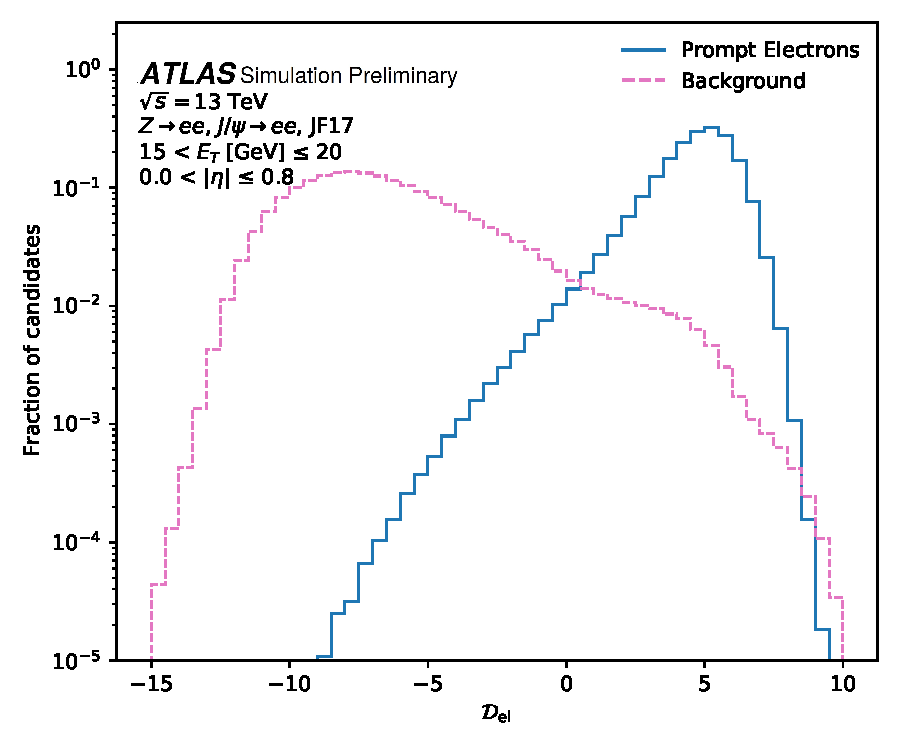
\includegraphics[width=\linewidth]{discriminant_plots/panel_c.pdf}
    \caption{}
    \label{fig:dnnDisc_c}
  \end{subfigure}

  \caption{Signal discriminant $D_{\mathrm{el}}$ of the DNN shown for (a) prompt electrons,
  Charge-Flip electrons, photon conversions, and electrons from Heavy-Flavour decays;
  (b) prompt electrons, $e/\gamma$ objects from Light-Flavour decays, and Light-Flavour hadrons;
  and (c) prompt electrons versus the combined background (all classes except prompt and Charge-Flip).
  Candidates satisfy $15<E_{T}\leq 20~\mathrm{GeV}$ and $0.0<|\eta|\leq 0.8$.}
  \label{fig:dnn_final_disc}
\end{figure}
The relative contribution of each background electron class in the test sample used can be found in Table~\ref{tab:relative_contribution}, both inclusively and for the specific kinematic bin under study $(E_{\text{T}},|\eta|)$.

\begin{table}[htbp]
  \centering
  \begingroup
  \scriptsize
  \setlength{\tabcolsep}{3pt}
  \renewcommand{\arraystretch}{1.05}
  \begin{subtable}[t]{0.49\linewidth}
    \centering
    \subcaption{Inclusive}
    \vspace{2pt}
    \begin{tabularx}{\linewidth}{{\raggedright\arraybackslash}{}}
      \toprule
      \textbf{Class} & \textbf{Fraction [\%]} & \textbf{Stat. error} \\
      \midrule
      Photon Conversions      & 0.3251  & $\pm$ 0.0010 \\
      Heavy-Flavour           & 7.444  & $\pm$ 0.002 \\
      Light-Flavour e/$\gamma$& 17.731 & $\pm$ 0.003 \\
      Light-Flavour Hadrons   & 71.796 & $\pm$ 0.007 \\
      \bottomrule
    \end{tabularx}
  \end{subtable}\hfill
  \begin{subtable}[t]{0.49\linewidth}
    \centering
    \subcaption{\scriptsize{$15<E_{T}\leq 20~\mathrm{GeV}$, $0.0<|\eta|\leq 0.8$}}
    \vspace{2pt}
    \begin{tabularx}{\linewidth}{{\raggedright\arraybackslash}{}}
      \toprule
      \textbf{Class} & \textbf{Fraction [\%]} & \textbf{Stat. error} \\
      \midrule
      Photon Conversions      & 0.611  & $\pm$ 0.004 \\
      Heavy-Flavour           & 19.658 & $\pm$ 0.024 \\
      Light-Flavour e/$\gamma$& 11.9460 & $\pm$ 0.019 \\
      Light-Flavour Hadrons   & 66.630 & $\pm$ 0.045 \\
      \bottomrule
    \end{tabularx}
  \end{subtable}
  \endgroup
  \caption{Fractions and statistical errors for all candidates and for the selected kinematic bin.}
  \label{tab:relative_contribution}
\end{table}

In Figure~\ref{fig:dnn_final_disc}, it can be observed that both signal electron classes, prompt and Charge-Flip, reach higher discriminant values, showing a more or less pronounced peak compared to the other background classes. Prompt electrons present a more distinctive distribution than Charge-Flip electrons, although in both cases there is a considerable population of Heavy-Flavour and Photon-Conversion background candidates toward the higher end of the range. However, these background distributions also tend to peak at lower discriminant values, which is equally important for achieving high identification efficiencies when defining thresholds.

It is worth noting that Heavy-Flavour electrons tend to populate a wide range of discriminant values compared to signal electrons, and in some cases even overlap with Photon-Conversion electrons. This can be explained by the fact that they originate from the decay of heavy quarks (b- and c-hadrons). If these hadrons had a shorter lifetime, their signatures and detector energy deposits would be more similar to those of prompt electrons, or even electrons from converted photons, which themselves can also be prompt. Part of this overlap is in fact reduced by the application of the rectangular cuts discussed previously.

In contrast, as seen in Figure~\ref{fig:dnnDisc_b}, the distributions of the Light-Flavour classes differ clearly from those of prompt electrons, which is highly advantageous and demonstrates the potential of our algorithm to reject these classes.

\subsubsection{Identification Performance}

As mentioned earlier, our performance evaluation is based on the ROC curves of the DNN model.
Figure~\ref{fig:roc_mainbkg} shows the ROC curves for prompt electrons against the combined background and each background class individually. The signal definition always includes only prompt electrons, while the LH working points (Loose, Medium, Tight) are represented by single points, located at progressively lower signal efficiencies: Loose around $\varepsilon_{\rm sig} = 0.85$, Medium around $0.75$, and Tight around $0.65$.

Unlike the LH, the DNN curves shown here do not include the additional rectangular cuts listed in Table~\ref{tab:wp_rectangular_cuts}, and therefore correspond to a slightly more relaxed selection. The only requirements applied to the DNN candidates are the minimum numbers of silicon detector hits and pixel hits (7 and 1, respectively), which are the same conditions used to define the training, validation, and testing datasets.

Quantitatively, at the LH~Loose WP, the DNN achieves a background rejection about $2$ times higher than LH when considering all background classes combined. For Heavy-Flavour decays, the improvement at this efficiency is more evident, with a factor close to $2.2$, whereas for Light-Flavour $e/\gamma$ and undecayed hadrons the rejection also increases, by factors of about $4$ and $5$, respectively. Photon conversions show a moderate enhancement, with the DNN reaching a rejection about $2$ times larger than LH. For Charge-Flip electrons, the improvement is striking, with the DNN achieving a rejection almost $8$ times higher than LH in this $\eta$ region.

Figure~\ref{fig:roc_cf} includes the ROC curve calculated for the rejection of Charge-Flip versus prompt electrons, shown here merely to illustrate the capability of the DNN to separate both signal electron classes. In this case, a modified discriminant is used, where the Charge-Flip term is moved to the denominator. In any case, it is important to note that, since the number of prompt electrons largely exceeds that of Charge-Flip electrons in any realistic selection, including Charge-Flip candidates within the signal definition would have a negligible impact on the overall signal efficiency.

The overall improvement of the DNN is clearly visible, with the most notable gains obtained for Light-Flavour hadrons, Light-Flavour $e/\gamma$, and Charge-Flip electrons, the latter benefiting greatly from the new variables added to the DNN, providing a significantly enhanced rejection across the full efficiency range. For Heavy-Flavour electrons, the smaller improvement reflects their closer resemblance to prompt electrons. Photon conversions also benefit moderately from the DNN, as their rejection is already relatively high with LH.

In summary, the DNN consistently outperforms the LH in all background categories, with the most substantial benefits in rejecting backgrounds that exhibit distinctive calorimeter and tracking signatures, and smaller but still relevant gains for more signal-like sources such as Heavy-Flavour decays.

% --- Primera figura ---
\begin{figure}[htbp]
  \centering
  
  \begin{subfigure}[t]{0.6\linewidth}
    \centering
    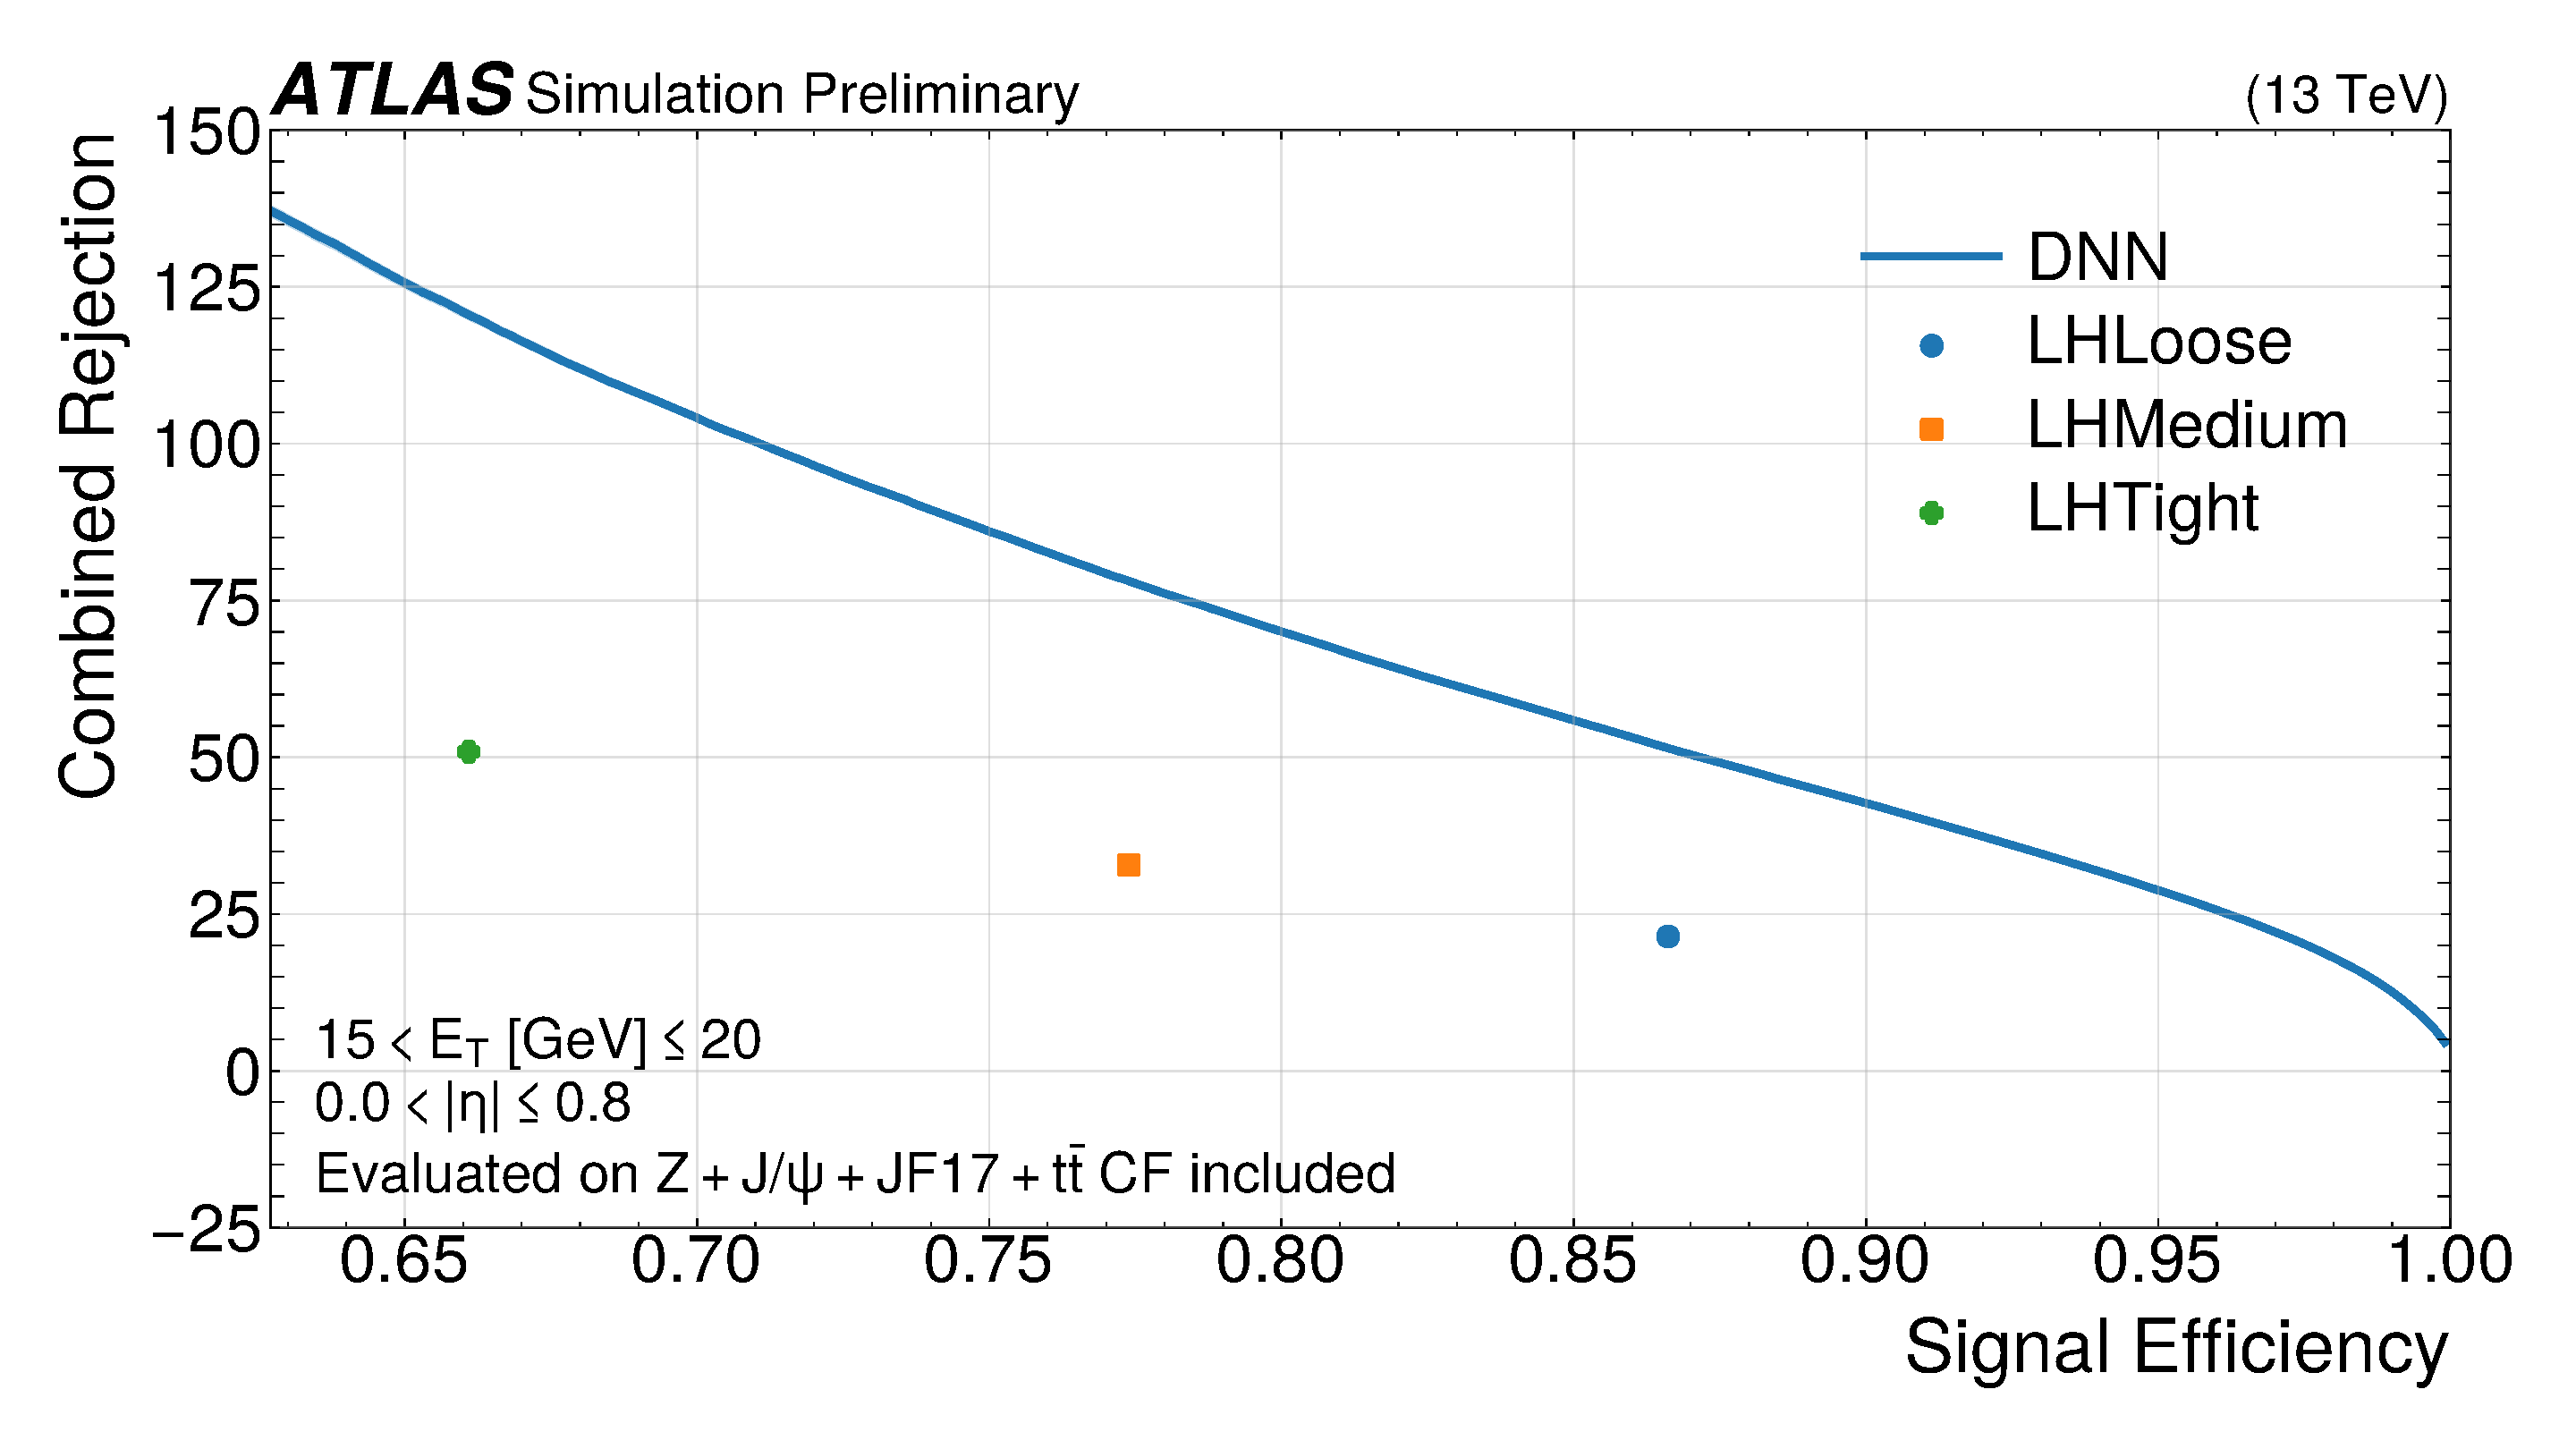
\includegraphics[width=\linewidth]{ROC/15_20_0p0_0p8/binnedROCCurve_et15_20_eta0.0_0.8.pdf}
    \caption{}
    \label{fig:roc_allblkg}
  \end{subfigure}

  \vspace{0.35cm}

  % ---- Fila 1 ----
  \begin{subfigure}[t]{0.5\linewidth}
    \centering
    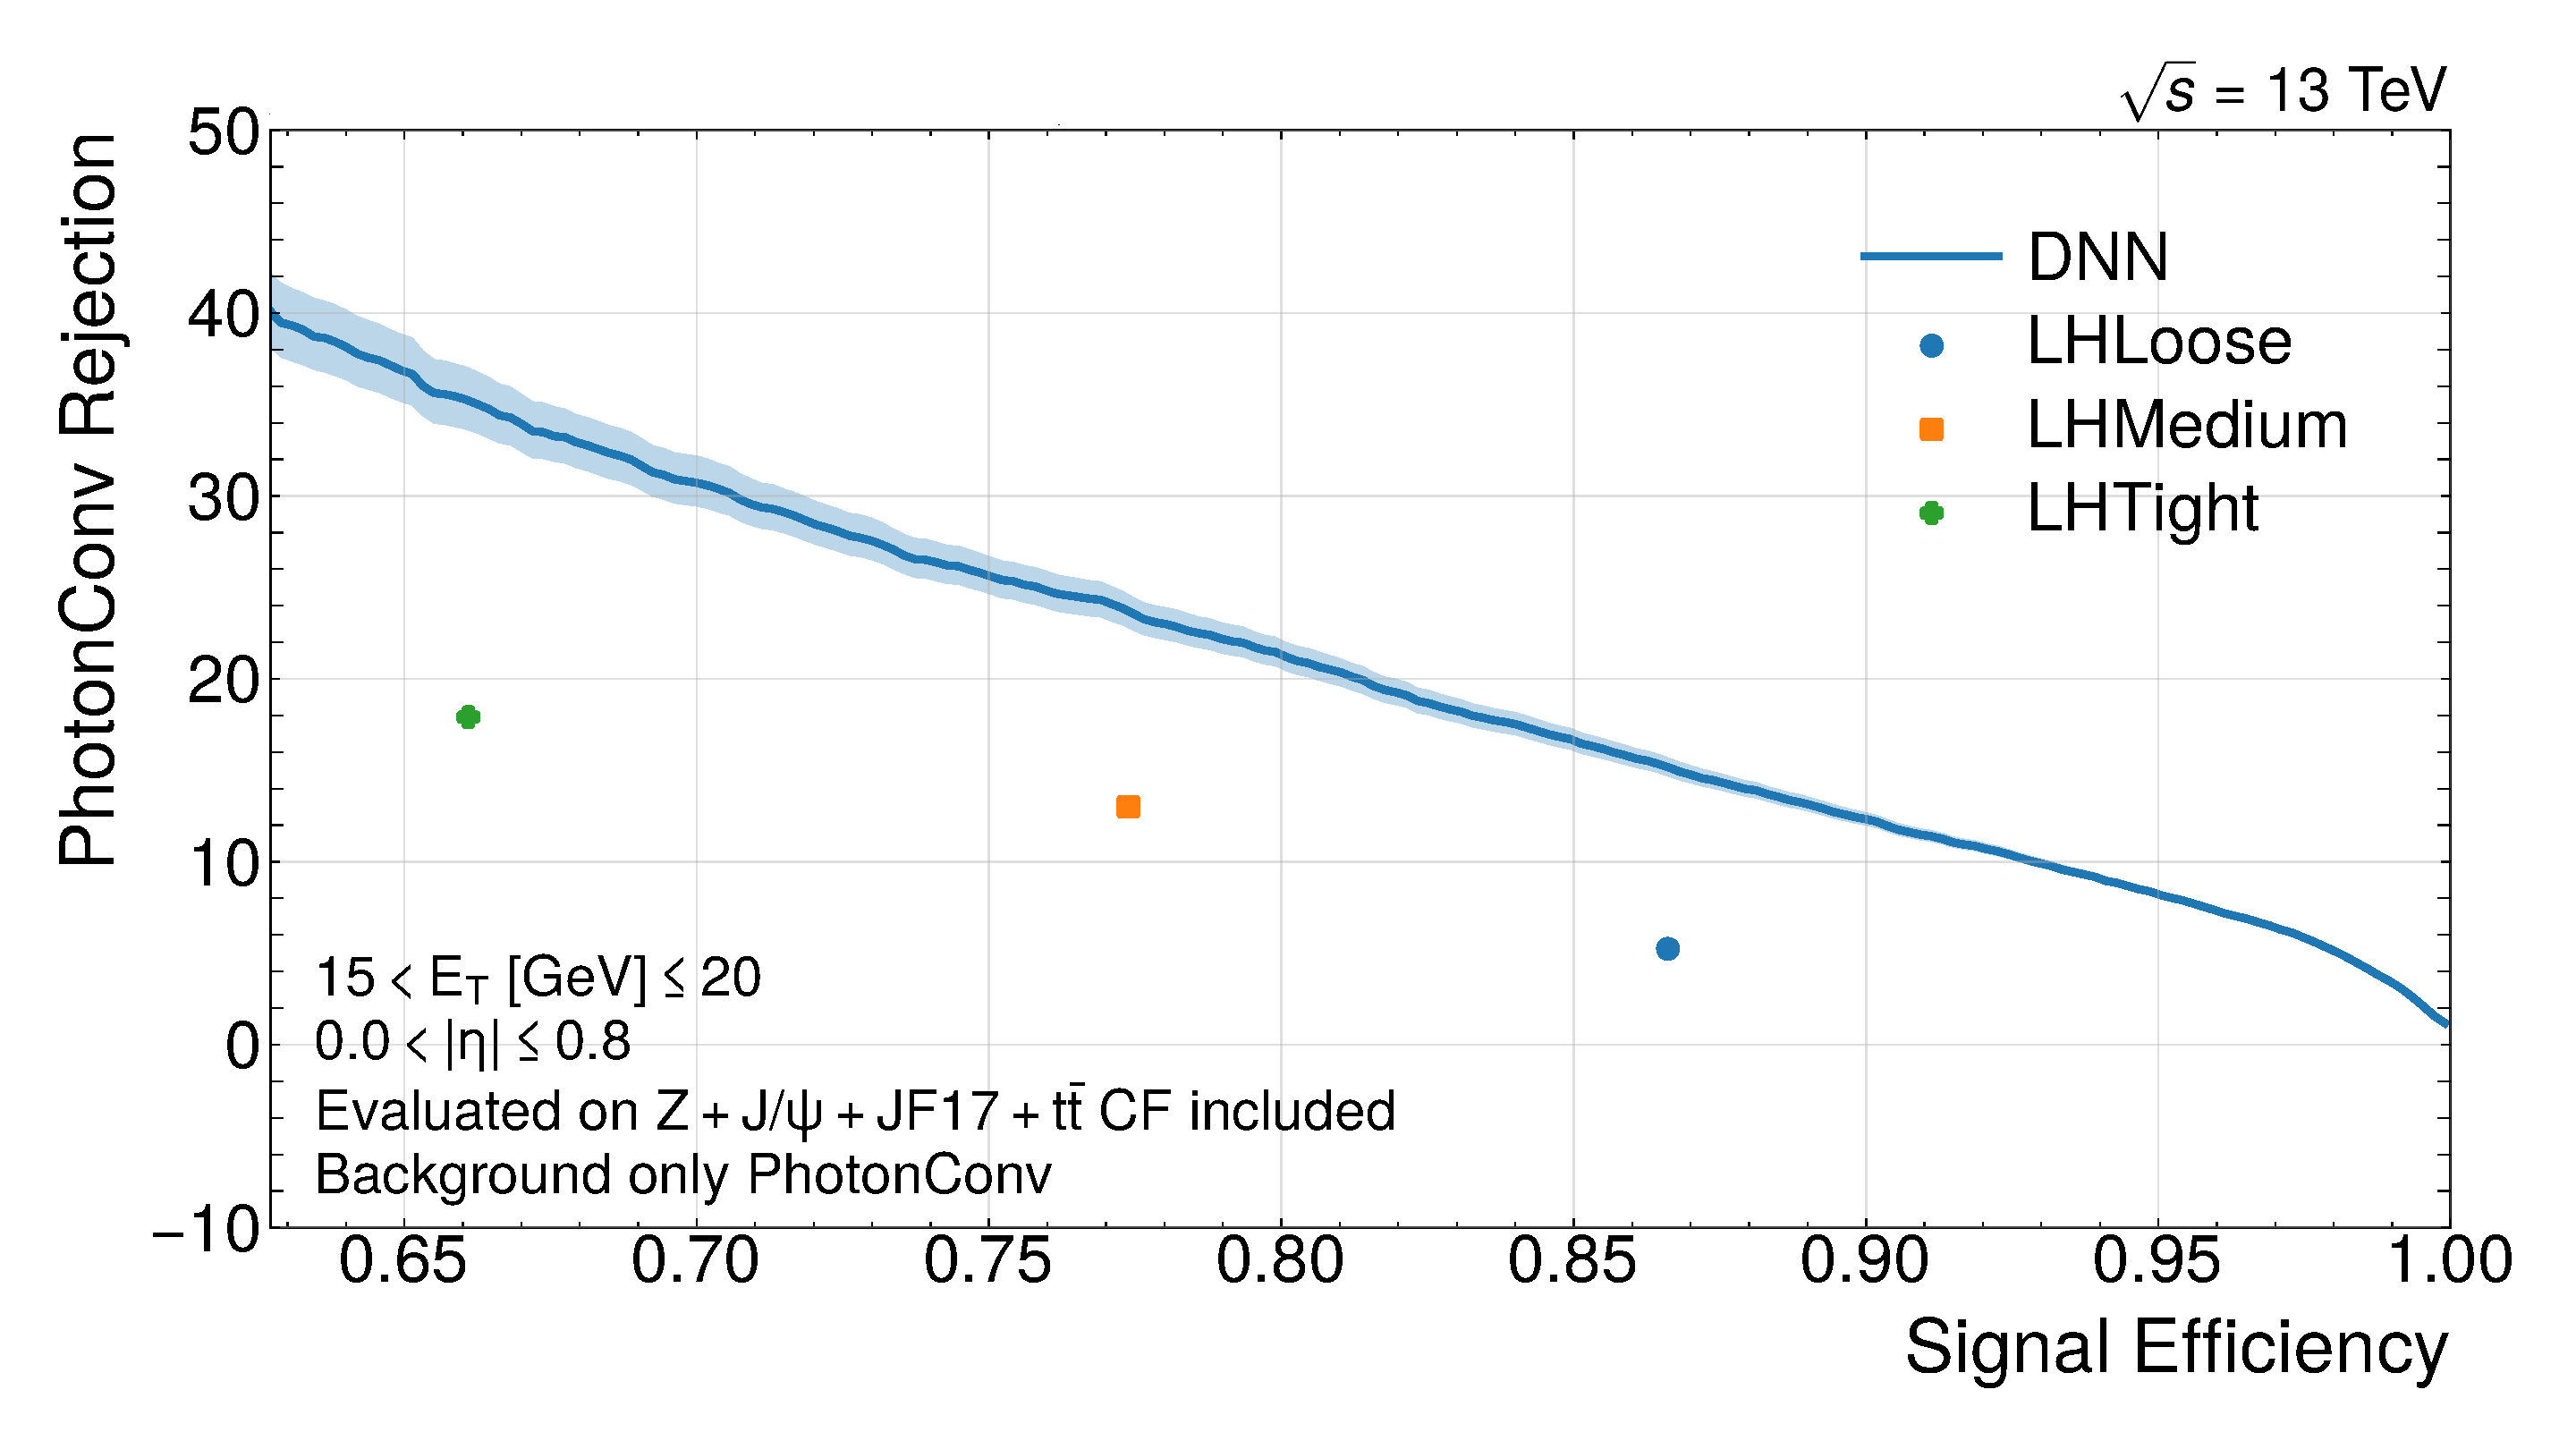
\includegraphics[width=\linewidth]{ROC/15_20_0p0_0p8/binnedROCCurvePhotonConv_et15_20_eta0.0_0.8.pdf}
    \caption{}
    \label{fig:roc_pc}
  \end{subfigure}\hfill
  \begin{subfigure}[t]{0.5\linewidth}
    \centering
    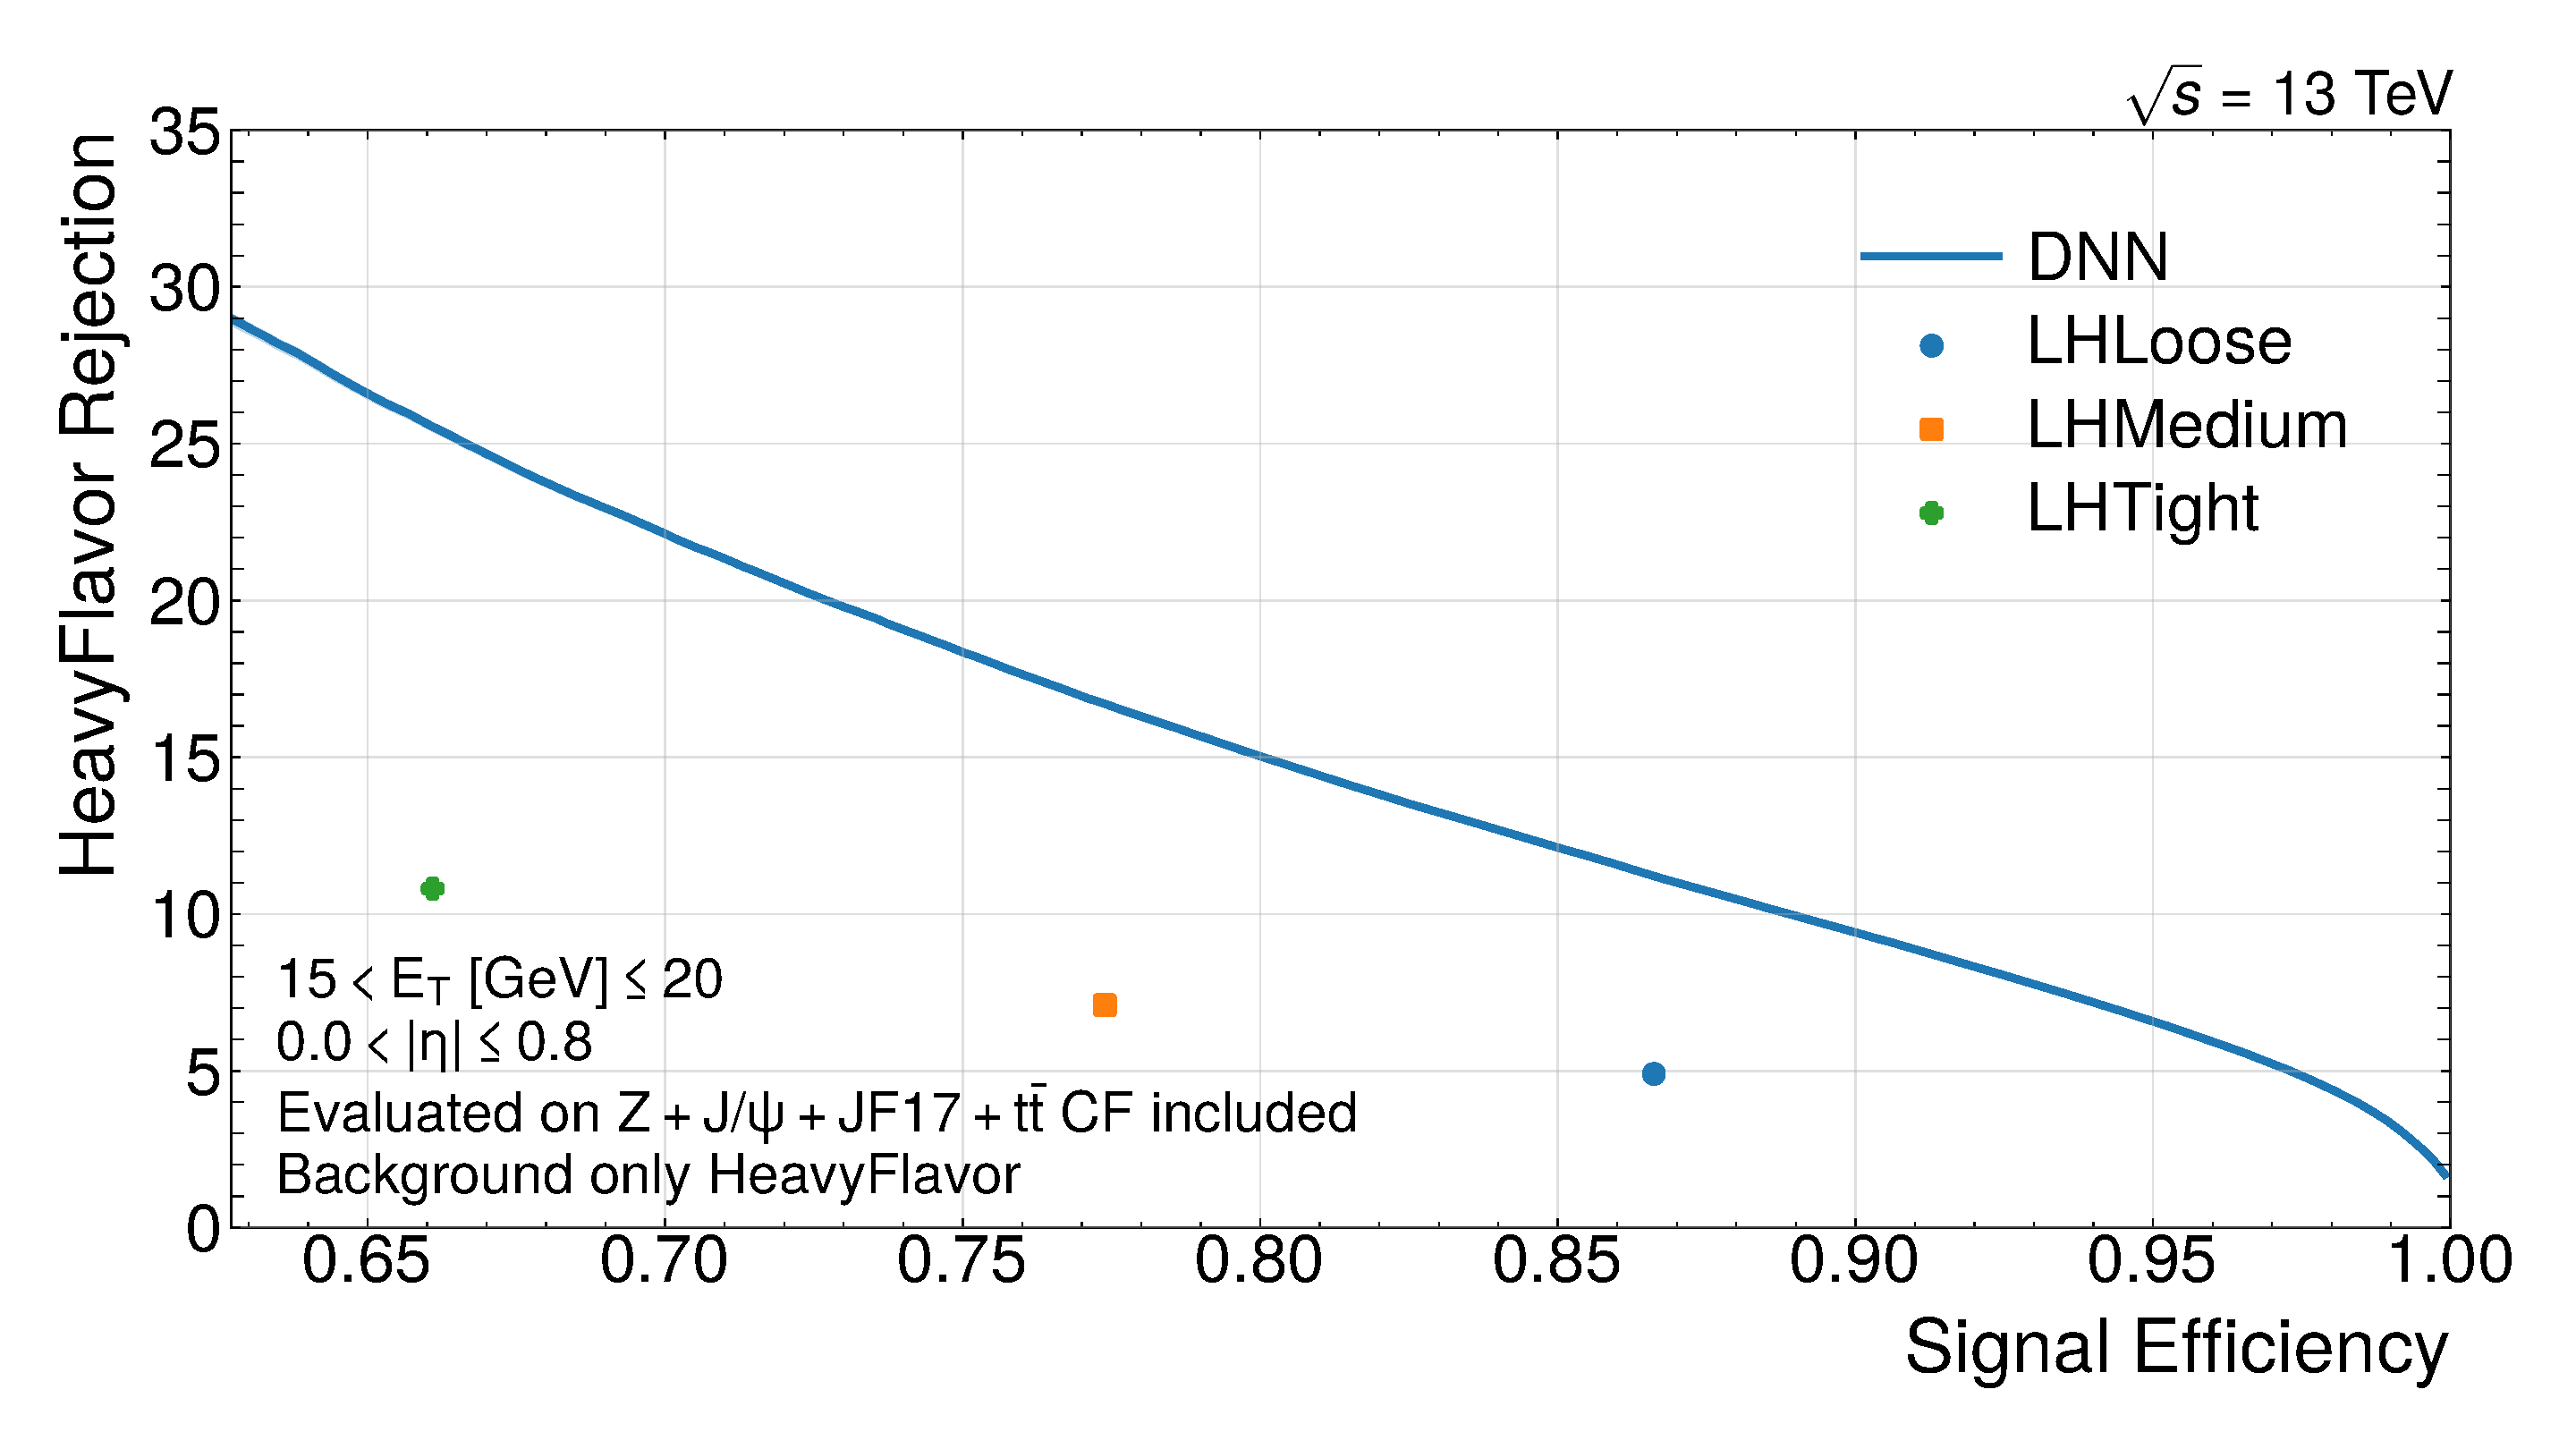
\includegraphics[width=\linewidth]{ROC/15_20_0p0_0p8/binnedROCCurveHeavyFlavor_et15_20_eta0.0_0.8.pdf}
    \caption{}
    \label{fig:roc_hf}
  \end{subfigure}

  \vspace{0.35cm}

  % ---- Fila 2 ----
  \begin{subfigure}[t]{0.5\linewidth}
    \centering
    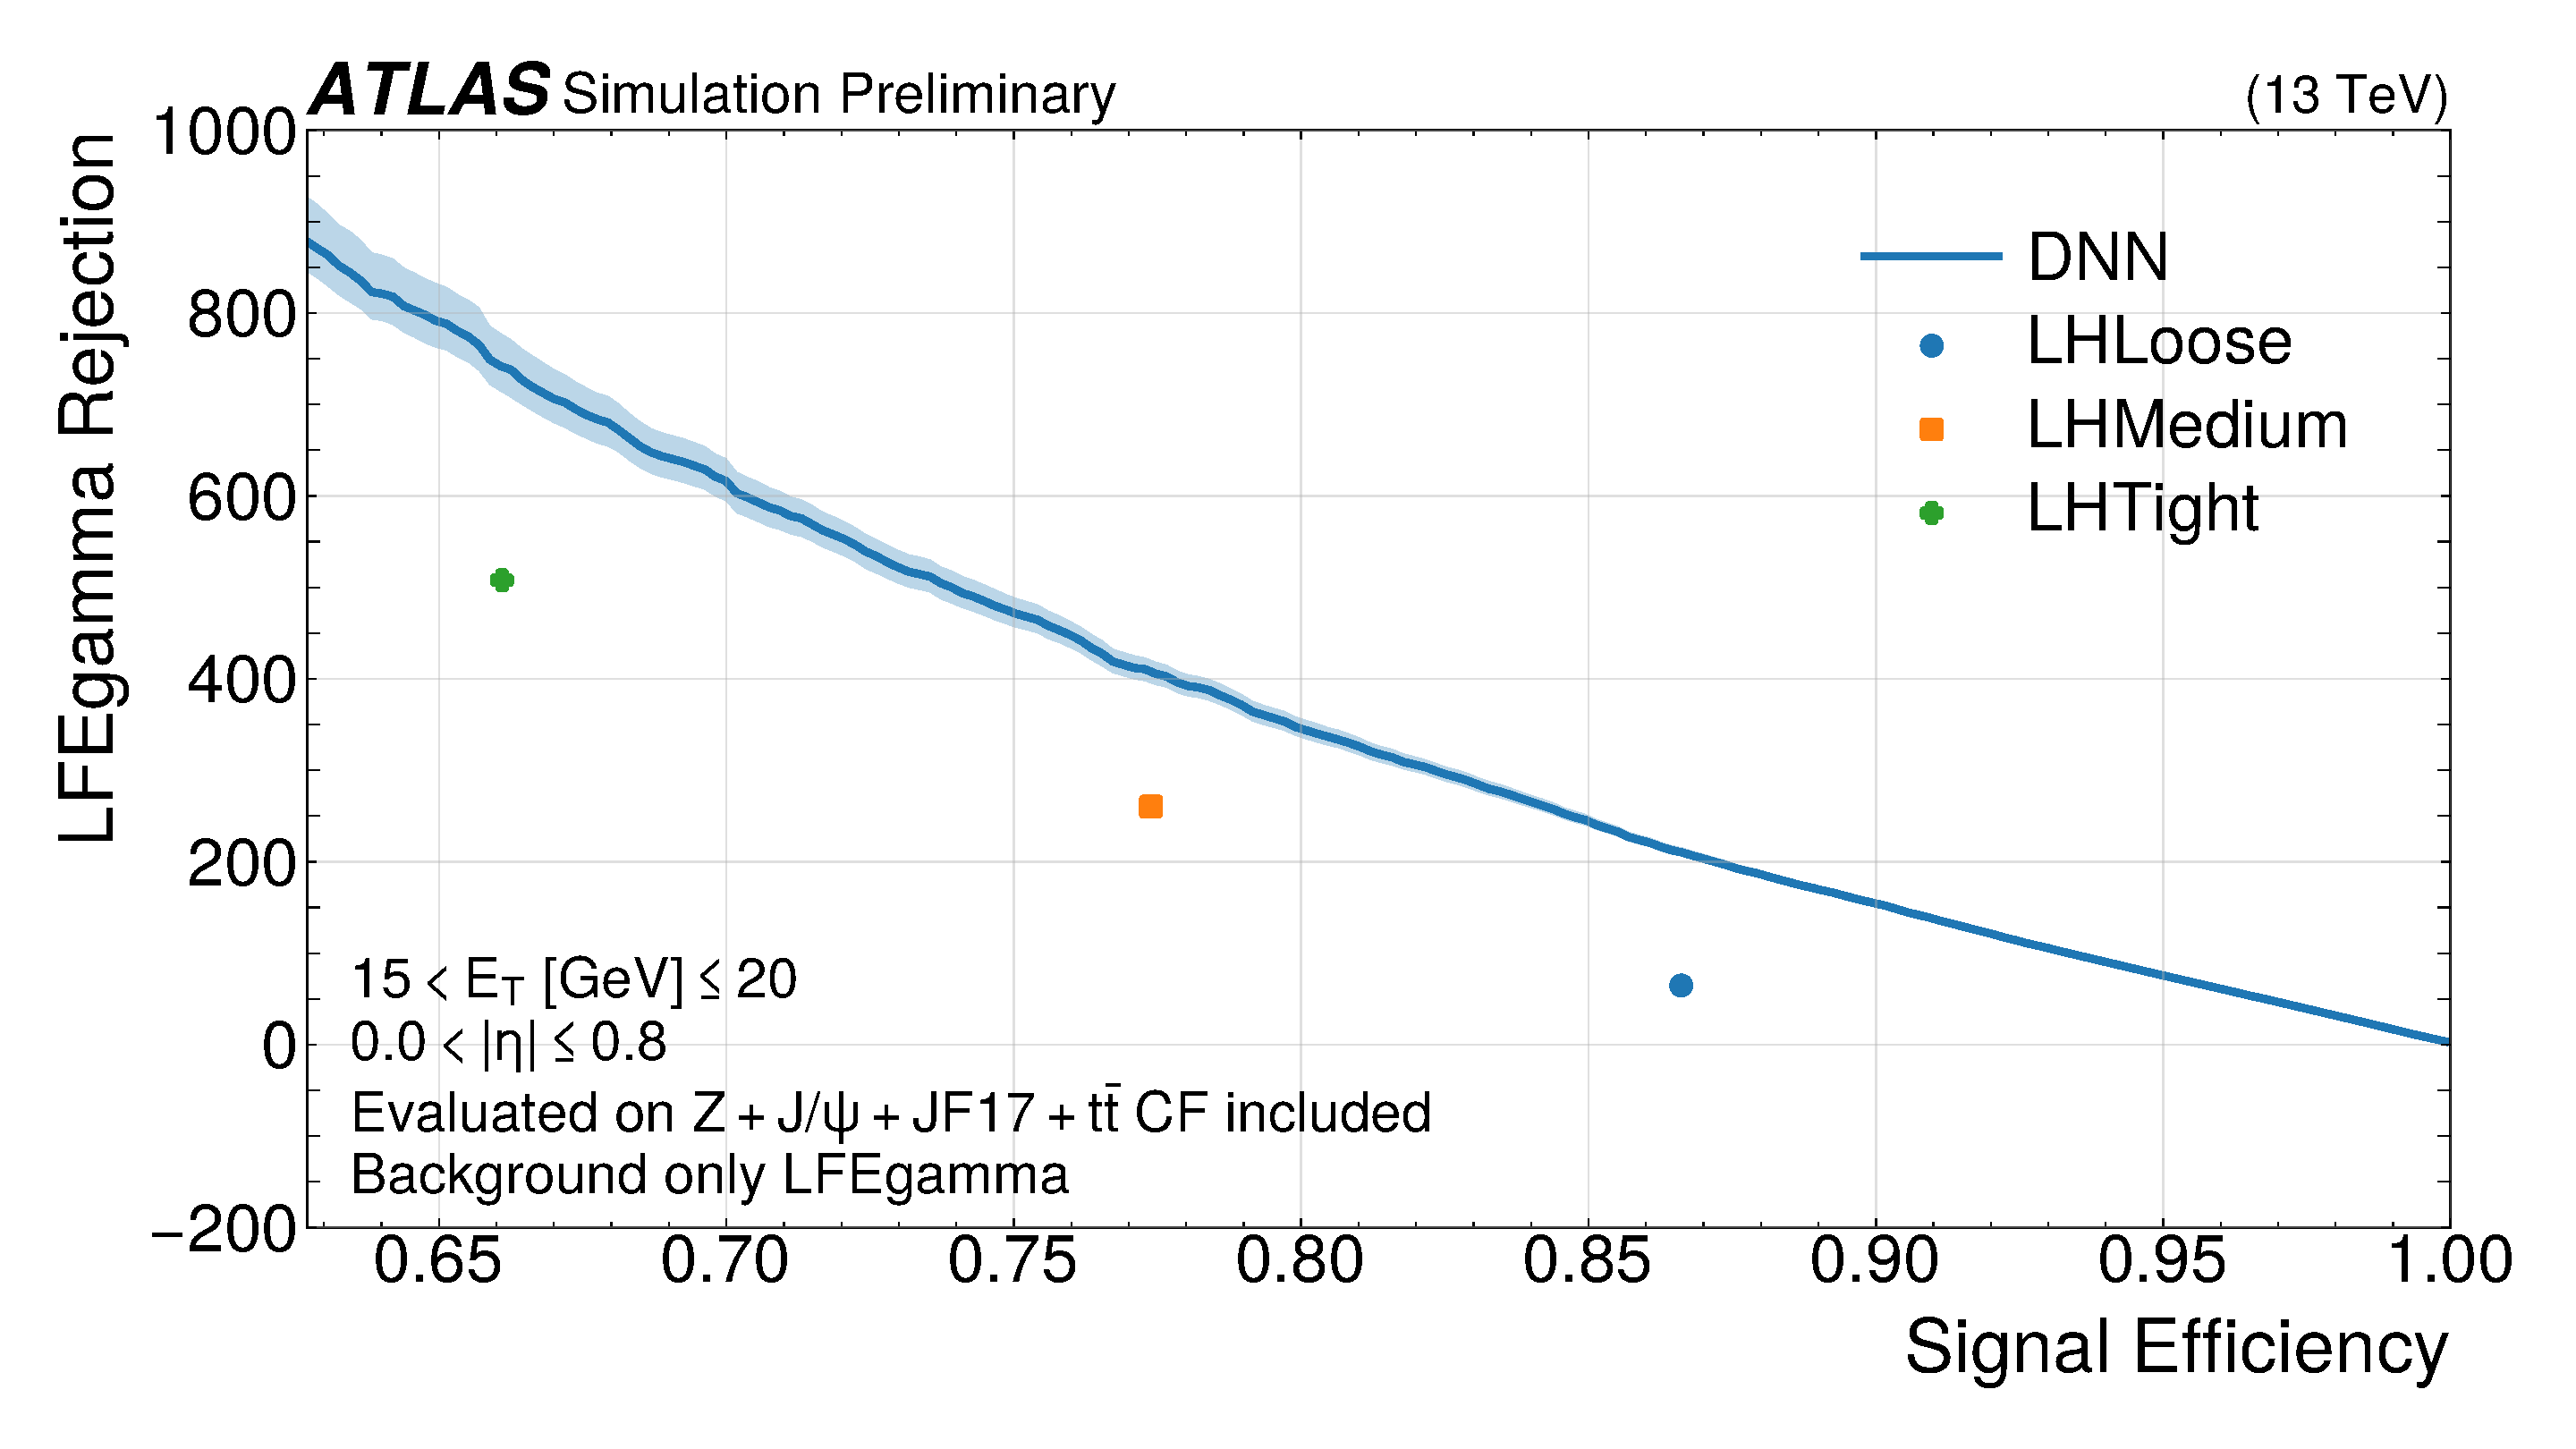
\includegraphics[width=\linewidth]{ROC/15_20_0p0_0p8/binnedROCCurveLFEgamma_et15_20_eta0.0_0.8.pdf}
    \caption{}
    \label{fig:roc_lfeg}
  \end{subfigure}\hfill
  \begin{subfigure}[t]{0.5\linewidth}
    \centering
    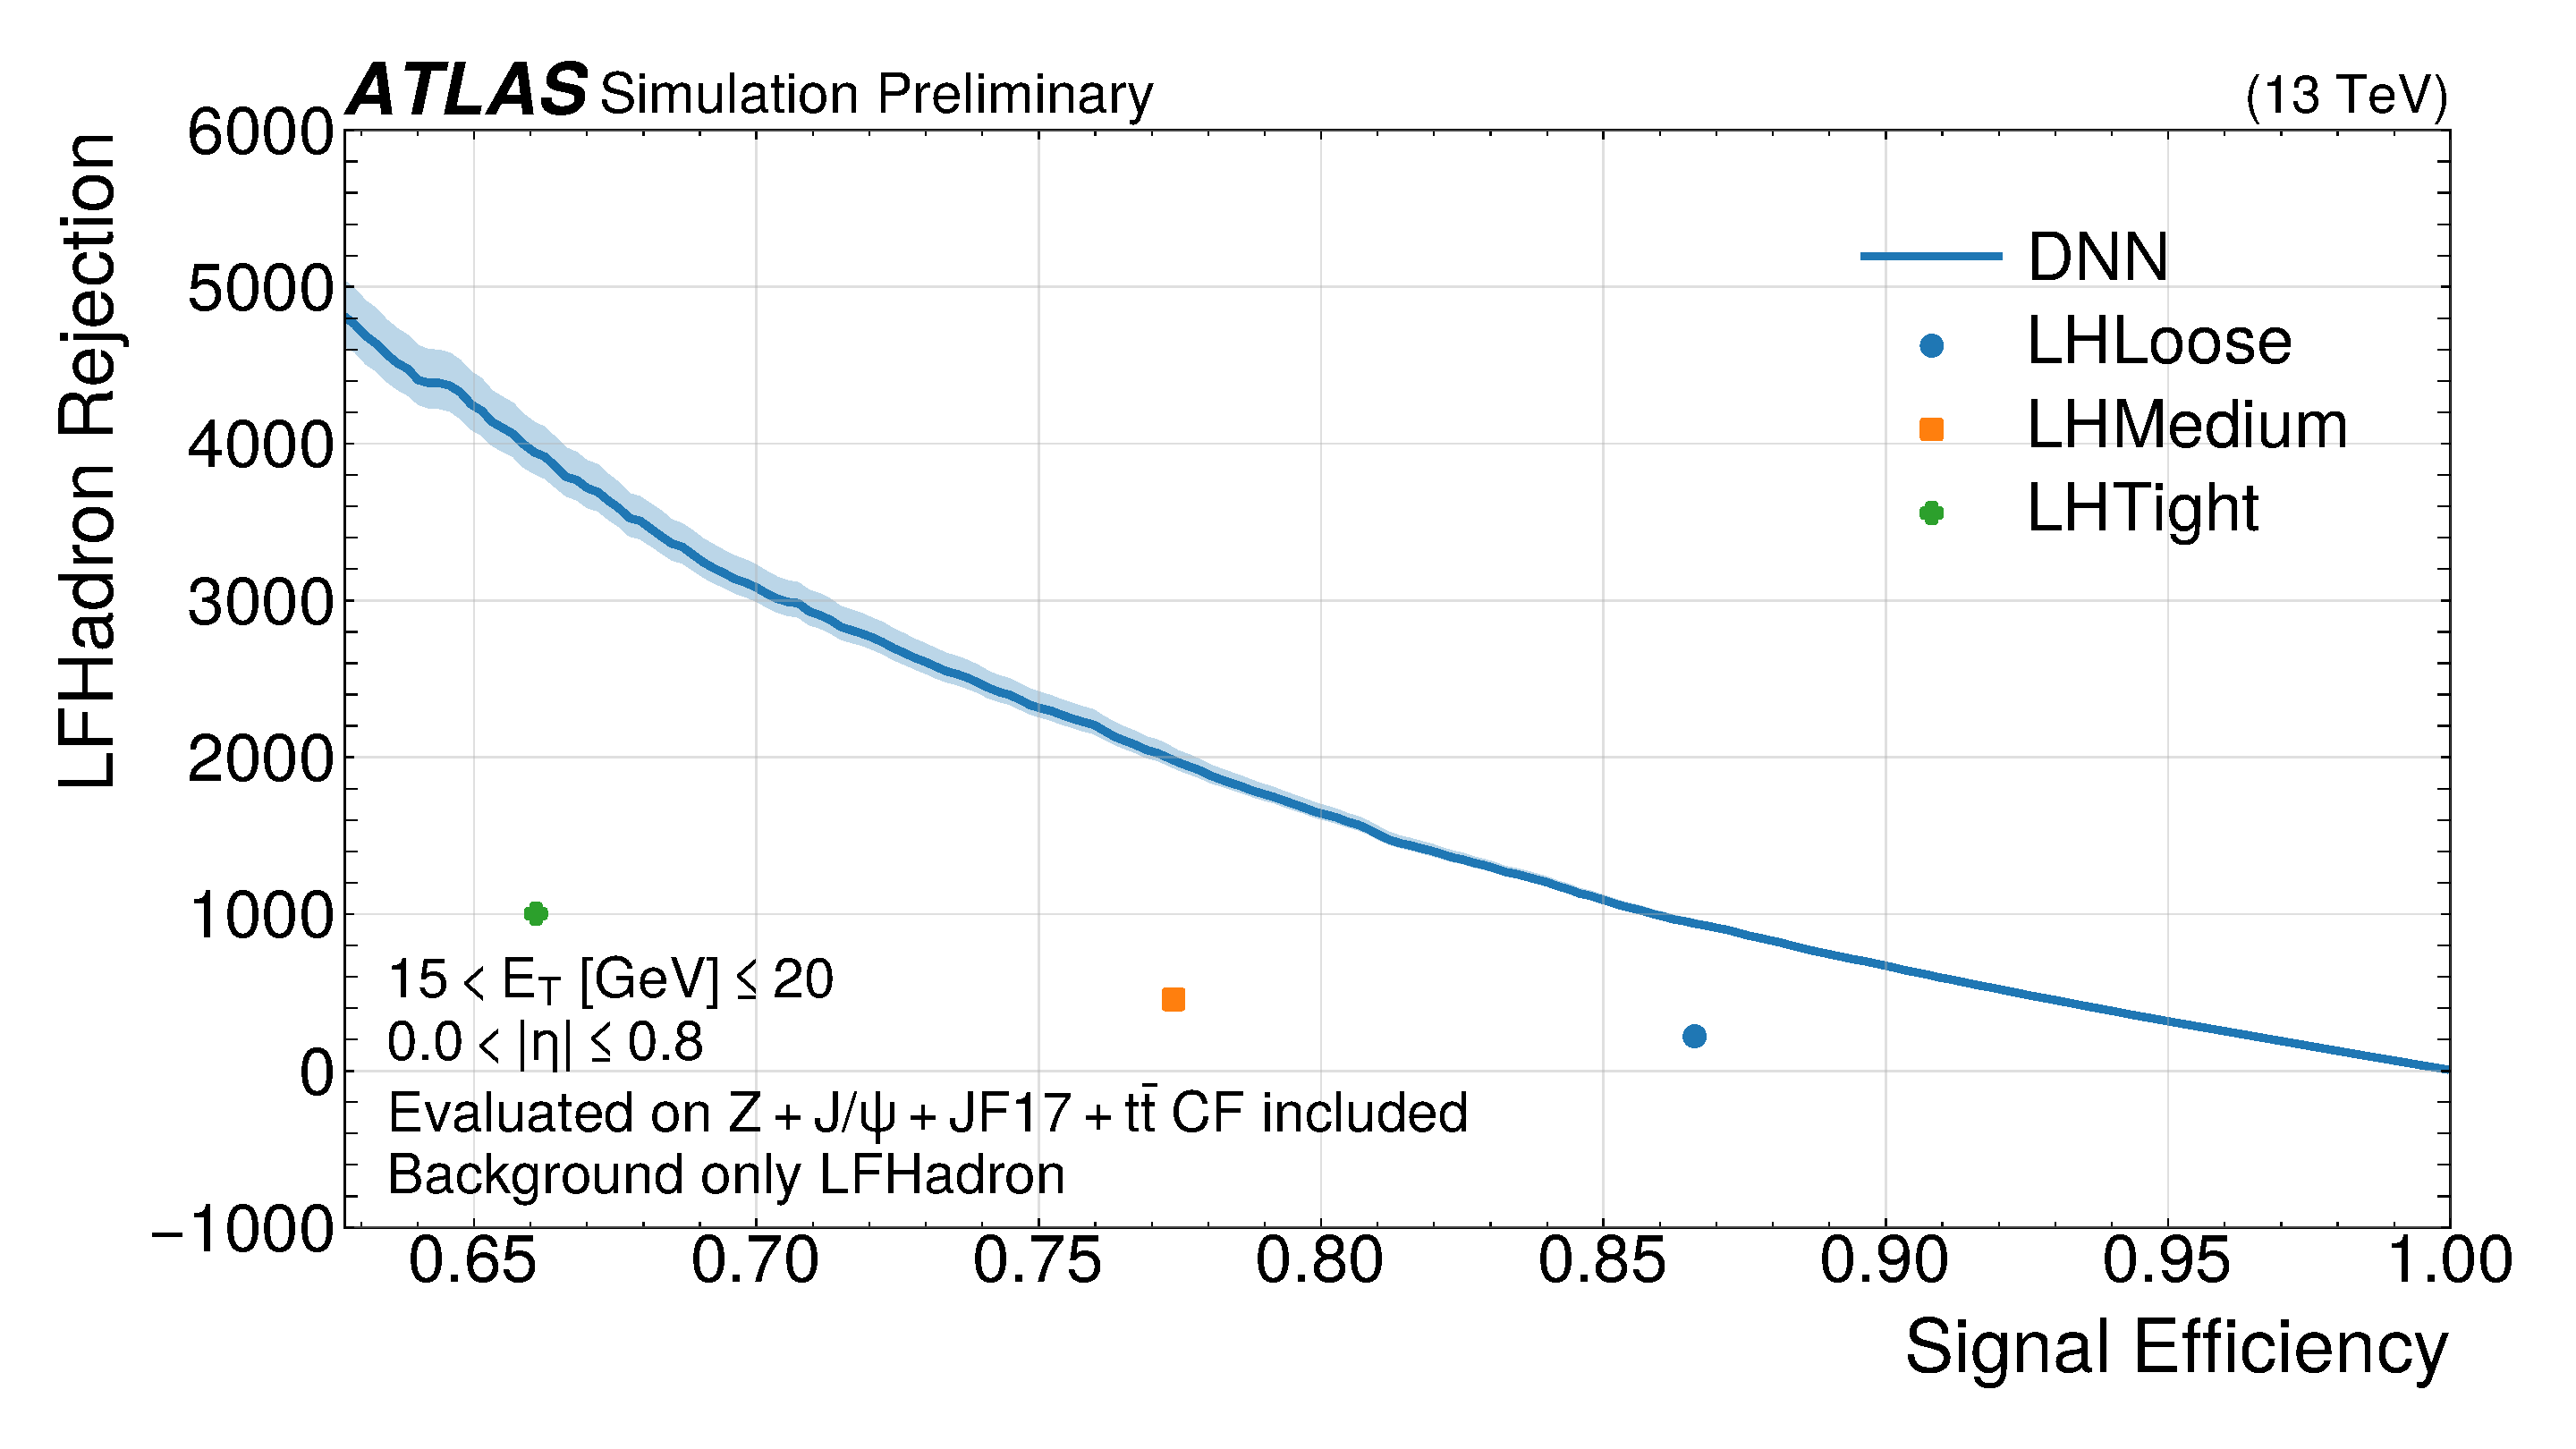
\includegraphics[width=\linewidth]{ROC/15_20_0p0_0p8/binnedROCCurveLFHadron_et15_20_eta0.0_0.8.pdf}
    \caption{}
    \label{fig:roc_lfh}
  \end{subfigure}

  \caption{Background rejection versus signal efficiency (ROC curves) for prompt electrons against:
  (a) all background classes combined,
  (b) electrons from Heavy-Flavour decays,
  (c) $e/\gamma$ from Light-Flavour decays,
  (d) Light-Flavour hadrons,
  and (e) photon conversions.
  Curves are shown for a representative $(E_{T}, |\eta|)$ bin, and the statistical uncertainties of the each background rejection are shown as bands.}
  \label{fig:roc_mainbkg}
\end{figure}


% --- Segunda figura ---
\begin{figure}[htbp]
  \centering
  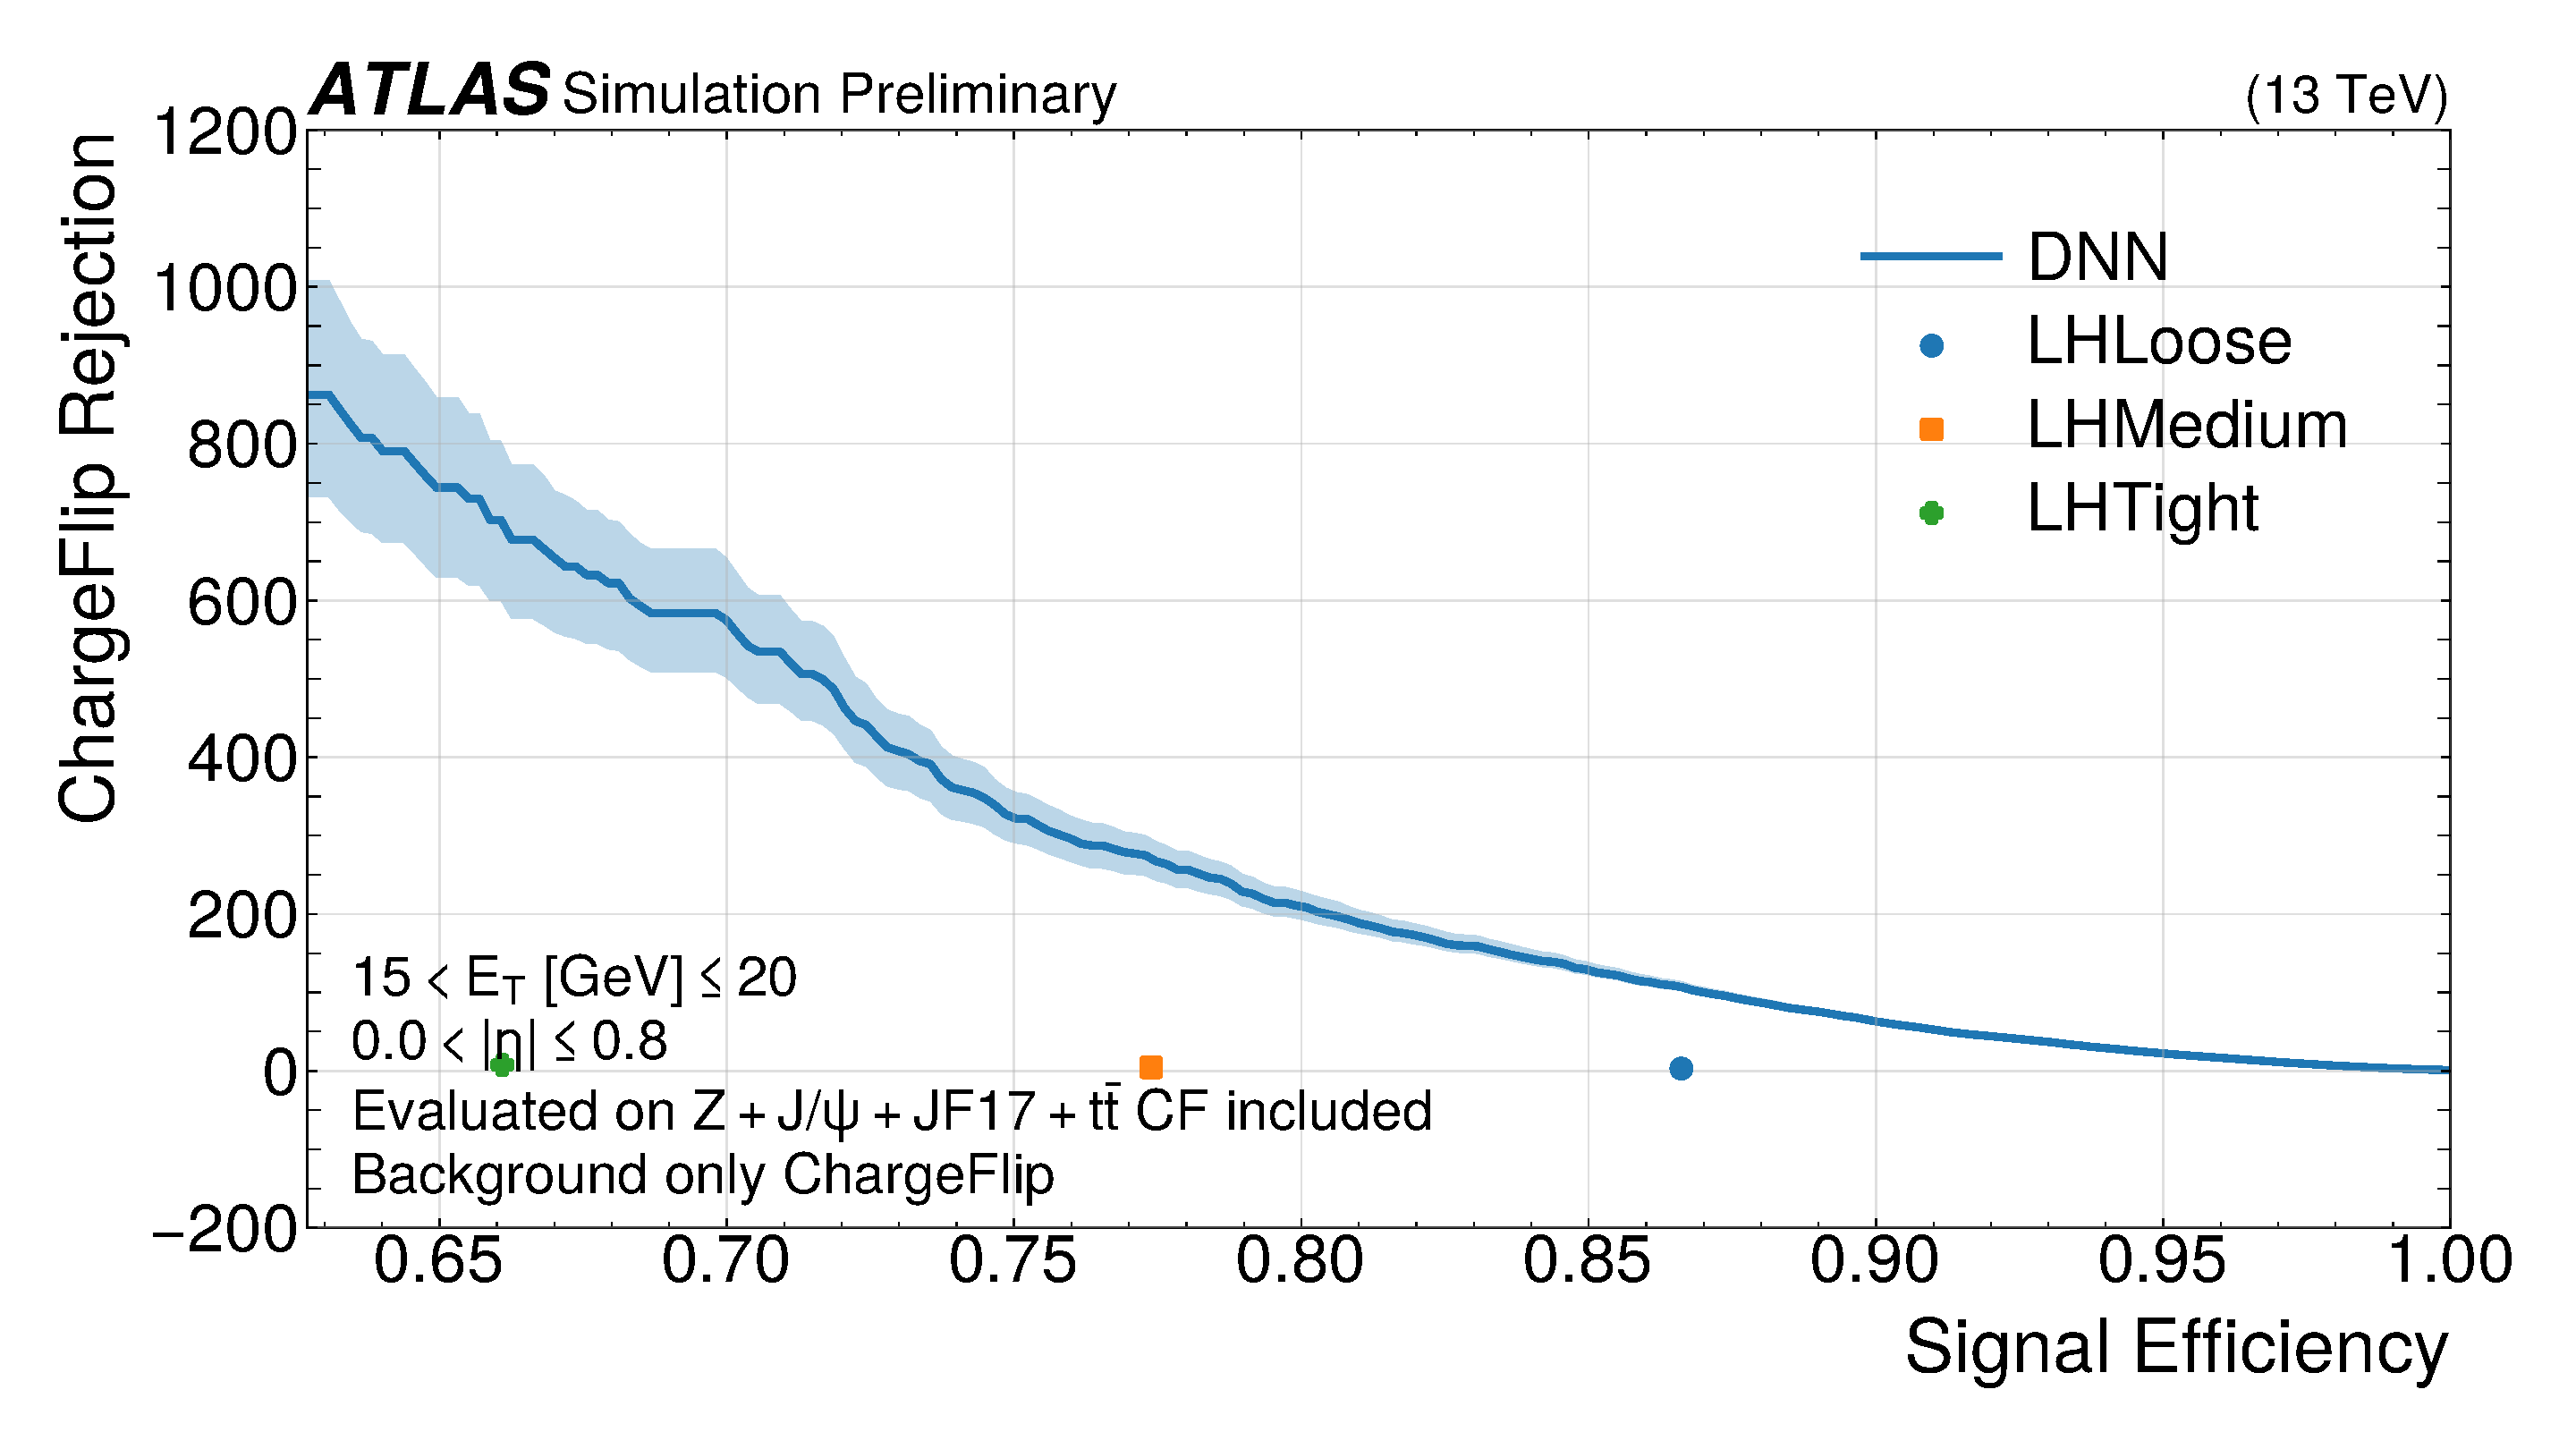
\includegraphics[width=0.6\linewidth]{ROC/15_20_0p0_0p8/binnedROCCurveChargeFlip_et15_20_eta0.0_0.8.pdf}
  \caption{Background rejection versus signal efficiency (ROC curve) for prompt electrons against Charge-Flip electrons in a representative $(E_{T}, |\eta|)$ bin, and the statistical uncertainties of the each background rejection are shown as bands}
  \label{fig:roc_cf}
\end{figure}

\subsubsection{Tuning and working points definition}
\label{dnn:tuning}

As a final step, we build the identification menu based on the DNN decision. This menu encapsulates the set of thresholds on the DNN discriminant previously studied, together with the additional rectangular cuts associated with each defined working point.

In our specific case, we combine two discriminants: $\mathcal{D}_{el}$, defined in Eq.~\ref{dnn_discriminant}, and $\mathcal{D}_{CF}$, defined as the simple ratio $\mathcal{D}_{CF} = p_{El}/p_{CF}$. The first discriminant is used, as already discussed, to separate both signal-electron classes from the main background sources for the most common physics analysis scenarios. For analyses sensitive to the electron charge in the final state, this can be complemented with the additional discriminant $\mathcal{D}_{CF}$, which exhibits strong separation power, as illustrated in Figure~\ref{fig:cf_discriminant}, even though the selected $|\eta|$ bin is not the most populated with these candidates. Charge-Flip electrons are more likely to appear at higher $|\eta|$, where they traverse a larger amount of detector material, increasing the probability of processes such as bremsstrahlung.

\begin{figure}[htbp]
  \centering
  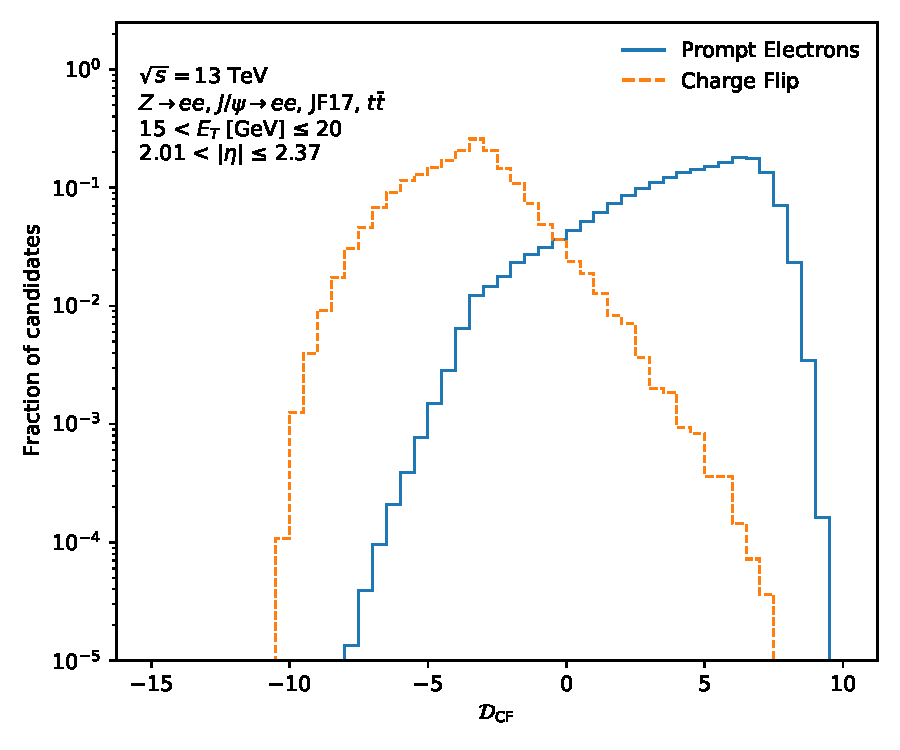
\includegraphics[width=0.6\linewidth]{discriminant_plots/panel_d.pdf}
  \caption{Charge-Flip discriminant $D_{\mathrm{CF}}$ of the DNN shown for prompt electrons and
  Charge-Flip electrons. Candidates satisfy $15<E_{T}\leq 20~\mathrm{GeV}$ and $0.0<|\eta|\leq 0.8$.}
  \label{fig:cf_discriminant}
\end{figure}

To obtain the identification menus, we first determine thresholds on the $\mathcal{D}_{el}$ discriminant, targeting specific signal identification efficiencies. These efficiencies are the same as those used to tune the LH discriminant, so we expect a similar signal identification performance. The procedure is carried out in the previously defined $\eta$ and $E_{\text{T}}$ bins, setting the discriminant threshold such that the fraction of signal electrons to the right of the cut matches the desired target efficiency.

Subsequently, for the resulting signal electron sample, the same procedure is applied to the $\mathcal{D}_{CF}$ discriminant. In this case, the target efficiencies correspond to those obtained with the Charge-Flip Electron Identifier (ECID)~\cite{Aaboud:2657964}, a complementary algorithm to LH used for this task. One of the advantages of the DNN is that it naturally incorporates both functionalities into a single output, and is potentially extendable to other definitions of electron candidates.

In addition, for the test electron dataset where these thresholds are defined, further requirements, parallel to those applied in LH, are imposed depending on the working point. These rectangular cuts are listed in Table~\ref{tab:wp_rectangular_cuts}.

\begin{table}[htbp]
  \centering
  \footnotesize
  \begin{tabular}{lcccc}
  \hline
  WP & $\texttt{BLayer}$ & $\texttt{Amb-bit}$ & $n_{\mathrm{pixel}}$ & $n_{\mathrm{Si}}$ \\
  \hline
  Loose  & 0 & $63$ & $\geq 1$ & $\geq 8$ \\
  Medium & $1$ & $63$ & $\geq 2$ & $\geq 8$ \\
  Tight  & $1$ & $35$ & $\geq 2$ & $\geq 8$ \\
  \hline
  \end{tabular}
  \caption{Additional selection on top of the discriminant for the different WPs, including requirements on the number of pixel and silicon hits.}
  \label{tab:wp_rectangular_cuts}
\end{table}
where the ambiguity bitmask is used to reject electron candidates with specific ambiguity types, ensuring that only candidates with reliable track-cluster associations are retained, and $\texttt{BLayer}$ essentially enforces the requirement of an additional hit in the insertable BLayer. In this way, the final menu is represented by two bidimensional matrices in terms of $\eta$ and $E_{\text{T}}$, together with the corresponding additional cuts.

%%%%%%%%%%%%%%%%%%%%%%%%%%%%%%%%%%%%%%%%%%%%%%%%%%%%%%%%%%%%%%%%%%%%%%%%%%%%%%%%%%%%%%%%%%%%%%%%%%%%%%%%%%%%%%%%%%%%%%%%%%%%%%%%%%%%%%%%%%%%%%%%%%%%%%%%%%%%%%%%%%%%%%%%%%%%%%%%%%%%%%%%%%%%%%%%%%%%%%%%%%%%
\section{Electron Isolation}
\label{electron_iso}

After the electron identification stage, it is common to apply additional isolation requirements in order to suppress objects other than signal electrons. In processes such as \zee, signal electrons are typically isolated, meaning that no significant activity is observed around them. In contrast, electrons originating from the decay of heavy-flavour hadrons, such as $b$-hadrons, may be accompanied by additional activity both in the calorimeter and in the tracking system. To reduce such contamination, isolation WPs are defined, based on thresholds applied to calorimeter and track isolation variables.

For track isolation, two main types of variables are used: $p_{\mathrm{T}}^{\mathrm{cone}XX}$ and $p_{\mathrm{T}}^{\mathrm{varcone}XX}$, where $XX$ can take values such as 20, 30, or 40. Both variables sum the total transverse momentum of all tracks surrounding the electron that are not associated with it. In the case of $p_{\mathrm{T}}^{\mathrm{cone}XX}$, all tracks within a fixed-radius cone of $\Delta R = 0.XX$ are considered. For $p_{\mathrm{T}}^{\mathrm{varcone}XX}$, the cone size is defined as $\Delta R = \min(10/p_{\mathrm{T}}, 0.XX)$. For example, $p_{\mathrm{T}}^{\mathrm{cone20}}$ sums the $p_{\mathrm{T}}$ of all tracks within a cone of $\Delta R = 0.2$. For isolation WPs, tracks must satisfy a vertex-association requirement and have $p_{\mathrm{T}}$ greater than 1~GeV or 0.5~GeV.

Similarly, calorimeter isolation is defined through the variable $E_{\mathrm{T}}^{\mathrm{topocone}XX}$, which corresponds to the sum of the transverse energy of topoclusters within a cone of radius $\Delta R = 0.XX$ around the electron. In this case, corrections are applied to account for energy leakage and pile-up effects.

\begin{table}[htbp]
\scriptsize
\centering
\label{tab:electron_isolation_vars}
\begin{tabular}{lccp{3cm}}
\hline
\textbf{Variable} & \textbf{Cone radius} & \textbf{Summed object} & \textbf{Description} \\
\hline
$p_{\mathrm{T}}^{\mathrm{cone}XX}$ & Fixed, $\Delta R = 0.XX$ & Tracks & Sums the $p_{\mathrm{T}}$ of all tracks not associated with the electron within a fixed-radius cone. \\
$p_{\mathrm{T}}^{\mathrm{varcone}XX}$ & Variable, $\Delta R = \min(10/p_{\mathrm{T}},\,0.XX)$ & Tracks & Same as $p_{\mathrm{T}}^{\mathrm{cone}XX}$ but with a cone size that decreases for high-$p_{\mathrm{T}}$ electrons. \\
$E_{\mathrm{T}}^{\mathrm{topocone}XX}$ & Fixed, $\Delta R = 0.XX$ & Topo-clusters & Sums the transverse energy of \textit{topo-clusters} within the cone. \\
\hline
\end{tabular}
\caption{Summary of the variables used in the definition of electron isolation in ATLAS. The cone radius, summed object, and whether the cone size is fixed or variable are indicated.}
\end{table}

%%%%%%%%%%%%%%%%%%%%%%%%%%%%%%%%%%%%%%%%%%%%%%%%%%%%%%%%%%%%%%%%%%%%%%%%%%%%%%%%%%%%%%%%%%%%%%%%%%%%%%%%%%%%%%%%%%%%%%%%%%%%%%%%%%%%%%%%%%%%%%%%%%%%%%%%%%%%%%%%%%%%%%%%%%%%%%%%%%%%%%%%%%%%%%%%%%%%%%%%%%%%
\section{Electron efficiency measurements}
\label{sec:electron_efficiency_measurements}
%General description of electron efficiency measurements, the whole chain, TagAndProbe, Ze+e- efficiency estimations (Ziso only mentioned, explain only Zmass), and also 2 words on Jpsi. 
%Mention that results must be combined.
%Maybe break it in 2 subsections.
%When we talk about Zmass, include a few figures about the the mass distributions and so on.

Ultimately, the true performance of any electron identification method must be evaluated on real data, especially in the context of specific physics analyses, where it is essential to determine with the highest possible precision the efficiency with which final-state electrons satisfy the chosen identification criteria.  

It is not only important to measure the identification efficiency in real data, but also to evaluate it on MC simulated samples, ensuring that simulated electrons are identified with an efficiency as close as possible to that observed in data. Since mismodellings and mismatches inevitably exist between simulation and real data, the determination of the so-called \emph{Scale Factors} (SFs) becomes crucial. SFs are simply defined as the ratio between the identification efficiency measured in data and that obtained in MC events. Their use is a very general practice in ATLAS, systematically applied not only for electron identification but also for other corrections such as lepton reconstruction and trigger efficiencies, jet energy scale and resolution, or $b$-tagging calibrations. In this way, SFs provide a consistent framework to align the performance of simulated samples with that observed in collision data.

In general, the total efficiency for selecting a true electron can be expressed as the product of the efficiencies associated with each selection step applied to the electron candidate:
\begin{equation}
  \epsilon_{\text{tot}} = \epsilon_{\text{reco}} \times \epsilon_{\text{ID}} \times \epsilon_{\text{iso}} \times \epsilon_{\text{trig}},
\end{equation}
where the first factor, $\epsilon_{\text{reco}}$, is computed independently of the others, as it quantifies the reconstruction efficiency, that is, the probability of correctly associating a reconstructed topological energy cluster to a true electron. The remaining efficiencies are measured with respect to the previous step. This is the case for the identification efficiency, which is the only one considered in this section for the DNN algorithm. It is defined as:
\begin{equation}
  \epsilon_{\text{ID}} = \frac{N^{\text{WP}}_{\text{ID}}}{N_{\text{reco}}},
\label{eq:id_eff}  
\end{equation}
where $N^{\text{WP}}_{\text{ID}}$ is the number of reconstructed electron candidates passing the identification working point under study, in our case defined using the DNN output, and $N_{\text{reco}}$ is the total number of electrons correctly reconstructed in the previous step.

Depending on the requirements imposed by the identification working point, the number of accepted electrons, and therefore the efficiency, will vary. Efficiencies are thus measured as a function of the different working points, and also in bins of $E_{\text{T}}$ and $\eta$, since the thresholds are parametrised in these variables. This approach provides a significant advantage: although, as will be shown in the following, efficiency measurements and SFs are derived using a specific physics process, their parametrisation makes them largely analysis-independent and suitable for use in any study involving electrons.

\subsection{Identification efficiency computation}
To determine the identification efficiency of the different WPs in data, an appropriate selection and treatment of the electron candidates is required in order to correctly handle the present backgrounds. The methods employed for this purpose are described in detail in Ref.~\cite{latest_electron_paper_2024}, while here they will be introduced briefly.

To obtain the purest possible dataset of signal electrons from collision data, it is essential to have the best possible control over the background. Since MC simulations are not fully accurate in modelling this contribution, we focus on the extraction of background templates from dedicated control regions, defined as regions of the phase space where specific selections enhance the background electron population. In our case, we concentrate on the measurement of SFs and signal identification efficiencies for electrons with $E_{\mathrm{T}} > 15$~GeV. Two methods are used to obtain a pure dataset of signal electrons and to model the background templates: the \zmass and \ziso methods.

Both approaches are based on events from the \zee resonance, initially selected through the Tag-and-Probe (\tp) technique, already introduced earlier, to obtain an unbiased set of electrons satisfying the ID WPs. In the \zmass method, background templates are obtained from the invariant mass distribution of the di-electron pair, while in the \ziso method they are derived from the distribution of a calorimeter isolation variable.

The \ziso method will not be further discussed here, as it is not used in this thesis. However, it is worth noting that the official ATLAS efficiency and SF results provided for other physics analyses are obtained by statistically combining both methods, leading to more robust results in terms of uncertainties. In the low-$E_{\mathrm{T}}$ region, below $15$~GeV, electron identification efficiencies are measured using $J/\psi \to e^+e^-$ decays, which provide a clean source of low-energy electrons. Backgrounds from non-prompt $J/\psi$ production, mainly originating from heavy-flavour hadron decays, are suppressed with invariant mass selections around the $J/\psi$ peak and isolation requirements, and their residual contribution is estimated using either template fits to the invariant mass and pseudo-proper lifetime distributions or cut-based methods that enhance the prompt fraction. Although not used in this thesis, the $J/\psi$ method is widely employed in ATLAS to extend the efficiency measurements to this low-$E_{\mathrm{T}}$ regime, and is then combined with the \zmass and \ziso results.

The binning used for these measurements is the same as that employed in the tuning of the DNN output, presented in Table~\ref{tune:binning}, excluding the low-energy region. The next section will describe in more detail how efficiencies are measured with the \zmass method and the selection applied.

\subsubsection{\zmass efficiency method}

The \zmass method for measuring identification efficiencies in data also requires Monte Carlo simulations. Unless otherwise stated, the results presented here use only Run-2 data from 2018, reprocessed with release R.22, together with a single simulated \zee\ sample as described in Sec.~\ref{subsec:electron_mc}. An identical baseline selection is applied to both collision data and simulations, and consistently used for both the LH and DNN identification menus.

Events are required to pass at least one of the single-electron triggers listed in Table~\ref{tab:electron_triggers_2018}. For the \tp\ pair, the tag electron must have transverse energy \et$>27$~GeV, lie within the ID acceptance $|\eta|<2.47$, and be outside the calorimeter crack region ($1.37<|\eta|<1.52$). Additional quality requirements are applied, including cuts on impact-parameter-related variables to suppress backgrounds and ensure the tag is a genuine electron. The tag must also satisfy the Tight WP of the corresponding algorithm (DNN or LH) and an isolation requirement $p_{\mathrm{T}}^{\mathrm{topocone20}}/p_{\mathrm{T}}<0.1$ to ensure track isolation. Finally, the tag is required to match the object that fired the trigger.

\begin{table}[htbp]
  \small 
  \centering
  \begin{tabular}{lc}
  \hline
  \textbf{Year} & \textbf{Electron triggers} \\
  \hline
  2018 & HLT\_e26\_lhtight\_nod0\_ivarloose \\
       & HLT\_e60\_lhmedium\_nod0 \\
       & HLT\_e140\_lhloose\_nod0 \\
       & HLT\_e300\_etcut \\
  \hline
  \end{tabular}
  \caption{Single-electron high-level triggers used in 2018 for this analysis.}
  \label{tab:electron_triggers_2018}
\end{table}

The probe electron is initially required to fulfil the same object-quality requirements, but no impact-parameter cuts are applied. A jet veto is imposed to ensure the electron candidate is isolated from any \antikt\ jet within a given cone. Minimum track-quality requirements are enforced ($n_{\mathrm{Si}} \ge 8$ and $n_{\mathrm{Pixel}} \ge 1$), together with \et$>15$~GeV. This \textit{preselected probe} is then tested against the identification working point (DNN or LH) under study.

For the \tp pair, both electrons must have opposite charge and an invariant mass within $75 < m_{e^+e^-} < 105$~GeV. If multiple valid pairs are found in an event (e.g.\ interchanging tag and probe), all are considered. Variations in the tag definition or in the invariant-mass window are treated as systematic uncertainties. Each variation is applied individually, and the efficiency difference with respect to the nominal choice is taken as the systematic variation. For example, the nominal isolation requirement $p_{\mathrm{T}}^{\mathrm{topocone20}}/p_{\mathrm{T}}<0.1$ is varied up and down to $<0.14$ and $<0.06$, respectively.

Recalling the definition of the identification efficiency in Eq.~\ref{eq:id_eff}, the denominator is composed of the preselected probes, while the numerator is the subset passing the identification menu under consideration. In practice, even when both electrons from the $Z$-boson resonance pass the ID requirements, non-negligible background can be present near the mass peak. Therefore, the signal identification efficiency is computed as:
\begin{equation}
  \small 
  \epsilon^{WP}_{\mathrm{ID}} = \frac{N^{\mathrm{WP}}_{\mathrm{ID}} - N_{\mathrm{bkg,ID}}}{N_{\mathrm{reco}} - N_{\mathrm{bkg,preselected\ probes}}},
\label{eq:id_eff}  
\end{equation}
where the background contribution in the signal region is estimated and subtracted prior to the calculation. This is precisely where the \zmass method plays its role.

In this method, the invariant mass $m_{e^+e^-}$ in the decay $Z\rightarrow e^+e^-$ is used as a discriminant between signal and background. The nominal mass range $75 < m_{e^+e^-} < 105$~GeV defines the signal region, while broader intervals are used to model and normalise the background. The method relies on template fits to separate the signal contribution from backgrounds, with templates for signal derived from simulated $Z\rightarrow e^+e^-$ events and templates for background obtained from dedicated data control regions.

In earlier implementations, background estimation under the $Z$ peak was performed by normalising the background template in the $m_{e^+e^-}$ sidebands. This approach was limited by biases from asymmetries between the low- and high-mass sidebands and by its strong dependence on simulation. The improved procedure adopted here, schematically shown in Fig.~\ref{fig:zmass_algo}, reduces the dependence on MC and optimises the subtraction of signal contamination from the background template. The method proceeds iteratively through the following main steps, separately for each $(E_{\mathrm{T}},\eta)$ bin:

\begin{figure}[htbp]
  \centering
  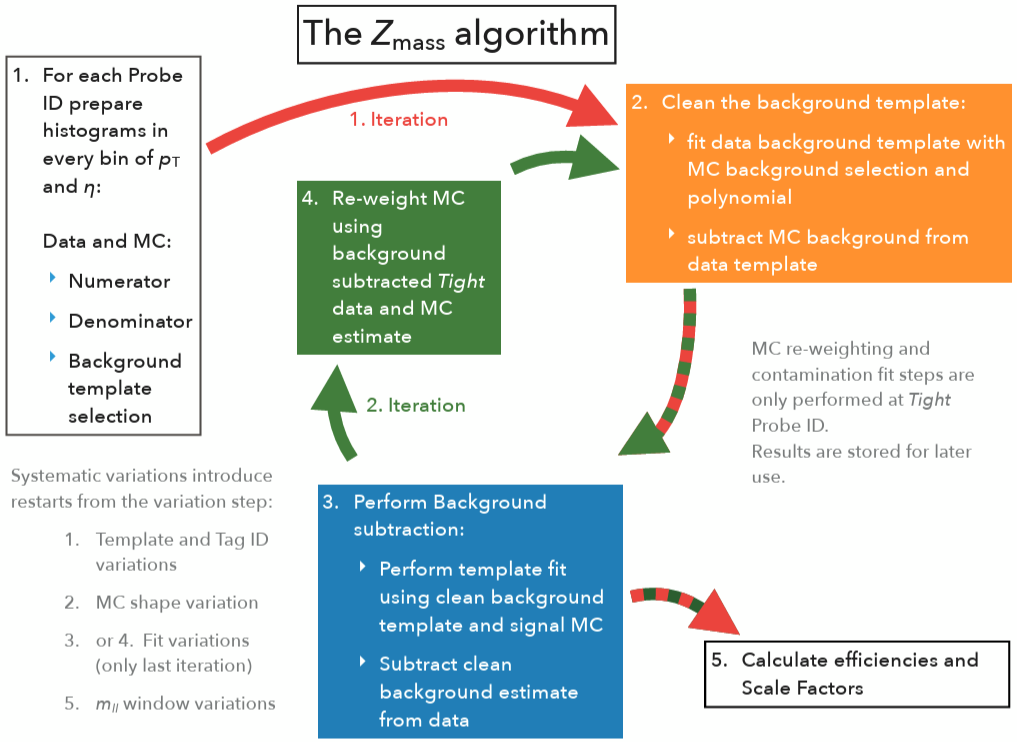
\includegraphics[width=0.8\linewidth]{zmass_diagram.png}
  \caption{Schematic view of the \zmass method for electron identification efficiency calculation. The five steps in which it consists are represented, where after the reweighting step, the second, third and fifth steps are repeated iteratively. Taken from Ref.~\cite{elias_thesis}. }
  \label{fig:zmass_algo}
\end{figure}

\begin{figure}[htbp]
  \centering
  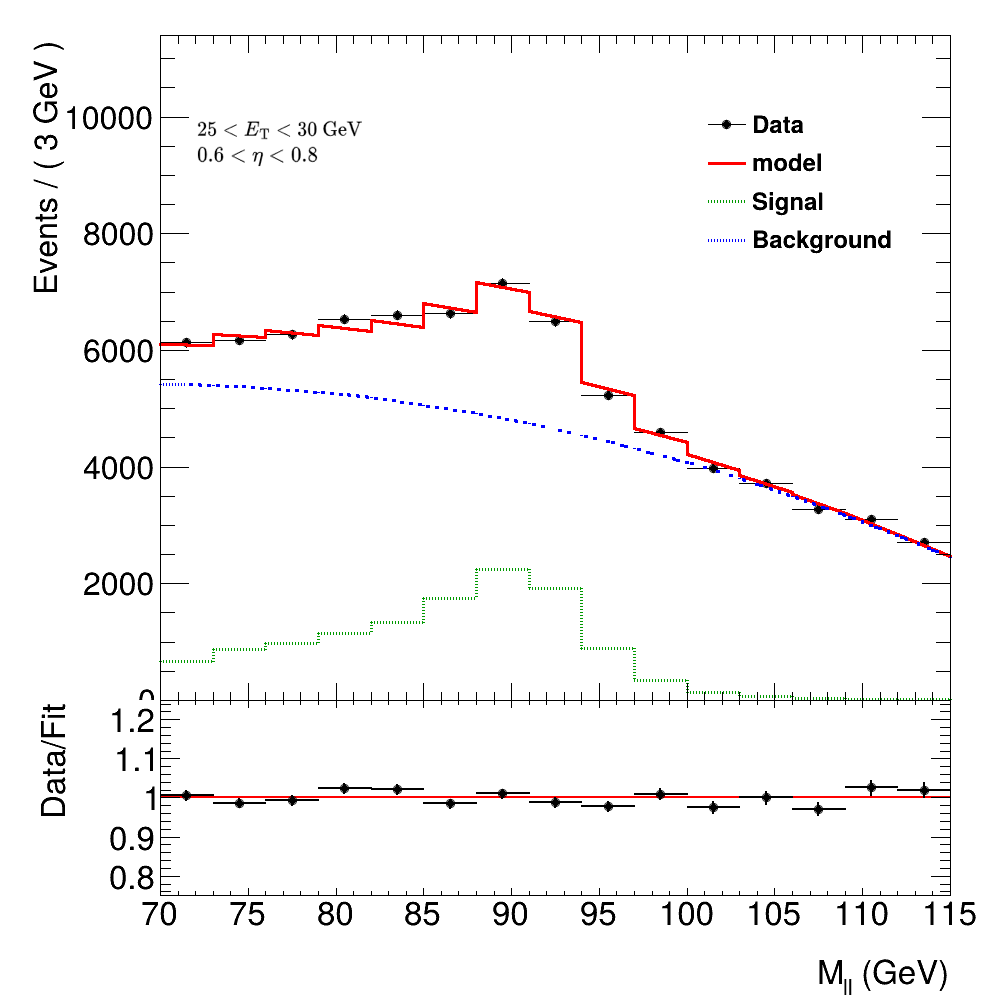
\includegraphics[width=0.6\linewidth]{plot_bkg_template_cleaning.png}
  \caption{Background cleaning procedure in the \zmass method for a representative $(E_{\mathrm{T}},\,|\eta|)$ bin. The data in the background-enriched control region is fitted with a polynomial function (red curve) describing the background component, together with a MC signal template representing the residual signal contamination. The cleaned background template, obtained after subtracting the signal contribution, is shown in blue.}
  \label{fig:bkg_clean}
\end{figure}

\begin{enumerate}
    \item \textbf{Background control region definition:} a background-enriched sample is selected by requiring the probe to fail a relaxed version of the Loose ID WP (either LH or DNN) and to satisfy a mild calorimeter isolation cut ($E_{\mathrm{T}}^{\mathrm{cone30}}/E_{\mathrm{T}}>0.12$). Signal templates are built from MC events fulfilling either numerator or denominator requirements, while background templates are taken from this control region in data, with MC providing the estimate of residual signal contamination.

    \item \textbf{Background template cleaning:} the residual signal present in the background control region is modelled as a sum of a polynomial background and an MC signal template in the $70 < m_{e^+e^-} < 115$~GeV range. The fitted signal component is subtracted from the data-driven background template to yield a “clean” background shape. Figure~\ref{fig:bkg_clean} shows this fit to data, with the background represented as a polynomial plus the signal template derived from MC in the mentioned mass range, yielding in blue the cleaned background template when removing the green (signal) contribution.

    \item \textbf{Background subtraction in the signal region:} the cleaned background template is normalised to the data in the signal region, in combination with the MC signal template, to extract the background yield. This yield is then subtracted from the total number of events to obtain the signal counts.

    \item \textbf{MC re-weighting:} before computing the efficiency, a re-weighting procedure is applied to correct for differences in the $Z$-boson line shape between data and simulation, which may arise from effects such as additional bremsstrahlung in the detector material.

    \item \textbf{Efficiency and scale factor extraction:} the identification efficiency in data is computed as in Eq.~\ref{eq:id_eff}, replacing $N_{bkg}$ by the background yields from the fit. MC efficiencies are evaluated as the simple ratio of identified probes to all preselected probes. Scale factors are then obtained from the ratio of data to MC efficiencies for each $(E_{\mathrm{T}},\eta)$ bin.
\end{enumerate}

As already mentioned, each step of the method introduces potential systematic uncertainties, evaluated by varying key aspects of the procedure, such as the background control region definition, the $m_{e^+e^-}$ fit range, the polynomial order in the signal contamination fit, or the tag electron isolation requirement. 
This is the procedure applied to measure the identification efficiencies in collision data. For the MC efficiency, Eq.~\ref{eq:id_eff} reduces to the simple initial ratio, since no background subtraction is required and the measurement can be performed using signal-only events.

The plots in Figure~\ref{fig:zmass_fit_dnn_medium} show examples of the signal-plus-background template fits obtained with the \zmass method, in the invariant mass distribution of the di-electron pairs. The left panel corresponds to the reconstructed probes, which form the denominator in the efficiency calculation, while the right panel shows the fits for the numerator probes passing the Medium DNN identification working point. These results are extracted from the case of the DNN identification menu, where the two discriminants defined in the previous sections are combined to build the selection. In both cases, the orange line represents the MC signal template, the blue line the estimated background, and the red line the sum of both contributions. The background level is significantly reduced when moving from the inclusive probe selection to the numerator probes passing the Medium ID, illustrating the increased purity of the sample as the identification requirements become stricter. 
The lower panels display the Data-to-Expectation ratio, highlighting the good agreement between data and the fitted templates in the mass range considered for the efficiency extraction. A slight degradation of the agreement is observed at very high invariant masses due to the limited statistics in that region, and a small percent-level discrepancy is also visible for the denominator case around the $Z$-boson peak. The latter is precisely the type of effect that the calculation of scale factors aims to correct.

\begin{figure}[htbp]
  \centering
  \includegraphics[width=0.9\linewidth]{hist_dnn_CFID_medium_mass.png}
  \caption{
    Signal and background template fits to the invariant mass $m_{e^{+}e^{-}}$ of the di-electron pairs for the \zmass\ method, shown for the reconstructed probes (left), which constitute the denominator in the efficiency calculation, and for the numerator probes passing the Medium DNN identification (right). The orange line shows the MC signal template, the blue line the estimated background, and the red line the sum of both contributions. The lower panels display the Data-to-Expectation ratio.}
  \label{fig:zmass_fit_dnn_medium}
\end{figure}


There is also the case in which we aim to test the background rejection power of the DNN identification menu in collision data.  
For this purpose, we employ the same method as before, but the event selection in this case starts from those events that have fired one of the prescaled triggers listed in Table~\ref{tab:electron_triggers_prescaled_2018}.  
In this case, none of these trigger strings include associated identification requirements, unlike in the signal case, in order to avoid introducing a selection bias.

\begin{table}[htbp]
  \centering
  \scriptsize
  \begin{tabular}{ll}
    \toprule
    \textbf{Year} & \textbf{Electron triggers (prescaled, \textit{etcuts})} \\
    \midrule
    2018 &
    HLT\_e4\_etcut, HLT\_e5\_etcut, HLT\_e9\_etcut \\
    & HLT\_e10\_etcut\_L1EM7, HLT\_e14\_etcut, HLT\_e15\_etcut \\
    & HLT\_e15\_etcut\_L1EM7, HLT\_e17\_etcut, HLT\_e20\_etcut\_L1EM7 \\
    & HLT\_e20\_etcut\_L1EM15, HLT\_e25\_etcut\_L1EM15, HLT\_e30\_etcut\_L1EM15 \\
    & HLT\_e40\_etcut\_L1EM15, HLT\_e40\_etcut\_L1EM9, HLT\_e50\_etcut \\
    & HLT\_e60\_etcut, HLT\_e80\_etcut, HLT\_e100\_etcut \\
    & HLT\_e120\_etcut, HLT\_e140\_etcut, HLT\_e160\_etcut \\
    & HLT\_e180\_etcut, HLT\_e200\_etcut, HLT\_e250\_etcut \\
    & HLT\_e300\_etcut \\
    \bottomrule
  \end{tabular}
  \caption{Prescaled \textit{etcuts} single-electron triggers used for background-electron selection in 2018, including Level-1 seeds where applicable.}
  \label{tab:electron_triggers_prescaled_2018}
\end{table}

In this way, we obtain a set fully composed of background electrons, allowing the treatment to follow the same approach as for the MC signal efficiency measurements, without the need to derive templates or subtract signal contamination.  
Therefore, in this case, to further reduce potential signal contamination, no tag electron is required, so that the only remaining signal comes from $W \to e\nu$ decays, which is negligible compared to the large QCD background faking electrons.  
For the probes, we apply exactly the same requirements as in the previous case, varying only the identification WP.  
Since no tag electron is required and the invariant mass loses its purpose, the electron counting for estimating the efficiency (or, in this case, the rejection $1/\epsilon$) is performed directly in $(E_{\text{T}},\eta)$ bins.


\subsection{Identification efficiency measurements: DNN versus LH}
%ID only vs LH? ID+CF should I show anything? Must be the default one, but regarding comparisons...
%Here we show eff vs pt. , eff vs eta (MC20, DATA18 AS ALWAYS), eff vs mu? Effs vs pt and eta, inclusive and in 1 pT bin. Need to derive them, since I only did it for ID+CF as far as I remember.

%We also show bkg rejection in Data, and the plots of the estimated significance which are also a good figure of merit of the improvement of DNN over LH.
%Some other plots to be shown? H4L plots maybe could be stolen?


The results presented in this section summarise the measured identification efficiencies and scale factors (SFs) for the DNN identification menu, as well as comparisons with the LH-based algorithm. Unless otherwise stated, all efficiencies are evaluated for $E_{\mathrm{T}}>15$~GeV and are shown for the three working points defined for the DNN, both in data and MC simulation. It is also worth noting that all MC efficiency measurements include the previously discussed shower-shape corrections.

Figure~\ref{fig:eff_sfs_dnn_vs_lh} displays the inclusive signal identification efficiency in data and MC, together with the corresponding SFs, for the three DNN working points without applying the charge-flip discriminant. The same selection is repeated using the LH identification menu, enabling a direct performance comparison in the case of the Medium WP. This comparison is shown separately in selected $(E_{\mathrm{T}},\eta)$ bins in order to highlight differences in specific kinematic regions. 

As illustrated in Figure~\ref{fig:eff_inclusive_pt_dnn_id}, the efficiency is typically reduced in the central barrel region ($|\eta|\sim0$) and in the transition region between barrel and end-cap ($1.37 < |\eta| < 1.52$). A general decrease in efficiency is also observed towards the end-cap, at large $|\eta|$ values. When studied as a function of $E_{\mathrm{T}}$, the identification efficiency is lower at small transverse energies. This behaviour originates from a larger background contamination in this regime, where the estimation of efficiencies with the \zmass method becomes more challenging, unlike at higher energies.

Concerning the SFs, the values for the three DNN working points remain close to unity, as expected given the corrections applied to the MC samples. The largest deviations are found for the Tight WP, which is reasonable since the stricter thresholds applied on the discriminant amplify potential mismodellings with respect to data and therefore affect the efficiency calculation more strongly. In general, the SFs tend to be closer to unity in the barrel region. A small asymmetry is also observed as a function of $\eta$, affecting all three WPs. Since the same feature is present in the LH measurements shown in Figures~\ref{fig:eff_dnn_lh_25_30},\ref{fig:eff_dnn_lh_0p1_0p6}, it cannot be attributed to the DNN algorithm itself.
\begin{figure}[htbp]
  \centering

  % Dos subfiguras arriba
  \begin{subfigure}{0.48\textwidth}
    \centering
    \includegraphics[width=\linewidth]{electron_eff_plots/DNN_ID_effs/DNNID_eff_vs_primary_cluster_be2_eta_for_pt_15p0_250p0.pdf}
    \caption{DNN signal identification efficiencies vs. $\eta$.}
    \label{fig:eff_inclusive_pt_dnn_id}
  \end{subfigure}
  \hfill
  \begin{subfigure}{0.48\textwidth}
    \centering
    \includegraphics[width=\linewidth]{electron_eff_plots/DNN_ID_effs/DNNID_eff_vs_pt_for_primary_cluster_be2_eta_-2p47_2p47.pdf}
    \caption{DNN signal identification efficiencies vs. \et.}
    \label{fig:eff_inclusive_eta_dnn_id}
  \end{subfigure}

  \vspace{0.6cm}

  % Dos subfiguras debajo
  \begin{subfigure}{0.48\textwidth}
    \centering
    \includegraphics[width=\linewidth]{electron_eff_plots/DNN_ID_effs/DNNID_LH_eff_vs_primary_cluster_be2_eta_for_pt_25p0_30p0.png}
    \caption{Comparison between DNN and LH in a representative $E_{\mathrm{T}}$ bin.}
    \label{fig:eff_dnn_lh_25_30}
  \end{subfigure}
  \hfill
  \begin{subfigure}{0.48\textwidth}
    \centering
    \includegraphics[width=\linewidth]{electron_eff_plots/DNN_ID_effs/DNNID_LH_eff_vs_pt_for_primary_cluster_be2_eta_0p1_0p6.png}
    \caption{Comparison between DNN and LH in a representative $\eta$ bin.}
    \label{fig:eff_dnn_lh_0p1_0p6}
  \end{subfigure}

  \caption{Signal identification efficiencies in data and MC, together with SFs, for the DNN menu without CF cuts. The top panel shows the inclusive efficiencies for the three working points, while the bottom panels illustrate the comparison with the LH algorithm in two representative $(E_{\mathrm{T}},\eta)$ bins.}
  \label{fig:eff_sfs_dnn_vs_lh}
\end{figure}

A direct comparison of the signal identification efficiency between both algorithms is shown in Figure~\ref{fig:eff_dnn_lh_25_30} as a function of $\eta$ for $25 < E_{\mathrm{T}} < 30$~GeV, and in Figure~\ref{fig:eff_dnn_lh_0p1_0p6} as a function of $E_{\mathrm{T}}$ for $0.1 < \eta < 0.6$. In both cases, the obtained values are very similar, which is expected since both menus were tuned to match the same target identification efficiencies, as described in Section~\ref{dnn:tuning}.

In addition, Figure~\ref{fig:eff_sfs_dnn_vs_lh_mu} presents the efficiency as a function of the average number of interactions per bunch crossing, $\mu$, for all three DNN working points, along with a direct comparison between DNN and LH for the Medium and Loose ones. For the three DNN working points, a decreasing trend is observed as pile-up increases, with the Tight WP being the most sensitive to these variations. Nevertheless, the comparison with LH in Figures~\ref{fig:eff_sfs_dnn_vs_lh_loose_mu,fig:eff_sfs_dnn_vs_lh_medium_mu} shows a similar trend, with the LH algorithm exhibiting slightly more stability. This behaviour can be explained by the fact that the LH menu applies explicit pile-up dependent corrections, whereas the DNN, by construction, has no direct notion of pile-up.

\begin{figure}[htbp]
  \centering
  % Inclusivo grande arriba
  \begin{subfigure}{0.70\textwidth}
    \centering
    \includegraphics[width=\linewidth]{electron_eff_plots/DNN_ID_mu_effs/DNNID_eff_vs_average_mu.pdf}
    \caption{Inclusive signal identification efficiency in data and MC, together with SFs, for the three DNN working points without CF cuts.}
    \label{fig:eff_sfs_dnn_mu}
  \end{subfigure}

  \vspace{0.6cm}

  % Dos subfiguras debajo
  \begin{subfigure}{0.48\textwidth}
    \centering
    \includegraphics[width=\linewidth]{electron_eff_plots/DNN_ID_mu_effs/loose_DNN_LH_eff_vs_average_mu.pdf}
    \caption{Comparison between DNN and LH in a representative $(E_{\mathrm{T}},\eta)$ bin.}
    \label{fig:eff_sfs_dnn_vs_lh_loose_mu}
  \end{subfigure}
  \hfill
  \begin{subfigure}{0.48\textwidth}
    \centering
    \includegraphics[width=\linewidth]{electron_eff_plots/DNN_ID_mu_effs/medium_DNN_LH_eff_vs_average_mu.pdf}
    \caption{Comparison between DNN and LH in another $(E_{\mathrm{T}},\eta)$ bin.}
    \label{fig:eff_sfs_dnn_vs_lh_medium_mu}
  \end{subfigure}

  \caption{Signal identification efficiency as a function of $\mu$ for the three DNN working points without CF cuts. A comparison between DNN and LH is also shown for the Medium working point.}
  \label{fig:eff_sfs_dnn_vs_lh_mu}
\end{figure}


%From here: background ==> DNN ID+CF VS. LH+ECIDS

It is not only necessary to draw conclusions from the performance on signal electrons, which are used for the tuning, but the background rejection power must also be investigated. Figure~\ref{fig:bkg_acceptance_mc} shows the background acceptance, simply defined as the number of background electrons passing each working point. This performance is compared between the combined DNN ID+CF menu and the LH+ECIDs, evaluated on the \texttt{JF17} MC background sample, which contains a mixture of QCD jet flavours as described in Section~\ref{subsec:electron_mc}. 

The results are shown as a function of $\eta$ in two $E_{\mathrm{T}}$ bins, one at lower energies and one at higher energies, illustrating the performance across part of the kinematic range. A clear improvement of the DNN algorithm over the LH is observed across the full $\eta$ range, as it allows significantly fewer background electrons to pass. This is also evident in the lower pads where the ratio between both methods is displayed. At higher $E_{\mathrm{T}}$, the performance of LH is particularly degraded in the crack region, highlighting the challenges of electron identification in this part of the detector.

%First MC JF17 since it's the easiest way to evaluate
\begin{figure}[htbp]
  \centering
  \begin{subfigure}{0.48\textwidth}
    \centering
    \includegraphics[width=\linewidth]{electron_eff_plots/bkg_rejection/bkg_jf17_comparison_pt_bin_20-25.png}
    \caption{}
    \label{fig:bkg_acceptance_jf17_20_25}
  \end{subfigure}
  \hfill
  \begin{subfigure}{0.48\textwidth}
    \centering
    \includegraphics[width=\linewidth]{electron_eff_plots/bkg_rejection/bkg_jf17_comparison_pt_bin_40-45.png}
    \caption{}
    \label{fig:bkg_acceptance_jf17_40_45}
  \end{subfigure}
\caption{Comparison between DNN and LH in a representative $(E_{\mathrm{T}},\eta)$ bins.}
\label{fig:bkg_acceptance_mc}
\end{figure}

%Total Integral between 75 and 105 GeV DNN ID : 426369.0
%Total Integral between 75 and 105 GeV DNN CFID : 28872.0
%Total Integral between 75 and 105 GeV LH : 209467.0
%Total Integral between 75 and 105 GeV LH+ECIDS : 34372.0

However, final decisions on the background performance cannot be extracted by looking at a single MC sample alone. For this reason, it is necessary to also examine real collision data. A complementary validation is performed on same-sign $Z\to e^{+}e^{-}$ events in data, which are largely populated by CF electrons. Figure~\ref{fig:cf_bkg_data} shows the invariant mass distribution around the $Z$-boson peak, requiring a tag and a probe electron passing the Medium WP of the identification menus displayed in different coloured lines. The identification menu providing the best rejection of CF electrons is the one yielding the lowest curve. 

It can be observed that the DNN menu, when only applying ID cuts (black), allows more CF electrons to pass, which is expected since in the original $\mathcal{D}_{el}$ (defined in Eq.~\ref{dnn_discriminant}), this class is treated as signal. However, when comparing the LH menu with the dedicated ECIDS method, and the DNN combined with cuts on both $\mathcal{D}_{el}$ and $\mathcal{D}_{CF}$, not only is the same rejection recovered but it is surpassed, without the need to train a dedicated algorithm. This improvement is mainly due to the inclusion of new variables in the DNN training. A reduction of about $16\%$ in CF electrons is achieved within the $[75,105]$~GeV interval around the $Z$-boson mass.

\begin{figure}[htbp]
  \centering
  \includegraphics[width=0.7\textwidth]{electron_eff_plots/bkg_rejection/InvariantMassComparison_points_with_ratio.pdf}
  \caption{Inclusive background efficiency in same-sign $Z\to e^{+}e^{-}$ events for DNN, LH, DNN+CF, and LH+ECIDs. Lower curves indicate better charge-misidentification rejection.}
  \label{fig:cf_bkg_data}
\end{figure}

Finally, background rejection values can also be computed directly in collision data as described previously. However, these results are not shown here. Instead, since small variations are observed not only in the background rejection but also in the signal identification performance, we present in Figure~\ref{fig:significance_block} an estimation of the significance for the DNN (ID-only) and LH menus, computed in data as
\begin{equation}
\hat{\sigma} = S_{\mathrm{eff}} \times \sqrt{\mathrm{Bkg}_{\mathrm{rej}}},
\end{equation}
for each working point of the DNN and LH menus. This metric, derived from the combination of signal efficiency and background rejection, provides a direct figure of merit for the expected sensitivity improvement when moving from LH to the DNN approach.


\begin{figure}[htbp]
  \centering

  % --- Row 1: Inclusive vs eta and vs pT ---
  \begin{subfigure}{0.48\textwidth}
    \centering
    \includegraphics[width=\linewidth]{electron_eff_plots/significance_data/significance_vs_pt_etaInclusive_GOOD_ONE.pdf}
    \caption{\small{Inclusive significance vs $|\eta|$.}}
    \label{fig:significance_inclusive_eta}
  \end{subfigure}\hfill
  \begin{subfigure}{0.48\textwidth}
    \centering
    \includegraphics[width=\linewidth]{electron_eff_plots/significance_data/significance_vs_eta_ptInclusive_GOOD_ONE.pdf}
    \caption{\small{Inclusive significance vs $E_{\mathrm{T}}$.}}
    \label{fig:significance_inclusive_pt}
  \end{subfigure}

  \vspace{0.55cm}

  % --- Row 2: Fixed-bin projections ---
  \begin{subfigure}{0.48\textwidth}
    \centering
    \includegraphics[width=\linewidth]{electron_eff_plots/significance_data/significance_vs_pt_etaBin_0.60_0.80.pdf}
    \caption{\small{Significance vs $E_{\mathrm{T}}$, $|\eta|\in[1.37,1.52]$.}}
    \label{fig:significance_vs_pt_etaBin}
  \end{subfigure}\hfill
  \begin{subfigure}{0.48\textwidth}
    \centering
    \includegraphics[width=\linewidth]{electron_eff_plots/significance_data/significance_vs_eta_ptBin_25_30.pdf}
    \caption{\small{Significance vs $|\eta|$, $E_{\mathrm{T}}\in[25,35]$~GeV.}}
    \label{fig:significance_vs_eta_ptBin}
  \end{subfigure}

  \caption{Significance estimator $S_{\mathrm{eff}} \times \sqrt{\mathrm{Bkg}_{\mathrm{rej}}}$ computed in data for the DNN and LH identification menus. Top: inclusive measurements versus $|\eta|$ (a) and $E_{\mathrm{T}}$ (b) for the three working points. Bottom: projections in fixed kinematic regions, shown versus $E_{\mathrm{T}}$ at fixed $|\eta|$ (c) and versus $|\eta|$ at fixed $E_{\mathrm{T}}$ (d).}
  \label{fig:significance_block}
\end{figure}

From these plots, both for the inclusive case in the top row and for the selected $\eta$ and $E_{\mathrm{T}}$ bins, the overall improvement of the DNN menu over the LH approach is evident. 
As particularly observed in the background rejection performance, the LH algorithm exhibits a clear degradation in the crack region, which is not present for the DNN. In this case, specific treatments were applied during training, such as masking problematic variables in that region in order to avoid mis-modelling effects.  

In addition, from the bottom ratio plots it can be seen that the improvement follows an approximately consistent trend. For intermediate to lower $E_{\mathrm{T}}$ values, the DNN shows its best relative performance, reaching a peak around $E_{\mathrm{T}}=30$~GeV. Overall, these results indicate that the DNN menu provides a more robust performance particularly in regions with larger background contribution.

